\documentclass[russian]{lecture-notes}
\usepackage[final]{graphicx}
\usepackage{amsmath}
\usepackage{amssymb}
\usepackage[normalem]{ulem}
\usepackage{tikz}

\title{Комбинаторика и теория графов\\Лекционный материал}
\lecturer{Посов Илья Александрович}
\notesauthor{Штейнберг Эмиль}
\date{осенний семестр 2021/2022}

\newenvironment{centeredgraph}[3]
{
	\begin{center}
		\begin{tikzpicture}[every node/.style={#1}, every edge/.style={#2}, every path/.style={#3}]
	}
	%here is the simple graph centered on the page
	{
		\end{tikzpicture}
	\end{center}
}

\newenvironment{tabulargraph}[3]
{
	\begin{tabular}{c}
		\begin{tikzpicture}[every node/.style={#1}, every edge/.style={#2}, every path/.style={#3}]
	}
	%here is the simple graph, which can be followed by a tabular
	{
		\end{tikzpicture}
	\end{tabular}
	~~~
}

\begin{document}

	\maketitle
	\section{Бинарные отношения}
	\subsection{Определение}
	\begin{definition}
		Пусть $m$ и $n$ --- некие непустые множества, $R$ --- подмножество произведения множеств $n \times m$, то есть всего множества пар из элементов $R$. \textit{Бинарным отношением} называется это множество $R$.
		\begin{example}
			Если $n = \{a,b,c\}$, то $n \times n = \begin{Bmatrix}aa & ba & ca\\ba & bb & bc\\ca & cb & cc\end{Bmatrix}$.
			Если $m = \mathbb{N}$, то $m \times m$ --- бесконечное множество из пар натуральных чисел.
		\end{example}
	\end{definition}
	
	\subsection{Обозначение}
	Бинарное отношение между двумя элементами $x$ и $y$ обозначается $(x,y) \in R$, однако мы будем использовать более привычное обозначение: $x R y$.
	
	\subsection{Примеры бинарных отношений}
	\begin{enumerate}
		\item Пусть $m = \mathbb{R}$. Возьмем такие $x$ и $y$, что $x > y$. Тогда:
		\begin{center}
			$3 R 2$, \sout{$3 R 4$} --- отношение \char34больше\char34.
		\end{center}
		\item Пусть $m = \mathbb{R}$. Возьмем такие $x$ и $y$, что $x \geq y$. Тогда:
		\begin{center}
			$7 R 6$, $7 R 7$, \sout{$7 R 8$} --- отношение \char34больше или равно\char34.
		\end{center}
		\item Пусть $m = \mathbb{R}$. Возьмем такие $x$ и $y$, что $x = y$. Тогда:
		\begin{center}
			$7 R 7$, \sout{$7 R 8$} --- отношение \char34равно\char34.
		\end{center}
		\begin{note}
			Далее будем обозначать подмножество $R$ более привычно: как выполняемое соотношение, например вместо $3 R 2$ будет использоваться $3 > 2$.
		\end{note}
		\item Пусть $m = \mathbb{R}$. Зададим бинарное отношение \char34примерно равно\char34 ($\approx$) при условии $|x-y|<1$. То есть, $5.5 \approx 5$, $213.1 \approx 212.11$, \sout{$1 \approx 2$}.
		\item Пусть $m = \mathbb{R}$. Зададим бинарное отношение \char34\#\char34, которое будет означать, что $x^2 > y$. То есть, $2 \# 3$, $4 \# 15$, \sout{$3 \# 9$}.
		\item Пусть $m = \mathbb{R} \cup \{0\}$. Зададим бинарное отношение делимости ($\vdots$), что будет означать, что найдется такое $p$, что $x = py$. То есть, $4~\vdots~2$, $100~\vdots~25$, \sout{$11~\vdots~4$}.
		\item Пусть $m$ --- множество прямых на плоскости. Зададим бинарное отношение параллельности ($\parallel$), которое будет означать, что прямые $l_1$ и $l_2$ либо не пересекаются, либо совпадают. То есть $l_1 \parallel l_2$ --- прямые параллельны (не пересекаются или совпадают), \sout{$l_1 \parallel l_2$} --- прямые не параллельны (пересекаются).
		\item Пусть $m$ --- множество прямых на плоскости. Зададим бинарное отношение перпендикулярности ($\perp$), которое будет означать, что прямые $l_1$ и $l_2$ пересекаются под прямым углом ($90^{\circ}$). То есть $l_1 \perp l_2$ --- прямые перпендикулярны (пересекаются под прямым углом), \sout{$l_1 \perp l_2$} --- прямые не перпендикулярны (пересекаются не под прямым углом).
		\item Пусть $m$ --- студент в ЛЭТИ. Зададим бинарное отношение \char34$\triangleright$\char34, которое будет означать, что средний балл студента $x$ больше, чем студента $y$. То есть, $x \triangleright y$ --- средний балл больше, \sout{$x \triangle y$} --- средний балл меньше или равен.
		\item Пусть $m$ --- пользователь Одноклассников. Зададим бинарное отношение \char34$\heartsuit$\char34, которое будет означать, что пользователь $x$ находится в друзьях у пользователя $y$. То есть, $x \heartsuit y$ --- пользователи в друзьях, \sout{$x \heartsuit y$} --- пользователи не в друзьях.
	\end{enumerate}
	Бинарные отношения можно задавать на любом множестве, главное, чтобы сопоставляемые элементы были элементами из одного множества.
	
	\subsection{Свойства}
	\begin{enumerate}
		\item \textbf{Определение.} Бинарное отношение $R$ называют \textit{рефлексивным}, если $\forall x \in m$ выполняется условие $xRx$.
		\begin{remark}
			Если подобрать один контрпример, то отношение не является рефлексивным. Это является примером того, что обычно обратное доказать проще, чем доказать прямо.
		\end{remark}
		\begin{example}
			\char34$\geq$\char34 --- рефлексивно, \char34=\char34 --- рефлексивно, \char34>\char34 --- не рефлексивно.
		\end{example}
		\item \textbf{Определение.} Бинарное отношение $R$ называют \textit{антирефлексивным}, если $\forall x \in m$ выполняется условие \sout{$xRx$}.
		\begin{remark}
			Существуют отношения не рефлексивные и не антирефлексивные, однако одновременно рефлексивных и нерефлексивных не может существовать (доказательство очевидно).
		\end{remark}
		\begin{example}
			\char34>\char34 и \char34<\char34 --- антирефлексивны, \char34\#\char34 (из примера 5) --- не рефлексивно и не антирефлексивно.
		\end{example}
		\item \textbf{Определение.} Бинарное отношение $R$ называют \textit{симметричным}, если $\forall x,y \in m$ выполняется условие $xRy = yRx$.
		\begin{example}
			\char34=\char34 --- симметрично, \char34>\char34 и \char34<\char34 --- не симметрично.
		\end{example}
		\item \textbf{Определение.} Бинарное отношение $R$ называют \textit{антисимметричным}, если $\forall x \neq y \in m$ выполняется условие $xRy =$~\sout{$yRx$}.
		\begin{example}
			\char34$\geq$\char34 и \char34$\leq$\char34 --- асимметричны.
		\end{example}
		\item \textbf{Определение.} Бинарное отношение $R$ называют \textit{асимметричным}, если $\forall x,y \in m$ выполняется условие $xRy =$~\sout{$yRx$}.
		\begin{example}
			\char34>\char34 и \char34<\char34 --- асимметричны.
		\end{example}
		\begin{proposition}
			Множество $R$ -- асимметрично означает то, что оно антисимметрично и и антирефлексивно.
		\end{proposition}
		\begin{remark}
			$\square$ (пустое отношение) --- асимметрично (не содержит ни одной пары на множестве $R$).
		\end{remark}
		\item \textbf{Определение.} Бинарное отношение $R$ называют \textit{транзитивным}, если $\forall x,y,z \in m$ при $xRy,~yRz$ выполняется условие $xRz$.
		\begin{example}
			\char34$>,~\geq$\char34 и \char34$<,~\leq$\char34 --- транзитивны, $\perp$ --- не транзитивно.
		\end{example}
	\end{enumerate}
	
	\begin{note}
		Свойства так же зависят от выбранного множества. Например, если взять делимость из примера 6, то оно является антисимметричным, однако для целых чисел ($x \in \mathbb{Z}$) отношение не будет являться антисимметричным ($4~\vdots~-4 = -4~\vdots~4$).
	\end{note}
	
	\subsection{Отношение эквивалентности}
	\begin{definition}
		Отношение $R$ называется \textit{отношением эквивалентности}, если $R$ --- рефлексивно, симметрично и транзитивно.
	\end{definition}
	\begin{example}
		Отношение равенства (\char34=\char34) является отношением эквивалентности на любом множестве.
		\begin{enumerate}
			\item $\forall x~x=x$ --- рефлексивно.
			\item $\forall x,y~x=y \Leftrightarrow y=x$ --- симметрично.
			\item $\forall x,y,z~x=y=z$ --- транзитивно.
		\end{enumerate}
		Также отношения $\parallel,~\equiv_n$ являются отношениями эквивалентности.\\
		Отношение \char34больше или равно\char34\ (\char34$\geq$\char34) не отношение эквивалентности.
	\end{example}
	
	Проверим следующее отношение:\\
	Отношение $\uparrow$ на множестве $\mathbb{N}$: выполняется условие $x \uparrow y$, если $x$ и $y$ содержат одинаковое количество цифр.
	\begin{example}
		$2 \uparrow 5,~12 \uparrow 42$, \sout{$3 \uparrow 33$}.
	\end{example}
	\begin{enumerate}
		\item $\forall x~x \uparrow x$ --- рефлексивно.
		\item $\forall x,y~x \uparrow y \Leftrightarrow y \uparrow x$ --- симметрично.
		\item $\forall x,y,z~x \uparrow y \uparrow z$ --- транзитивно.
	\end{enumerate}
	Отношение $\uparrow$ является отношением эквивалентности.
	
	\subsection{Классы}
	\begin{definition}
		Если $R$ является \textit{отношением эквивалентности} на множестве $\mathbb{M}$, и $x \in \mathbb{M}$, то $\mathbb{M}_x$ --- это набор таких $y$, что $xRy$.
	\end{definition}
	\begin{example}
		Равенство (\char34=\char34): $\mathbb{M}_5 = {5}$, $\equiv_3$: $\mathbb{M}_2 = \{2, 5, 8, \dots\}$, параллельность (\char34$\parallel$\char34): $\mathbb{M}_l$ содержит все прямые, параллельные $l$.
	\end{example}
	\begin{proposition}
		Если $R$ --- отношение эквивалентности на множестве $\mathbb{M}$, то при $\forall x,y \in \mathbb{M}$ $\mathbb{M}_x = \mathbb{M}_y$ или $\mathbb{M}_x \cap \mathbb{M}_y \neq \emptyset$.
	\end{proposition}
	\begin{proof}
		Если $\mathbb{M}_x \cap \mathbb{M}_y \neq \emptyset$, то существует $z \in \mathbb{M}_x$ и $\mathbb{M}_y$. Тогда $xRz$ и $yRz$, а по свойству симметричности $zRy$ и по свойству транзитивности $xRy$.
		
		Теперь проверим, что класс $\mathbb{M}_x = \mathbb{M}_y$. Возьмем $u \in \mathbb{M}_x$, проверим, что $u \in \mathbb{M}_y$. Мы знаем, что из $u \in \mathbb{M}_x$ следует, что $xRu$, а также и $xRy$, тогда по симметричности $yRx$, а по транзитивности $yRu$, значит $u \in \mathbb{M}_y$, то есть множества одинаковые.
	\end{proof}
	\begin{corollary}
		Если $R$ --- отношение эквивалентности на множестве $\mathbb{M}$, тогда $\mathbb{M}$ разбито на несколько классов эквивалентности, которые не пересекаются.
		$$\mathbb{M} = \mathbb{M}_1 \cup \mathbb{M}_2 \cup \dots \cup \mathbb{M}_n$$
	\end{corollary}
	\begin{example}
		Возьмем $\equiv_3$ на множестве $\mathbb{N}$. То есть:
		$$\mathbb{N} = \{0, 3, 6, \dots\} \cup \{1, 4, 7, \dots\} \cup \{2, 5, 8, \dots\}$$
	\end{example}
	\begin{remark}
		Если есть $\mathbb{M} \neq \emptyset$, разбитое на $\mathbb{M}_i \neq \emptyset$, тогда можно ввести отношения $R$.
		$$xRy,\text{ если для } \mathbb{M}_i~x,y \in \mathbb{M}_i$$
	\end{remark}
	\begin{example}
		Рассмотрим все прямые на плоскости --- это множество $\mathbb{M}$. Тогда среди всех прямых найдется бесконечное количество параллельных прямых. Здесь, отношение эквивалентности $R$ является параллельность (\char34$\perp$\char34), а классом $\mathbb{M}_i$--- их направление.
	\end{example}
	
	\subsection{Отношения порядка}
	Для простого понимания: имеется в виду не эквивалентность, а степени сравнения --- \textit{выше, лучше, сильнее, быстрее, важнее} и т.д.
	\begin{definition}
		Пусть дано бинарное отношение $R$, которое транзитивно, антисимметрично. Тогда, если оно:
		\begin{enumerate}
			\item Рефлексивно, то $R$ --- \textit{нестрогий порядок} ($\preceq/\succeq$).
			\item Антирефлексивно, то $R$ --- \textit{строгий порядок} ($\prec/\succ$).
		\end{enumerate}
	\end{definition}
	\begin{note}
		Введенные понятия:
		\begin{center}
			Если $a \succ b,~b \succ c$, то $a \succ c$ --- транзитивность.\\
			Если $a \succ b$, то \sout{$b \succ a$} --- антисимметричность.
		\end{center}
	\end{note}
	\begin{example}
		Отношение $>$ на $\mathbb{R}$ --- строгий порядок, $\geq$ на $\mathbb{R}$ --- нестрогий порядок,\linebreak$\vdots$ на $\mathbb{N}$ --- нестрогий порядок (число всегда делится само на себя).
	\end{example}
	\begin{definition}
		Пусть $R$ --- строгий или нестрогий порядок. Тогда $R$ называется \textit{линейным порядком}, если $\forall x \neq y$, то $xRy$ или $yRx$.
		\begin{remark}
			Если существуют такие $x$ и $y$, что \sout{$xRy$} или \sout{$yRx$}, то $R$ называют \textit{частичным порядком}.
		\end{remark}
	\end{definition}
	\begin{example}
		Рассмотрим некоторые примеры:
		\begin{enumerate}
			\item $>$ --- линейный порядок.
			\item $\geq$ -- линейный порядок.
			\item $\vdots$ --- частичный порядок.
		\end{enumerate}
	\end{example}
	\begin{proposition}
		Если $\succ$ --- строгий или нестрогий порядок на конечном множестве $\mathbb{M}$ $(\forall \alpha \in \mathbb{M}~|\alpha|<\infty)$. Тогда существует минимальный $x$, и для $\forall y \neq x$ \sout{$x \succ y$}.
	\end{proposition}
	\begin{example}
		Возьмем отношение $\geq$ на множестве $\{1, 2, 3, 4, 5\}$. Тогда минимальный $x = 1$, так как $\forall y$ \sout{$1 geq y$}.
	\end{example}
	\begin{proof}[Доказательство единственности]
		Берем $x_1$ --- любой элемент отношения $\succ$ конечного множества $\mathbb{M}$. Если он не минимальный, значит существует другой минимальный $x_2 \neq x_1$, такой что $x_1 \succ x_2$. Если же $x_2$ не минимальный, то существует другой минимальный $x_3 \neq x_2$, такой что $x_2 \succ x_3$. И так далее...
		
		Если мы не можем найти минимальный элемент, значит по свойству конечности множества $\mathbb{M}$ последний $x_i$ будет являться минимальным (точнее говоря, существующие $x_i$ будут повторяться).
		$$x_i \succ x_{i+1} \succ x_{i+2} \succ \cdots \succ x_{j-1} \succ x_j = x_i$$
		
		Отношение $\succ$ --- транзитивно, то есть $x_i \succ x_{j-1} \succ x_i$. А это невозможно по антисимметричности.
	\end{proof}

	\section{Топологическая сортировка}
	\begin{definition}
		Отношение $R_1$ на множестве $\mathbb{M}$ \textit{расширяет} $R_2$ на $\mathbb{M}$, если $R_2 \subset R_1$.
	\end{definition}
	\begin{remark}
		$R_1$ добавляет пары где $xRy$. То есть из $xR_2y$ следует, что $xR_1y$.
	\end{remark}
	
	\begin{theorem}[о топологической сортировке]
		Если отношение порядка $\succ$ --- строгое или нестрогое на конечном множестве $\mathbb{M}$, то существует $\gg$ --- отношение линейного порядка на $\mathbb{M}$, такое что $\gg$ расширяет $\succ$.
	\end{theorem}
	\begin{example}
		Пусть есть отношение порядка подчинения сотрудников:\\
		\begin{picture}(484,150)
		\put(80,120){\circle{22}}
		\put(72,116){ГД}
		\put(86,110){\vector(1,-3){6}}
		\put(98,81){\circle{22}}
		\put(90,77){О2}
		\put(74,110){\vector(-1,-3){6}}
		\put(62,81){\circle{22}}
		\put(54,77){О1}
		\put(68,70){\vector(1,-3){6}}
		\put(78,40){\circle{22}}
		\put(70,36){С2}
		\put(56,70){\vector(-1,-3){6}}
		\put(46,40){\circle{22}}
		\put(38,36){C1}
		\put(80,109){\vector(0,-1){57}}
		\qbezier(69,114)(32,100)(41,52)
		\put(39.2,60){\vector(1,-4){2}}
		\put(120,79){--- не линейный}
		\put(134,69){порядок}
		\multiput(292, 79)(65, 0){2}{или}
		\put(263,10){топологическая сортировка}
		\put(435,79){$\cdots$}
		\multiput(270,135)(0, -25){5}{\circle{16}}
		\multiput(270,127)(0, -25){4}{\vector(0,-1){9}}
		\multiput(335,135)(0, -25){5}{\circle{16}}
		\multiput(335,127)(0, -25){4}{\vector(0,-1){9}}
		\multiput(400,135)(0, -25){5}{\circle{16}}
		\multiput(400,127)(0, -25){4}{\vector(0,-1){9}}
		\fontsize{6pt}{1.2}
		\multiput(265,132)(65, 0){3}{$\text{ГД}$}
		\multiput(265,108)(65, 0){3}{$\text{О1}$}
		\put(265,83){$\text{О2}$}
		\multiput(330,83)(65, 0){2}{$\text{С1}$}
		\put(265,58){$\text{С1}$}
		\put(330,58){$\text{С2}$}
		\put(395,58){$\text{О2}$}
		\multiput(265,33)(65, 0){2}{$\text{О2}$}
		\put(395,33){$\text{С2}$}
		\end{picture}
		где ГД --- генеральный директор, О --- начальник отдела, С --- сотрудник.
	\end{example}
	
	\begin{proof}
		Найдем минимальный элемент отношения $\succ$ (пусть это $x_1 \in \mathbb{M}$) и удалим его из множества. Теперь имеем ограниченное отношение $\succ |_{\mathbb{M}-\{x_1\}}$. Очевидно, что это новое отношение имеет те же свойства, что и изначальное (антисимметрично, транзитивно и рефлексивно/антирефлексивно). В нем тоже есть минимальный элемент $x_2$, который мы удаляем и получаем ограниченное множество $\succ |_{\mathbb{M}-\{x_1, x_2\}}$. Продолжаем...
		
		В какой-то момент по свойству конечности множество $\mathbb{M}-\{\forall x_i\}$ станет пустым. Итого, имеем последовательность $\{x_1, x_2, \dots, x_n\}$, где $n = |M|$ --- размер исходного множества $\mathbb{M}$.
		
		Вводим новый порядок $x_i \ll x_j$ для $i < j$:
		$$x_1 \ll x_2 \ll \cdots \ll x_n$$
		
		\textbf{Почему $\ll$ расширяет $\prec$~?} 
		Если $x \prec y$, то $x$ был удален из множества раньше $y$, следовательно $x \ll y$.
	\end{proof}
	
	\begin{remark}
		Алгоритм поиска минимума и удаления не самый эффективный. Более эффективно будет сделать поиск в глубину и построить обратную нумерацию.
	\end{remark}
	
	\begin{remark}
		Топологическая сортировка --- практически важная задача. Как пример зависимостей: нельзя расдать листовки, пока они не напечатаны, при этом нельзя распечатать листовки, пока нет чернил и бумаги.
	\end{remark}
	
	\section{Транзитивное замыкание}
	По решению задачи топологической сортировки мы расширяли порядок до линейности. Теперь перед нами стоит задача расширить отношение до транзитивности.
	
	\begin{example}
		Пусть есть отношение подчиненности:\\
		\begin{center}
			\begin{picture}(150,100)
			\put(80,95){\circle{22}}
			\put(72,91){ГД}
			\put(86,85){\vector(1,-3){6}}
			\put(98,56){\circle{22}}
			\put(90,52){О2}
			\put(74,85){\vector(-1,-3){6}}
			\put(62,56){\circle{22}}
			\put(54,52){О2}
			\put(68,45){\vector(1,-3){6}}
			\put(78,15){\circle{22}}
			\put(70,11){С2}
			\put(56,45){\vector(-1,-3){6}}
			\put(46,15){\circle{22}}
			\put(38,11){С1}
			\color{red}
			\put(80,84){\vector(0,-1){57}}
			\qbezier(69,89)(32,75)(41,27)
			\put(39.2,35){\vector(1,-4){2}}
			\end{picture}
		\end{center}
		где ГД --- генеральный директор, О --- начальник отдела, С --- сотрудник.
		
		Черным цветом показана изначальная связь. Мы можем сказать, что $\text{ГД}R\text{О1}$ и $\text{О1}R\text{С1}$, но отсюда не следует, что $\text{ГД}R\text{С1}$.
		
		Для этого в множество необходимо добавить пару $\text{ГД}R\text{С1}$, чтобы отношение стало транзитивным (красный цвет). Аналогично для $\text{ГД}R\text{С2}$.
	\end{example}
	
	\begin{theorem}
		Пусть $R$ --- отношение на множестве $\mathbb{M}$ и существует такое отношение $\overline R$ на том же множестве, что:
		\begin{enumerate}
			\item $\overline R$ расширяет $R$ ($R \subset \overline R$).
			\item $\overline R$ --- транзитивно
			\item $\overline R$ --- минимальное транзитивное расширение, то есть если $\tilde R$ --- транзитивное расширение $R$, то $\tilde R \supset \overline R$.
		\end{enumerate}
	\end{theorem}
	
	\begin{proof}[Условное доказательство]
		Рассмотрим все транзитивные расширения отношения $\{\overline{R_i}\}$ и посчитаем $R$ как пересечение всех $\overline{R_i}$ (берем те ребра, которые есть только у транзитивного расширения).
		
		\begin{example}
			Пусть множество $\mathbb{M} = \{a,b,c,d\}$ и на нем есть отношения $aRb, bRc, bRd$. Мы можем его любым способом достроить до транзитивного (к примеру, достроим отношения $aRc,aRd,cRd$). Минимальным элементом $\overline R$ будет являться пересечение всех таких транзитивных отношений, и оно подходит под все условия:
			\begin{enumerate}
				\item $\overline R$ расширяет $R$ (пусть $xRy$, тогда $\forall \overline{R_i}~x \overline{R_i} y$, значит $x \overline R y$).
				\item $\overline R$ --- транзитивно (пусть $x \overline R y$, а $y \overline R z$, то $\forall \overline{R_i}~x \overline{R_i} y, y \overline{R_i} z$, значит $x \overline{R_i} z$, то есть $x \overline R z$).
				\item $\overline R$ --- минимальное транзитивное расширение (так как пересечение находится $\forall \overline{R_i}$).
				\item[0.] Существует ли $\overline{R_i}$?\\
				Скажем, что $R_1$ --- полное отношение = $\mathbb{M} \times \mathbb{M}$. Получили, что расширить можно в любом случае.
			\end{enumerate}
		\end{example}
	\end{proof}
	
	\section{Графы}
	\subsection{Неориентированный граф}
	\begin{definition}
		\textit{Неориентированный граф} $G$ --- это объект $(\mathbb{V}, \mathbb{E})$ от двух аргументов, где $\mathbb{V}$ --- множество \textit{вершин графа}, а $\mathbb{E} \subset \{(u,v),~u,v \in \mathbb{V}\}$ --- множество неупорядоченных пар из двух вершин (\textit{ребра графа}). Граф обладает хотя бы двумя вершинами, соединенными между собой.
	\end{definition}
	\begin{remark}
		Как рисовать:
		\begin{enumerate}
			\item Вершины обозначаются точками ($\cdot$) или кругами ($\circ$).
			\item Ребра обозначаются линиями между двумя вершинами. Важен только факт соединения.
		\end{enumerate}
	\end{remark}
	\begin{example}
		Граф (важно только наличие соединений, форма определяется фантазией):\\
		\begin{center}
			\begin{picture}(180, 100)
			\thicklines
			\put(10,90){\circle{32}}
			\put(90,60){\circle{32}}
			\put(30,20){\circle{32}}
			\put(25,84){\line(3,-1){50}}
			\put(43,30){\line(3,2){33}}
			\fontsize{48pt}{1.2}
			\put(130,48){$\text{=}$}
			\end{picture}
			\begin{picture}(100, 100)
			\thicklines
			\put(10,90){\circle{32}}
			\put(90,60){\circle{32}}
			\put(30,20){\circle{32}}
			\put(25,84){\qbezier(0,0)(45,30)(53,-13)}
			\put(43,30){\qbezier(0,0)(60,-15)(47,14)}
			\end{picture}
		\end{center}
	\end{example}
	\begin{definition}
		Граф $G$ называется \textit{полным}, если $\forall u,v \in \mathbb{V}~(u,v) \in \mathbb{E}$.
	\end{definition}
	\begin{note}
		$\mathbb{V}$ --- от слова \textit{vertex} (англ. вершина), $\mathbb{E}$ --- от слова \textit{edge} (англ. ребро).
	\end{note}
	
	\begin{definition}
		\textit{Размер} (порядок) графа определяется как количество вершин:
		$$|G| = |\mathbb{V}| = n$$
		Есои количество ребер $|\mathbb{E}| = m$, то иногда говорят, что $G$ --- это $(n,m)$-граф.
	\end{definition}
	
	\begin{definition}
		\textit{Степень вершины} $v \in \mathbb{V}$ --- это количество ребер, которым она принадлежит.
		$$\deg v = |\{(v,u)~|~(v,u) \in \mathbb{E}\}|$$
	\end{definition}
	
	\begin{definition}
		\textit{k-регулярным графом} называется граф, все степени вершин которого равны $k$.
	\end{definition}

	\subsection{Путь в графе}
	\begin{definition}
		\textit{Путь в графе} --- последовательность вершин-ребер
		$$v_1, e_1, v_2, e_2, \dots, v_n$$
		Причем, каждый $e$ ведет от вершины $v_i$ к $v_i+1$.
	\end{definition}
	
	\begin{example}
		$a,b,c,d$ --- подразумевается путь в графе от a к b, от b к c, и так далее.
	\end{example}
	
	\begin{definition}
		\textit{Замкнутый путь} --- такой путь, если первая и последняя вершина одинаковые.
	\end{definition}
	\begin{definition}
		\textit{Незамкнутый путь} --- такой путь, если первая и последняя вершина не совпадают.
	\end{definition}
	\begin{definition}
		\textit{Простой путь} --- такой путь, который содержит только различные ребра.
	\end{definition}
	
	\begin{example}
		Рассмотрим некоторые примеры путей:
		\begin{enumerate}
			\item $b,e,d,c,e$ --- простой путь, так как ребра не повторяются (однако вершина e повторяется).
			\item $a,b,c,d,e,c,d,e,b,a$ --- непростой замкнутый путь.
			\item Рассмотрим граф $G$:
			\begin{center}
				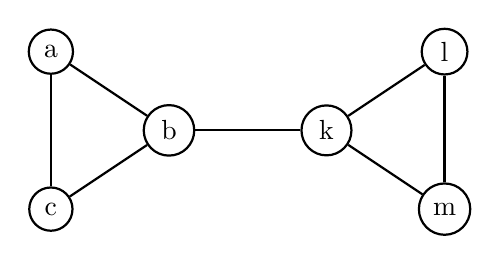
\begin{tikzpicture}[every node/.style={circle, draw=black, thick}, every path/.style={draw=black, thick}]
				\node (a) at (0,0) {a};
				\node (b) at (1.5,-1) {b};
				\node (c) at (0,-2) {c};
				\node (k) at (3.5,-1) {k};
				\node (l) at (5,0) {l};
				\node (m) at (5,-2) {m};
				
				\path (a) edge (b);
				\path (a) edge (c);
				\path (b) edge (c);
				\path (b) edge (k);
				\path (k) edge (l);
				\path (k) edge (m);
				\path (m) edge (l);
				\end{tikzpicture}
			\end{center}
			
			Путь $k,b,a,c,b,k$ --- не простой путь, так как ребро $e = (b,d)$ повторяется. А путь $b,c,a,b,k,l,m,k$ --- простой, так как ребра не повторяются.
		\end{enumerate}
	\end{example}
	
	\begin{definition}
		\textit{Циклом} называется замкнутый путь в графе, все вершины которого разные. \textit{Цепью} называется открытый путь в графе, все вершины которого разные (кроме первой с последней).
	\end{definition}
	
	\begin{example}
		Рассмотрим следующие графы:
		\begin{center}
			\begin{tikzpicture}[every node/.style={scale=0.4, circle, draw=black, thick}, every path/.style={draw=black, thick}]
			\node[scale=2.5] (a) at (0,0){};
			\node (b) at (1,1){};
			\node (c) at (2,0){};
			\node (d) at (1,-1){};
			\node[draw=white, scale=2.5] (text) at (3, 0) {--- цикл};
			
			\path (a) edge [bend left=40] (b);
			\path (b) edge [bend left=40] (c);
			\path (c) edge [bend left=40] (d);
			\path[->] (d) edge [bend left=40] (a);
			\end{tikzpicture}
			~~~~~
			\begin{tikzpicture}[every node/.style={scale=0.4, circle, draw=black, thick}, every path/.style={draw=black, thick}]
			\node[scale=2.5] (a) at (0,0){};
			\node (b) at (0.5,1){};
			\node (c) at (1,0){};
			\node (d) at (1.5,-1){};
			\node[scale=2.5] (e) at (2,0){};
			\node[draw=white, scale=2.5] (text) at (3, 0) {--- цепь};
			
			\path (a) edge [bend left=35] (b);
			\path (b) edge [bend left=35] (c);
			\path (c) edge [bend right=35] (d);
			\path[->] (d) edge [bend right=35] (e);
			\end{tikzpicture}
		\end{center}
		
	\end{example}
	
	\begin{theorem}
		Если между вершинами $u$ и $v$ существует путь, то существует и цепь между этими вершинами.
	\end{theorem}
	
	\begin{proof}
		Пусть есть путь $u, e_1, v_1, e_2, v_2, \dots, e_n, v$. Рассмотрим все такие возможные пути и возьмем самый короткий. Поймем, что это и есть \textit{цепь}. Представим, что какие то вершины совпали:
		$$u \dots v_i \dots v_j \dots v,~v_i = v_j$$
		Тогда среднюю часть можно убрать, и тогда это не самый короткий путь. Противоречие.
	\end{proof}
	
	\begin{theorem}
		Если есть простой замкнутый путь через ребро $e$, то есть и \textit{цикл} через это ребро.
	\end{theorem}
	
	\begin{proof}
		Аналогично предыдущей теореме, можно найти самый короткий путь, где ребро не повторяется.
	\end{proof}
	
	\subsection{Связность графа}
	\begin{definition}
		Граф $G$ --- \textit{связан}, если $\forall u,v \in \mathbb{V}$ существует цепь из $u$ в $v$.
	\end{definition}
	
	\begin{example}
		Рассмотрим следующие примеры:
		\begin{center}
			\begin{tikzpicture}[every node/.style={circle, draw=black, thick}, every path/.style={draw=black, thick}]
			\node (a) at (0,0){};
			\node (b) at (0,2){};
			\node (c) at (2,2){};
			\node (d) at (2,0){};
			\node (e) at (3.5,1){};
			\node[draw=white, rectangle] (text) at (1.75,-0.75) {связный};
			
			\path (a) edge (b);
			\path (b) edge (c);
			\path (c) edge (d);
			\path (d) edge (a);
			\path (c) edge (e);
			\path (d) edge (e);
			\end{tikzpicture}
			~~~~~~~~~~~~~~~~~~~~~~~~
			\begin{tikzpicture}[every node/.style={circle, draw=black, thick}, every path/.style={draw=black, thick}]
			\node (a) at (0,0){};
			\node (b) at (0,2){};
			\node (c) at (2,2){};
			\node (d) at (2,0){};
			\node (e) at (0.66,0.66){};
			\node (f) at (1.33,1.33){};
			\node[draw=white, rectangle] (text) at (1,-0.75) {не связный};
			
			\path (a) edge (b);
			\path (b) edge (c);
			\path (c) edge (d);
			\path (d) edge (a);
			\path (f) edge (e);
			\end{tikzpicture}
		\end{center}
	\end{example}
	
	Введем отношение $\equiv$ на вершинах графа: скажем, что $u \equiv v$, если существует путь из $u$ в $v$. Проверим, что $\equiv$ --- отношение эквивалентности:
	\begin{enumerate}
		\item Рефлексивно --- $u \equiv u$ (верно).
		\item Симметрично --- $u \equiv v$, следовательно $v \equiv u$ (верно).
		\item Транзитивно --- $u \equiv v$, $v \equiv w$, значит $u \equiv w$ (верно).
	\end{enumerate}
	
	\begin{definition}
		Классы эквивалентности $\equiv$ --- \textit{компоненты связности}.
	\end{definition}
	
	\begin{example}
		Пусть имеется граф:
		\begin{center}
			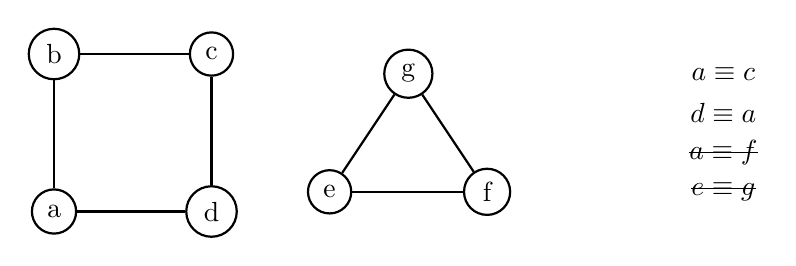
\begin{tikzpicture}[every node/.style={circle, draw=black, thick}, every path/.style={draw=black, thick}]
			\node (a) at (0,0){a};
			\node (b) at (0,2){b};
			\node (c) at (2,2){c};
			\node (d) at (2,0){d};
			\node (e) at (3.5,0.25){e};
			\node (f) at (5.5,0.25){f};
			\node (g) at (4.5,1.75){g};
			
			\node[draw=white, rectangle] (math1) at (8.5, 1.75) {$a \equiv c$};
			\node[draw=white, rectangle] (math2) at (8.5, 1.25) {$d \equiv a$};
			\node[draw=white, rectangle] (math3) at (8.5, 0.75) {\sout{$a \equiv f$}};
			\node[draw=white, rectangle] (math4) at (8.5, 0.25) {\sout{$e \equiv g$}};
			
			\path (a) edge (b);
			\path (b) edge (c);
			\path (c) edge (d);
			\path (d) edge (a);
			\path (e) edge (f);
			\path (f) edge (g);
			\path (g) edge (e);
			\end{tikzpicture}
		\end{center}
	\end{example}
	
	\begin{definition}
		$G^\prime$ --- называется \textit{подграфом G}, если из изначального графа выделить некоторые вершины, то есть он является подмножеством изначального множества вершин и ребер. По-научному, подграф $G^\prime$ определяется выражением:
		$$G^\prime = (\mathbb{V} \backslash \{v\}, \mathbb{E} \backslash \{(v,u)~|~(v,u) \in \mathbb{E}\})$$
	\end{definition}
	
	\begin{remark}
		$G$ является своим подграфом, а пустой граф $\emptyset$ --- подграфом любого графа.
	\end{remark}
	
	\begin{example}
		Граф $G^\prime$ является подграфом графа $G$:
		\begin{center}
			\begin{tikzpicture}[every node/.style={circle, draw=black, thick}, every path/.style={draw=black, thick}]
			\node (a1) at (0,0){a};
			\node (b1) at (0,2){b};
			\node (c1) at (1.5,1){c};
			\node (d) at (3.5,1){d};
			\node[draw=white, rectangle] (text1) at (1.75, 2.8) {Граф $G$:};
			
			\path (a1) edge (b1);
			\path (b1) edge (c1);
			\path (c1) edge (a1);
			\path (c1) edge (d);
			
			\node[draw=white, rectangle, scale=2.5] (symb) at (5,1) {$\supset$};
			
			\node (a2) at (6.5,0){a};
			\node (b2) at (6.5,2){b};
			\node (c2) at (8,1){c};
			\node[draw=white, rectangle] (text2) at (7.25, 2.8) {Граф $G^\prime$:};
			
			\path (a2) edge (b2);
			\path (b2) edge (c2);
			\path (c2) edge (a2);
			\end{tikzpicture}
		\end{center}
	\end{example}
	\begin{definition}
		Пусть существует граф $G$. Ребро $e$ называется \textit{мостом}, если при его удалении из графа количество компонентов связности $G$ < количество компонентов связности подграфов $G$.
	\end{definition}
	
	\begin{example}
		В графе $G$ ребра, выделенные красным, являются мостами:
		\begin{center}
			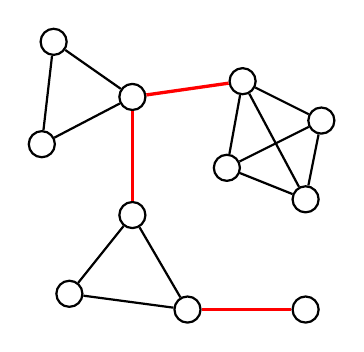
\begin{tikzpicture}[every node/.style={circle, draw=black, thick}, every path/.style={draw=black, thick}]
			\node (a) at (0,0){};
			\node (b) at (1.5,-0.2){};
			\node (c) at (0.8,1){};
			\node (d) at (3,-0.2){};
			\node (e) at (0.8,2.5){};
			\node (f) at (-0.35, 1.9){};
			\node (g) at (-0.2, 3.2){};
			\node (h) at (2.2,2.7){};
			\node (i) at (2,1.6){};
			\node (j) at (3.2,2.2){};
			\node (k) at (3,1.2){};
			
			\path (a) edge (b);
			\path (b) edge (c);
			\path (c) edge (a);
			\path (b) edge[very thick, draw = red] (d);
			\path (c) edge[very thick, draw = red] (e);
			\path (e) edge (f);
			\path (f) edge (g);
			\path (g) edge (e);
			\path (e) edge[very thick, draw = red] (h);
			\path (h) edge (i);
			\path (i) edge (j);
			\path (j) edge (h);
			\path (h) edge (k);
			\path (i) edge (k);
			\path (j) edge (k);
			\end{tikzpicture}
		\end{center}
	\end{example}
	
	\begin{definition}
		\textit{Степень связности графа G} --- это минимальное количество ребер, которое нужно удалить, чтобы граф $G$ стал несвязным. \textit{Двусвязный граф} --- граф степени связности не меньше двух, то есть \textbf{граф без мостов}.
	\end{definition}
	\begin{example}
		Некоторые примеры графов $n$-ной степени связности:
		\begin{center}
			\begin{tikzpicture}[every node/.style={circle, draw=black, thick}, every path/.style={draw=black, thick}]
			\node (a) at (0,0){};
			\node (b) at (2.5,0){};
			\node (c) at (2.5,2.5){};
			\node (d) at (0,2.5){};
			\node[draw=white, rectangle] (text) at (4.75,1.25){--- двусвязный граф};
			
			\path (a) edge (b);
			\path (b) edge (c);
			\path (c) edge (d);
			\path (d) edge (a);
			\end{tikzpicture}
			~~~~~
			\begin{tikzpicture}[every node/.style={circle, draw=black, thick}, every path/.style={draw=black, thick}]
			\node (a) at (0,0){};
			\node (b) at (2.5,0){};
			\node (c) at (2.5,2.5){};
			\node (d) at (0,2.5){};
			\node[draw=white, rectangle] (text1) at (4.75,1.25){--- граф 3-ей степени};
			\node[draw=white, rectangle] (text2) at (4.2,0.87){связности};
			
			\path (a) edge (b);
			\path (b) edge (c);
			\path (c) edge (d);
			\path (d) edge (a);
			\path (a) edge (c);
			\path (b) edge (d);
			\end{tikzpicture}
		\end{center}
	\end{example}
	
	\begin{definition}
		Вершина $v \in \mathbb{V}$ графа $G$ называется \textit{точкой сочленения}, если при ее удалении из графа (с ребрами) количество компонентов связности $G$ < количество компонентов связности подграфов $G$. В частном случае, точкой сочленения является вершина моста.
	\end{definition}
	
	Сосчитаем количество ребер в графе.
	\begin{theorem}
		В графе $G = (\mathbb{V}, \mathbb{E})$ количество ребер определяется как полусумма всех степеней вершин графа.
		$$|\mathbb{E}| = \frac{1}{2} \sum_{v \in \mathbb{V}} \deg v$$
	\end{theorem}
	\begin{proof}
		Мы знаем, что $\deg v$ --- количество ребер, выходящих из вершины. Складывая их, мы посчитали все ребра по два раза, так как у ребра ровно две вершины. Следовательно, чтобы получить количество ребер, нужно разделить это число на 2.
	\end{proof}
	\begin{corollary}
		Сумма степеней вершин графа $G$, а также количество его вершин с нечетной степенью всегда четные.
	\end{corollary}
	
	\begin{problem}
		На Землю прилетели 15 трехруких инопланетян. Могут ли они взяться за руки так, чтобы не было ни одной свободной руки?
	\end{problem}
	\textbf{Решение.} Нет, нельзя, так как количество вершин нечетной степени --- 15, а должно быть четное количество.
	
	\begin{definition}
		\textit{Висячая вершина} $v$ --- это вершина степени 1 ($\deg v = 1$).
	\end{definition}
	
	\begin{theorem}
		Если в графе $G$ нет висячих вершин, то существует \textit{цикл}.
	\end{theorem}
	
	\begin{proof}
		Берем ребро $e = (u_1, u_2)$ из конечного графа $G$. Мы знаем, что $u_2$ --- не висячая вершина, значит из нее есть какое-то другое ребро $e_1 = (u_2, u_3)$. $u_3$ --- тоже не висячая, и из нее тоже есть новое ребро. И так далее. Тогда по условию, в какой-то момент в графе вершина $u_n$ нового ребра $e_n$ точно совпадет с какой-то старой вершиной $u_i,~1 \leq i < n$. Получили цикл $u_i, u_{i+1}, \dots, u_n$.
	\end{proof}
	
	\begin{definition}
		\textit{Дерево} --- связный граф без циклов.
	\end{definition}
	
	\begin{example}
		Примеры деревьев:
		\begin{center}
			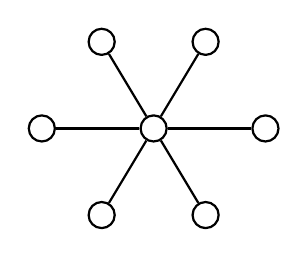
\begin{tikzpicture}[every node/.style={circle, draw=black, thick}, every path/.style={draw=black, thick}]
			\node (a) at (0,0){};
			\node (b) at (-1.42,0){};
			\node (c) at (1.42,0){};
			\node (d) at (0.66,1.1){};
			\node (e) at (-0.66,1.1){};
			\node (f) at (0.66,-1.1){};
			\node (g) at (-0.66,-1.1){};
			
			\path (a) edge (b);
			\path (a) edge (c);
			\path (a) edge (d);
			\path (a) edge (e);
			\path (a) edge (f);
			\path (a) edge (g);
			\end{tikzpicture}
			~~~~~~~~~~
			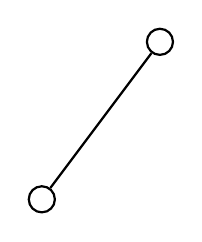
\begin{tikzpicture}[every node/.style={circle, draw=black, thick}, every path/.style={draw=black, thick}]
			\node (a) at (0,0){};
			\node (b) at (1.5,2){};
			
			\path (a) edge (b);
			\end{tikzpicture}
			~~~~~~~~~~
			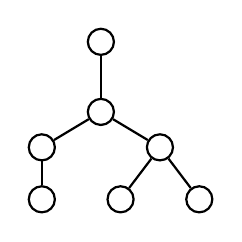
\begin{tikzpicture}[every node/.style={circle, draw=black, thick}, every path/.style={draw=black, thick}]
			\node (a) at (0,0){};
			\node (b) at (0,0.66){};
			\node (c) at (1,0){};
			\node (d) at (2,0){};
			\node (e) at (1.5,0.66){};
			\node (f) at (0.75,1.11){};
			\node (g) at (0.75,2){};
			
			\path (a) edge (b);
			\path (c) edge (e);
			\path (d) edge (e);
			\path (b) edge (f);
			\path (e) edge (f);
			\path (f) edge (g);
			\end{tikzpicture}
		\end{center}		
	\end{example}
	
	\begin{theorem}
		В любом дереве хотя бы две висячие вершины.
	\end{theorem}
	
	\begin{proof}
		Берем любую вершину. Если она не висячая, идем по ребру к следующей. Если снова не висячая, то продолжаем идти из нее. Так как циклы в графе отсутствуют, то в какой-то момент мы достигнем конца графа в висячей вершине. Теперь начнем путь из найденной вершины, и повторим алгоритм. Опять же, в какой-то момент мы упремся в висячую вершину. Итого, получили как минимум две висячие вершины.
	\end{proof}
	
	\begin{theorem}
		Если $G = (\mathbb{V}, \mathbb{E})$ --- дерево, то $|\mathbb{V}| = |\mathbb{E}| + 1$.
	\end{theorem}
	
	\begin{proof}[Доказательство по индукции]
		Пусть меняется количество вершин.
		\begin{enumerate}
			\item База: количество вершин $|\mathbb{V}| = 1$. Следовательно, $|\mathbb{E}| = 0$, то есть $|\mathbb{V}| = |\mathbb{E}| + 1$.
			\item Продолжение: рассмотрим произвольное дерево и найдем висячую вершину и удалим ее вместе с единственным ее ребром. При этом граф остался деревом, так как циклы не появились, и он остался связным, а $|\mathbb{E}|$ и $|\mathbb{V}|$ уменьшились на единицу. Продолжая, получим дерево из одной вершины, а по базе теорема сходится.
		\end{enumerate}
	\end{proof}

	\section{Полный граф}
	\begin{theorem}
		Если есть $n$ вершин, то:
		\begin{enumerate}
			\item $C^2_n = {n(n-1) \over 2}$ ребер.
			\item Степени всех вершин $n-1$. Так как $\sum_{v \in \mathbb{V}} \deg v = 2|E|$, то $|E| = {n(n-1) \over 2}$
		\end{enumerate}
	\end{theorem}
	
	\begin{example}
		Следующие графы являются полными:
		\begin{center}
			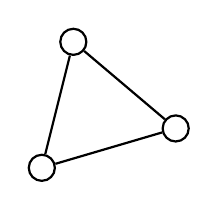
\begin{tikzpicture}[every node/.style={circle, draw=black, thick}, every path/.style={draw=black, thick}]
			\node (a) at (0,0){};
			\node (b) at (1.7,0.5){};
			\node (c) at (0.4,1.6){};
			
			\path (a) edge (b);
			\path (a) edge (c);
			\path (b) edge (c);
			\end{tikzpicture}
			~~~~~~~~~~
			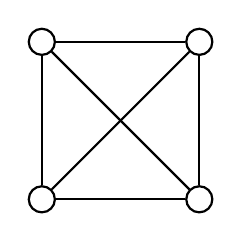
\begin{tikzpicture}[every node/.style={circle, draw=black, thick}, every path/.style={draw=black, thick}]
			\node (a) at (0,0){};
			\node (b) at (2,0){};
			\node (c) at (2,2){};
			\node (d) at (0,2){};
			
			\path (a) edge (b);
			\path (a) edge (c);
			\path (a) edge (d);
			\path (b) edge (c);
			\path (b) edge (d);
			\path (c) edge (d);
			\end{tikzpicture}
			~~~~~~~~~~
			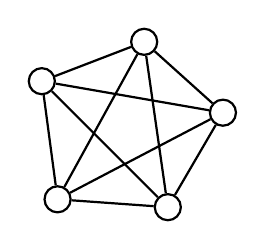
\begin{tikzpicture}[every node/.style={circle, draw=black, thick}, every path/.style={draw=black, thick}]
			\node (a) at (0,0){};
			\node (b) at (-0.2,1.5){};
			\node (c) at (1.1,2){};
			\node (d) at (2.1,1.1){};
			\node (e) at (1.4,-0.1){};
			
			\path (a) edge (b);
			\path (a) edge (c);
			\path (a) edge (d);
			\path (a) edge (e);
			\path (b) edge (c);
			\path (b) edge (d);
			\path (b) edge (e);
			\path (c) edge (d);
			\path (c) edge (e);
			\path (d) edge (e);
			\end{tikzpicture}
		\end{center}
	\end{example}
	
	\section{Планарные графы}
	\begin{definition}
		\textit{Планарные графы} --- это те графы, которые можно нарисовать на плоскости так, чтобы ребра не пересекались.
	\end{definition}
	
	\begin{example}
		Пример \char34правильного\char34~и \char34неправильного\char34~планарных графов:
		\begin{center}
			\begin{tikzpicture}[every node/.style={circle, draw=black, thick}, every path/.style={draw=black, thick}]
			\node[rectangle, draw=white] (text1) at (-2.375,1){правильный граф};
			
			\node (a1) at (0,0){};
			\node (b1) at (0,2){};
			\node (c1) at (2,2){};
			\node (d1) at (2,0){};
			
			\path (a1) edge (b1);
			\path (b1) edge (c1);
			\path (c1) edge (d1);
			\path (d1) edge (a1);
			
			\node[rectangle, draw=white, scale=2] (equal) at (3.25,1){$\simeq$};
			
			\node (a2) at (4.5,0){};
			\node (b2) at (6.5,2){};
			\node (c2) at (4.5,2){};
			\node (d2) at (6.5,0){};
			
			\path (a2) edge (b2);
			\path (b2) edge (c2);
			\path (c2) edge (d2);
			\path (d2) edge (a2);
			
			\node[rectangle, draw=white] (text1) at (9.125,1){неправильный граф};
			\end{tikzpicture}
		\end{center}
	\end{example}
	
	\begin{theorem}[\textbf{Формула Эйлера}]
		Если связный планарный граф $G = (\mathbb{V}, \mathbb{E})$ нарисован на плоскости, то у него можно посчитать \textit{грани} $f$. Пусть $|\mathbb{V}| = n, |\mathbb{E}| = m$. Тогда:
		$$n-m+f = 2$$
	\end{theorem}
	
	\begin{problem}
		Посчитать грани следующих графов:
		\begin{center}
			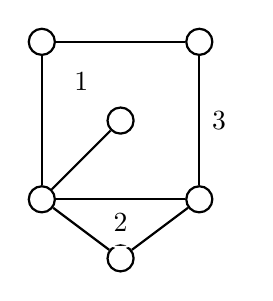
\begin{tikzpicture}[every node/.style={circle, draw=black, thick}, every path/.style={draw=black, thick}]
			\node (a) at (0,0){};
			\node (b) at (0,2){};
			\node (c) at (2,2){};
			\node (d) at (2,0){};
			\node (e) at (1,1){};
			\node (f) at (1,-0.75){};
			
			\node[draw=white] (f1) at (0.5,1.5){1};
			\node[draw=white] (f2) at (1,-0.3){2};
			\node[draw=white] (f3) at (2.25,1){3};
			
			\path (a) edge (b);
			\path (b) edge (c);
			\path (c) edge (d);
			\path (d) edge (a);
			\path (a) edge (e);
			\path (d) edge (f);
			\path (a) edge (f);
			\end{tikzpicture}
			~~~~~~~~~~
			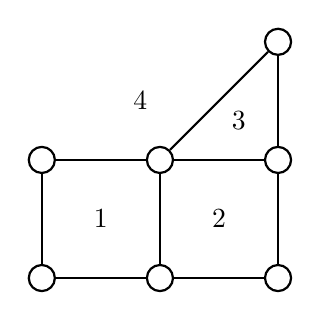
\begin{tikzpicture}[every node/.style={circle, draw=black, thick}, every path/.style={draw=black, thick}]
			\node (a) at (0,0){};
			\node (b) at (0,1.5){};
			\node (c) at (1.5,1.5){};
			\node (d) at (1.5,0){};
			\node (e) at (3,1.5){};
			\node (f) at (3,0){};
			\node (g) at (3,3){};
			
			\node[draw=white] (f1) at (0.75,0.75){1};
			\node[draw=white] (f2) at (2.25,0.75){2};
			\node[draw=white] (f3) at (2.5,2){3};
			\node[draw=white] (f3) at (1.25,2.25){4};
			
			\path (a) edge (b);
			\path (b) edge (c);
			\path (c) edge (d);
			\path (c) edge (e);
			\path (e) edge (f);
			\path (f) edge (d);
			\path (d) edge (a);
			\path (c) edge (g);
			\path (g) edge (e);
			\end{tikzpicture}
		\end{center}
	\end{problem}
	
	\begin{proof}
		Индукция по количеству ребер.
		
		\textbf{База:} $G$ --- дерево. Понятно, что у него одна грань.
		$$m-n+f=n-(n-1)+1=2$$
		
		\begin{center}
			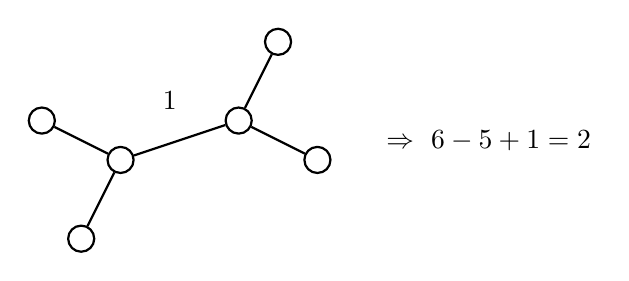
\begin{tikzpicture}[every node/.style={circle, draw=black, thick}, every path/.style={draw=black, thick}]
			\node (a) at (0,0){};
			\node (b) at (-0.5,1.5){};
			\node (c) at (0.5,1){};
			\node (d) at (2,1.5){};
			\node (e) at (2.5,2.5){};
			\node (f) at (3,1){};
			
			\node[draw=white] (f1) at (1.125,1.75){1};
			
			\path (c) edge (b);
			\path (a) edge (c);
			\path (c) edge (d);
			\path (d) edge (e);
			\path (d) edge (f);
			
			\node[rectangle, draw=white] (math) at (5,1.25){$~~~ \Rightarrow ~ 6 - 5 + 1 = 2$};
			\end{tikzpicture}
		\end{center}
		
		\textbf{Переход:} $G$ --- неизвестно. Если $G'$ имеет меньше ребер, то верно. Если $G$ --- не дерево, значит есть цикл. Возьмем любое ребро цикла --- вокруг него точно 2 грани. Теперь удалим это ребро и получим $G'$, $G'$ тоже связен и планарен. Тогда $n'$ --- вершины, $m'$ --- ребра, $f'$ --- грани графа $G'$. Количество вершин не изменилось: $n' = n-1$. Количество ребер и граней стало меньше на 1: $m' = m-1$, $f' = f-1$. Получили:
		$$n'-m'+f'=2 ~~~ \Leftrightarrow ~~~ n - (m - 1) + (f - 1) = n - m + f = 2$$
		
		\begin{center}
			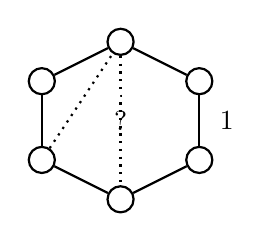
\begin{tikzpicture}[every node/.style={circle, draw=black, thick}, every path/.style={draw=black, thick}]
			\node (a) at (0,0){};
			\node (b) at (0,1){};
			\node (c) at (1,1.5){};
			\node (d) at (2,1){};
			\node (e) at (2,0){};
			\node (f) at (1,-0.5){};
			
			\node[draw=white] (f1) at (2.35,0.5){1};
			
			\path (a) edge (b);
			\path (b) edge (c);
			\path[dotted] (a) edge (c);
			\path (c) edge (d);
			\path (d) edge (e);
			\path (e) edge (f);
			\path (f) edge (a);
			\path[dotted] (c) edge node[draw=white] {?} (f);
			\end{tikzpicture}
		\end{center}
	\end{proof}
	
	\begin{corollary}
		Некоторые следствия из формулы Эйлера:
		\begin{enumerate}
			\item Не важно, как рисовать планарный граф, количество граней постоянно.
			\item Теорема про многогранники. Если взять куб, то по формуле Эйлера: $8-12+6 = 2$
			\begin{center}
				Становится понятно если отобразить куб в виде планарного графа:
				
				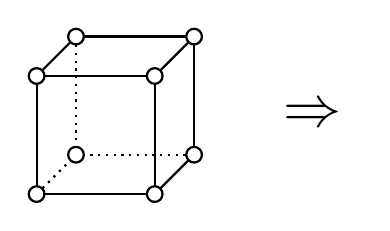
\begin{tikzpicture}[every node/.style={circle, draw=black, thick, scale=0.6}, every path/.style={draw=black, thick}]
				\node (a) at (0,0){};
				\node (b) at (0,1.5){};
				\node (c) at (1.5,1.5){};
				\node (d) at (1.5,0){};
				\node (e) at (0.5,2){};
				\node (f) at (2,2){};
				\node (g) at (2,0.5){};
				\node (h) at (0.5,0.5){};
				
				\path (a) edge (b);
				\path (b) edge (c);
				\path (c) edge (d);
				\path (d) edge (a);
				\path (b) edge (e);
				\path (e) edge (f);
				\path (f) edge (g);
				\path (c) edge (f);
				\path (d) edge (g);
				\path[dotted] (a) edge (h);
				\path[dotted] (e) edge (h);
				\path[dotted] (g) edge (h);
				
				\node[draw = white, rectangle, scale = 3.5] (text) at (3.5, 1){$\Rightarrow$};
				\end{tikzpicture}
				~~~
				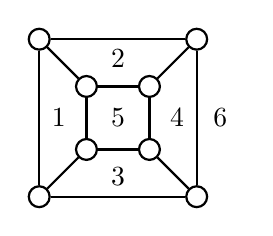
\begin{tikzpicture}[every node/.style={circle, draw=black, thick, scale=0.8}, every path/.style={draw=black, thick}]
				\node (a) at (0,0){};
				\node (b) at (0,2){};
				\node (c) at (2,2){};
				\node (d) at (2,0){};
				\node (e) at (0.6,0.6){};
				\node (f) at (0.6,1.4){};
				\node (g) at (1.4,1.4){};
				\node (h) at (1.4,0.6){};
				
				\path (a) edge (b);
				\path (b) edge (c);
				\path (c) edge (d);
				\path (d) edge (a);
				\path (e) edge (f);
				\path (f) edge (g);
				\path (g) edge (h);
				\path (h) edge (e);
				\path (a) edge (e);
				\path (b) edge (f);
				\path (c) edge (g);
				\path (d) edge (h);
				
				\node[draw = none, scale = 1.25] (f1) at (0.25, 1){1};
				\node[draw = none, scale = 1.25] (f1) at (1, 1.75){2};
				\node[draw = none, scale = 1.25] (f1) at (1, 0.25){3};
				\node[draw = none, scale = 1.25] (f1) at (1.75, 1){4};
				\node[draw = none, scale = 1.25] (f1) at (1, 1){5};
				\node[draw = none, scale = 1.25] (f1) at (2.3, 1){6};
				\end{tikzpicture}
			\end{center}
			\item Если граф $G$ планарен (не обязательно связан), то:
			$$n-m+f = 1+|\text{компоненты связности}|$$
			\item У каждой грани как минимум 3 ребра.
			\begin{proof}
				Посчитаем количество ребер у грани. Можно заметить, что каждое ребро посчитано один или два раза. Тогда:
				$$2m \geq \sum_{f \in \mathbb{F}} |\mathbb{E}|\text{ вокруг }f \geq 3f$$
				
				Следовательно:
				$$3f \leq 2m$$
				
				Тогда:
				$$n - m + f = 2 ~~~~~ (\times 3)$$
				$$3n - 3m + 3f = 6 ~~~ \Leftrightarrow ~~~ 3n - 3m + 2m \geq 6$$
				
				Итого получили, что $m \leq 3n - 6$ в связном планарном графе $G$.
				
				Физический смысл: ребер не может быть очень много.
				\begin{center}
					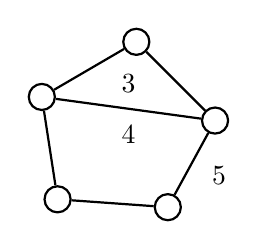
\begin{tikzpicture}[every node/.style={circle, draw=black, thick}, every path/.style={draw=black, thick}]
					\node (a) at (0,0){};
					\node (b) at (-0.2,1.3){};
					\node (c) at (1,2){};
					\node (d) at (2,1){};
					\node (e) at (1.4,-0.1){};
					
					\node[draw=white] (f1) at (2.05,0.3){5};
					
					\path (a) edge (b);
					\path (b) edge (c);
					\path (c) edge (d);
					\path (b) edge node [draw=none, above]{3} node [draw=none, below]{4} (d);
					\path (d) edge (e);
					\path (e) edge (a);
					\end{tikzpicture}
				\end{center}
			\end{proof}
			
			\item Полный граф при $n \geq 5$ не планарен.
			
			\begin{center}
				\begin{tikzpicture}[every node/.style={circle, draw=black, thick}, every path/.style={draw=black, thick}]
				\node (a) at (0,0){};
				\node (b) at (0,1.5){};
				\node (c) at (1.5,1.5){};
				\node (d) at (1.5,0){};
				\node[scale = 0.01, draw = none] (h) at (1.8,1.8){};
				
				\node[draw=white, rectangle] (text) at (0.75,-0.75){граф планарен};
				
				\path (a) edge (b);
				\path (a) edge (c);
				\path (b) edge (c);
				\path (b) edge[bend left = 50] (h);
				\path (h) edge[bend left = 50] (d);
				\path (c) edge (d);
				\path (d) edge (a);
				\end{tikzpicture}
				~~~~~~~~~~~~~~~~
				\begin{tikzpicture}[every node/.style={circle, draw=black, thick}, every path/.style={draw=black, thick}]
				\node (a) at (0,0){};
				\node (b) at (-0.2,1.3){};
				\node (c) at (1,2){};
				\node (d) at (2,1){};
				\node (e) at (1.4,-0.1){};
				
				\node[scale = 0.01, draw=none] (h1) at (1.4,2.4){};
				\node[scale = 0.01, draw=none] (h2) at (-0.4,-0.4){};
				\node[scale = 0.01, draw=none] (h3) at (2.4,1.1){};
				
				\node[draw=white, rectangle] (text) at (1,-1.2){граф не планарен};
				
				\path (a) edge (b);
				\path (b) edge (c);
				\path (b) edge[bend left=46] (h1);
				\path (h1) edge[bend left=46] (d);
				\path (b) edge[bend right=46] (h2);
				\path (h2) edge[bend right=46] (e);
				\path (a) edge (c);
				\path (a) edge (d);
				\path (c) edge (d);
				\path (c) edge[draw = red, very thick, bend left=42] (h3);
				\path (h3) edge[draw = red, very thick, bend left=42] (e);
				\path (d) edge (e);
				\path (e) edge (a);
				\end{tikzpicture}
			\end{center}
			
			\begin{proof}
				Если $n = 5$, то $m = {5 \cdot 4 \over 2} = 10$. Тогда $10 \leq 3 \cdot 5 - 6 = 9$ --- неверно, значит граф не планарен. Любой граф с большим количеством не планарен тем более.
			\end{proof}
		\end{enumerate}
	\end{corollary}
	\begin{remark}
		Пусть $K_5$ --- полный граф с количеством вершин, равным 5. 
	\end{remark}
	
	\begin{proposition}
		Граф $K_{3,3}$ --- тоже не планарен.
		
		\begin{center}
			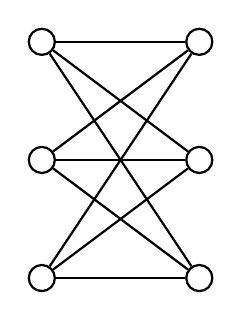
\begin{tikzpicture}[every node/.style={circle, draw=black, thick}, every path/.style={draw=black, thick}]
			\node (a1) at (0,0){};
			\node (a2) at (0,1.5){};
			\node (a3) at (0,3){};
			\node (b1) at (2,0){};
			\node (b2) at (2,1.5){};
			\node (b3) at (2,3){};
			
			\path (a1) edge (b1);
			\path (a1) edge (b2);
			\path (a1) edge (b3);
			\path (a2) edge (b1);
			\path (a2) edge (b2);
			\path (a2) edge (b3);
			\path (a3) edge (b1);
			\path (a3) edge (b2);
			\path (a3) edge (b3);
			\end{tikzpicture}
		\end{center}
	\end{proposition}
	
	\begin{proof}
		В графе $n = 6, m = 9$: $9 \leq 3 \cdot 6 - 6 = 12$ --- сходится.
		
		Рассмотрим количество граней при планарности: $6 - 9 + f$ = 2, следовательно $f = 5$ граней. В $K_{3,3}$ все циклы четные (ход лево-право или право-лево). Следовательно у грани должно быть как минимум 4 ребра.
		$$4f \leq \sum_{f \in \mathbb{F}} |\mathbb{E}|\text{ вокруг }f = 2m$$
		$m$ должно быть хотя бы больше $2f$, но $9 \not{\geq} 2\cdot 5$.
	\end{proof}
	
	\begin{theorem}[Понтрягина-Куратовского]
		Граф $G$ планарен только, если он не содержит подграфов $G_i^\prime$, стягивающихся к $K_5$ и к $K_{3,3}$.
		\begin{note}
			\textit{Стягивающийся к $G$ граф} --- граф $G_1$, похожий на граф $G$ при определенных манипуляциях с ребрами.
		\end{note}
		
		\begin{example}
			Пример стягивающихся графов:
			\begin{center}
				\begin{tikzpicture}[every node/.style={circle, draw=black, thick}, every path/.style={draw=black, thick}]
				\node (a1) at (0,0){};
				\node (a2) at (0,1.5){};
				\node (a3) at (0,3){};
				\node (b1) at (2,0){};
				\node (b2) at (2,1.5){};
				\node (b3) at (2,3){};
				\node (c) at (1,-0.7){};
				
				\node[draw=none, rectangle] (text) at (1,-1.25){стягивается к $K_{3,3}$};
				
				\path (a1) edge (c);
				\path (c) edge (b1);
				\path (a1) edge (b2);
				\path (a1) edge (b3);
				\path (a2) edge (b1);
				\path (a2) edge (b2);
				\path (a2) edge (b3);
				\path (a3) edge (b1);
				\path (a3) edge (b2);
				\path (a3) edge (b3);
				\end{tikzpicture}
				~~~~~~~~~~
				\begin{tikzpicture}[every node/.style={circle, draw=black, thick}, every path/.style={draw=black, thick}]
				\node (a1) at (0.15,0){};
				\node (a2) at (2.85,0){};
				\node (a3) at (3.5,2){};
				\node (a4) at (1.5,3.75){};
				\node (a5) at (-0.5,2){};
				
				\node (b1) at (1,1){};
				\node (b2) at (2,1){};
				\node (b3) at (2.25,1.85){};
				\node (b4) at (1.5,2.5){};
				\node (b5) at (0.75,1.85){};
				
				\node[draw = none, rectangle] (text) at (1.5, -0.5){стягивается к $K_5$};
				
				\path (a1) edge (a2);
				\path (a2) edge (a3);
				\path (a3) edge (a4);
				\path (a4) edge (a5);
				\path (a5) edge (a1);
				
				\path (b1) edge (b3);
				\path (b3) edge (b5);
				\path (b5) edge (b2);
				\path (b2) edge (b4);
				\path (b4) edge (b1);
				
				\path (a1) edge (b1);
				\path (a2) edge (b2);
				\path (a3) edge (b3);
				\path (a4) edge (b4);
				\path (a5) edge (b5);
				\end{tikzpicture}
			\end{center}
		\end{example}
	\end{theorem}
	
	\section{Хроматизм}
	\begin{definition}
		Пусть $G = (\mathbb{V}, \mathbb{E})$ --- граф. \textit{Раскраска графа} $G$ в $k$ цветов это
		$$\text{функция } c: \mathbb{V} \rightarrow \{1 \dots k\}$$
		причем, если есть ребро $(u,v)$, то $c(u) \neq c(v)$. 
	\end{definition}
	
	\begin{example}
		Раскраска графа:
		\begin{center}
			\begin{tikzpicture}[every node/.style={circle, draw=black, thick}, every path/.style={draw=black, thick}]
			\node (a) at (0,0){1};
			\node (b) at (2,0){2};
			\node (c) at (4,0){1};
			\node (d) at (4,2){3};
			\node (e) at (2,2){1};
			\node (f) at (0,2){2};
			
			\node[draw = none, rectangle] (text) at (2, -0.75) {граф раскрашен в 3 цвета};
			
			\path (a) edge (b);
			\path (b) edge (c);
			\path (b) edge (e);
			\path (c) edge (d);
			\path (d) edge (e);
			\path (e) edge (f);
			\path (f) edge (a);
			\end{tikzpicture}
			~~~~~~~~~~
			\begin{tikzpicture}[every node/.style={circle, draw=black, thick}, every path/.style={draw=black, thick}]
			\node (a) at (0,0){3};
			\node (b) at (2,0){2};
			\node (c) at (4,0){1};
			\node (d) at (4,2){3};
			\node (e) at (2,2){2};
			\node (f) at (0,2){1};
			
			\node[draw = none, rectangle] (text) at (2, -0.75) {не раскраска графа};
			
			\path (a) edge (b);
			\path (b) edge (c);
			\path[dashed, very thick] (b) edge node[draw=none, scale=2]{$=$} (e);
			\path (c) edge (d);
			\path (d) edge (e);
			\path (e) edge (f);
			\path (f) edge (a);
			\end{tikzpicture}
		\end{center}
	\end{example}
	
	\begin{problem}
		Какие графы можно раскрасить в 1 цвет?\\
		Ответ: графы без ребер.
	\end{problem}
	
	\begin{problem}
		Какие графы можно раскрасить в 2 цвета?
		\begin{definition}
			Граф $G$ называется \textit{двудольным}, если его можно раскрасить в 2 цвета.
		\end{definition}
		
		\begin{example}
			Двудольные графы:
			\begin{center}
				\begin{tikzpicture}[every node/.style={circle, draw=black, thick}, every path/.style={draw=black, thick}]
				\node (a) at (0,0){1};
				\node (b) at (2,0){2};
				\node (c) at (2,2){1};
				\node (d) at (0,2){2};
				
				\node[draw = none, rectangle] (text) at (1, -0.75) {да};
				
				\path (a) edge (b);
				\path (b) edge (c);
				\path (c) edge (d);
				\path (d) edge (a);
				\end{tikzpicture}
				~~~~~~~~~~~~~~~
				\begin{tikzpicture}[every node/.style={circle, draw=black, thick}, every path/.style={draw=black, thick}]
				\node (a) at (0,0){1};
				\node (b) at (2.5,0){2};
				\node (c) at (1.25,1.75){3};
				
				\node[draw = none, rectangle] (text) at (1.25, -0.75) {нет};
				
				\path (a) edge (b);
				\path (b) edge (c);
				\path (c) edge (a);
				\end{tikzpicture}
			\end{center}
		\end{example}
		
		\begin{note}
			Граф $K_{3,3}$ --- двудолен.
		\end{note}
		\begin{remark}
			Двудольные графы часто рисуют из двух частей (две доли), связанных только в одном направлении (рабочие/задания, студенты/оценки).
			\begin{center}
				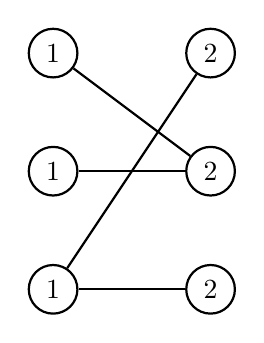
\begin{tikzpicture}[every node/.style={circle, draw=black, thick}, every path/.style={draw=black, thick}]
				\node (a1) at (0,0){1};
				\node (a2) at (0,1.5){1};
				\node (a3) at (0,3){1};
				\node (b1) at (2,0){2};
				\node (b2) at (2,1.5){2};
				\node (b3) at (2,3){2};
				
				\path (a1) edge (b1);
				\path (a1) edge (b3);
				\path (a2) edge (b2);
				\path (a3) edge (b2);
				\end{tikzpicture}
			\end{center}
		\end{remark}
	\end{problem}
	
	\begin{theorem}
		Граф $G$ --- двудолен только, если всего его циклы имеют четную длину.
	\end{theorem}
	
	\begin{proof}[Доказательство четности циклов из двудольности]
		Если бы цикл был нечетный, то конечные цвета будут повторятся, и их нельзя будет соединить. То есть должно быть одинаковое количество разных цветов.
	\end{proof}
	
	\begin{proof}[Доказательство двудольности из четности циклов]
		\char34Подвесим граф за вершину\char34. Тогда эта вершина связана только с вершинами другого цвета. Следующая вершина опять с другим цветом. И так далее, рассматриваем ребра, которые не идут назад --- назначаем цвета по уровням графа в глубину. Почему обратные ребра ничего не портят? Они не соединяют одинаковые цвета, потому что иначе цикл был бы нечетный.
	\end{proof}

	\section{Хроматизм}
	\begin{definition}
		Если $G = (\mathbb{V}, \mathbb{E})$ --- граф, тогда $\chi (G)$ --- \textit{хроматическое число}, то есть минимальное количество цветов, в которые можно раскрасить граф $G$.
	\end{definition}
	\begin{example}
		Примеры расчетов хроматических чисел:
		\begin{center}
			\begin{tikzpicture}[every node/.style={circle, draw=black, thick}, every path/.style={draw=black, thick}]
			\node (a) at (0,2){1};
			\node (b) at (2,2){1};
			\node (c) at (2,0){3};
			\node (d) at (0,0){2};
			
			\node[rectangle, draw=none] (text1) at (-1.5,1.5){Граф $G_1$};
			\node[rectangle, draw=none] (text2) at (1,-0.85){можно раскрасить минимум в 3 цвета};
			\node[rectangle, draw=none, scale=2] (text3) at (9,0.9){$\chi (G_1) = 3$};
			
			\path (b) edge (c);
			\path (c) edge (d);
			\path (d) edge (a);
			\path (d) edge (b);
			\end{tikzpicture}
			
			\begin{tikzpicture}[every node/.style={circle, draw=black, thick}, every path/.style={draw=black, thick}]
			\node (a) at (0,0){2};
			\node (b) at (0,2){1};
			\node (c) at (2,2){2};
			\node (d) at (2,0){1};
			
			\node[draw=white, rectangle] (space) at (0,3.25){};
			\node[rectangle, draw=none] (text1) at (-1.5,1.5){Граф $G_2$};
			\node[rectangle, draw=none] (text2) at (1,-0.85){можно раскрасить минимум в 2 цвета};
			\node[rectangle, draw=none, scale=2] (text3) at (9,0.9){$\chi (G_2) = 2$};
			
			\path (a) edge (b);
			\path (b) edge (c);
			\path (c) edge (d);
			\path (d) edge (a);
			\end{tikzpicture}
		\end{center}
	\end{example}
	\begin{corollary}
		Хроматическое число полного графа $K$ равно количеству его вершин:
		$$\chi (K_{|\mathbb{V}|}) = |\mathbb{V}|$$
	\end{corollary}
	\begin{remark}
		Если $k \geq \chi (G)$, то граф можно раскрасить в $k$ цветов.
	\end{remark}
	
	\begin{proposition*}
		Хроматическое число графа $G$ всегда не больше максимальной степени вершины плюс один.
		$$\chi (G) \leq \max {\deg v} + 1$$
		\begin{center}
			\begin{tikzpicture}[every node/.style={circle, draw=black, thick}, every path/.style={draw=black, thick}]
			\node (a) at (0,1.75){};
			\node (b) at (2,1.75){};
			\node (c) at (4,1.75){};
			\node (d) at (2,-0.25){};
			\node (e) at (4,-0.25){};
			
			\node[rectangle, draw=none] (text1) at (-1.5,1.5){Граф $G$};
			\node[rectangle, draw=none] (text2) at (2,-0.85){$\max \deg v = 4$};
			\node[rectangle, draw=none, scale=2] (text3) at (9.25,0.75){$\chi (G) \leq 4 + 1 = 5$};
			
			\path (a) edge (b);
			\path (a) edge (d);
			\path (b) edge (c);
			\path (b) edge (d);
			\path (c) edge (d);
			\path (d) edge (e);
			\path (a) edge (e);
			\path (d) edge (a);
			\end{tikzpicture}
		\end{center}
	\end{proposition*}
	\begin{proof}
		Индукция по количеству вершин.\\
		\textbf{База.} $n = 0, m = 1$ --- верно, так как $\max {\deg} = 0 \Rightarrow \chi (G) \geq 1$.\\
		\textbf{Переход.} Граф $G$, $v$ --- вершина максимальной степени = $\Delta$. Удаляем ее и получаем подграф $G'$. Максимальная степень подграфа точно не больше степени изначального графа. Попробуем раскрасить в $\Delta + 1$ цвет. Однако цвет запрещен.
		Значит в $\Delta$ цветов раскрасить можно. Продолжая, дойдем то единственной вершины.
		\begin{center}
			\begin{tikzpicture}[every node/.style={circle, draw=black, thick}, every path/.style={draw=black, thick}]
			\node (a) at (0,0){};
			\node (b) at (4,1.5){};
			\node (c) at (4,0.5){};
			\node (d) at (4,-0.5){};
			\node (e) at (4,-1.5){};
			
			\node[draw=none, rectangle,scale=1.75] (text) at (1,-1.25){$\Delta$};
			\node[dashed, rectangle, scale=14.5] (box) at (4,0){};
			\node[draw=none, rectangle, scale=0.8] (boxtext) at (5.15,1.5){Граф $G'$};
			
			\path (a) edge (b);
			\path (a) edge (c);
			\path (a) edge (d);
			\path (a) edge (e);
			\path[->] (text) edge[bend left=30, dotted] (a);
			\end{tikzpicture}
		\end{center}
	\end{proof}
	
	\begin{proposition*}
		Если граф $G$ --- планарный, то его можно раскрасить не более чем в 5 цветов.
	\end{proposition*}
	
	\begin{problem}
		Во сколько цветов достаточно раскрасить страны на географической карте, чтобы любые две соседние не имели один цвет?
		\begin{center}
			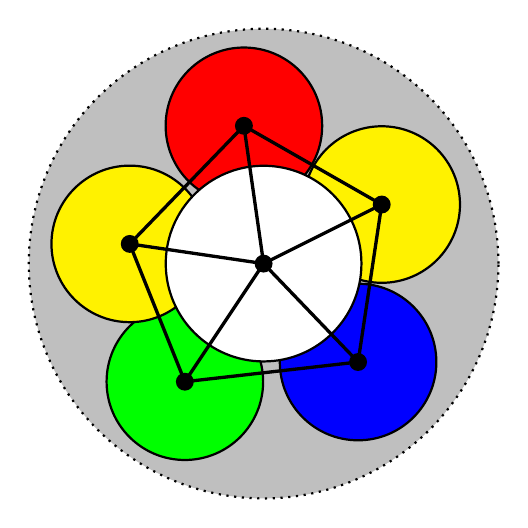
\begin{tikzpicture}[every node/.style={circle, draw=black, thick, scale=6}, every path/.style={draw=black, very thick}]
			\node[dotted, scale=3, fill = lightgray] (g1) at (0,0.25){};
			\node[fill=red] (b1) at (-0.25,2){};
			\node[fill=green] (c1) at (-1,-1.25){};
			\node[fill=yellow] (d1) at (-1.7,0.5){};
			\node[fill=yellow] (e1) at (1.5,1){};
			\node[fill=blue] (f1) at (1.2,-1){};
			\node[scale=1.25, fill=white] (a1) at (0,0.25){};
			
			\node[scale = 0.1, fill=black] (b) at (-0.25,2){};
			\node[scale = 0.1, fill=black] (c) at (-1,-1.25){};
			\node[scale = 0.1, fill=black] (d) at (-1.7,0.5){};
			\node[scale = 0.1, fill=black] (e) at (1.5,1){};
			\node[scale = 0.1, fill=black] (f) at (1.2,-1){};
			\node[scale = 0.1, fill=black] (a) at (0,0.25){};
			
			\path (a) edge (b);
			\path (a) edge (c);
			\path (a) edge (d);
			\path (a) edge (e);
			\path (a) edge (f);
			\path (b) edge (d);
			\path (c) edge (d);
			\path (b) edge (e);
			\path (e) edge (f);
			\path (c) edge (f);
			\end{tikzpicture}
		\end{center}
	\end{problem}
	
	\begin{proof}
		В $G$ есть вершина степени $\leq$ 5.
		Если нет, то все степени $\geq$ 6, значит сумма степеней всех вершин равна хотя бы $6n$ ($n = |\mathbb{V}|$). Мы знаем, что сумма степеней вершин равна удвоенному количеству ребер. Соответственно ребер хотя бы $3m$, однако так не бывает, ведь количество ребер должно быть меньше или равно $3n - 6$.\\\\
		Раскрашиваем в пять цветов по индукции.\\
		\textbf{База.} Графы из 5 вершин точно можно раскрасить в пять цветов.\\
		\textbf{Переход.} Пусть есть граф $G$ с $n > 5$ вершин. Предполагаем, что для него есть раскраска. Берем вершину $v$, у которой степень $\leq 5$. Рассмотрим граф без этой вершины и раскрасим его. Если мы для каждой соседней вершины $v_i$ используем не более четырех цветов, то раскрашиваем ее пятым --- следовательно, для $v$ есть цвет. Если для соседних вершин используются все пять цветов, то снова попробуем убрать вершину из этого графа --- получили одну грань. Возьмем случайные две вершины, не соединенные ребром, и стянем их к $v$ --- получим граф $\tilde G$. Этот граф также остается планарным, при этом у него будет $n-2$ вершины. Значит, две стянутых вершины можно раскрасить в один цвет, следовательно для $v$ также будет цвет.
		
		\begin{center}
			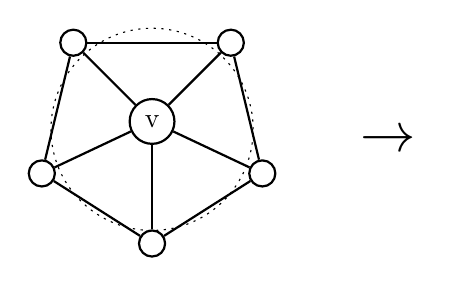
\begin{tikzpicture}[every node/.style={circle, draw=black, thick, fill=white}, every path/.style={draw=black, thick}]
			\node[dotted, thin, scale = 7.75, fill=none] (void) at (0,-0.1){};
			\node (a) at (0,0){v};
			\node (b) at (1,1){};
			\node (c) at (1.4,-0.66){};
			\node (d) at (0,-1.55){};
			\node (e) at (-1.4,-0.66){};
			\node (f) at (-1,1){};
			
			\node[draw=none, rectangle, scale = 2] (arrow) at (3, -0.25){$\rightarrow$};
			
			\path (a) edge (b);
			\path (a) edge (c);
			\path (a) edge (d);
			\path (a) edge (e);
			\path (a) edge (f);
			\path (b) edge (c);
			\path (b) edge (f);
			\path (e) edge (f);
			\path (e) edge (d);
			\path (c) edge (d);
			\end{tikzpicture}
			~~~~
			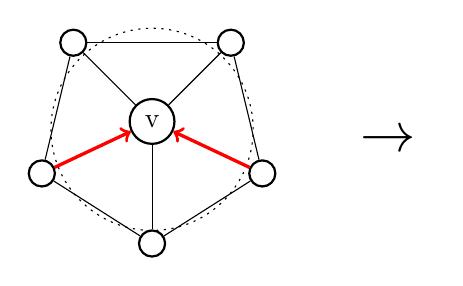
\begin{tikzpicture}[every node/.style={circle, draw=black, thick, fill=white}, every path/.style={draw=black}]
			\node[dotted, thin, scale = 7.75, fill=none] (void) at (0,-0.1){};
			\node (a) at (0,0){v};
			\node (b) at (1,1){};
			\node (c) at (1.4,-0.66){};
			\node (d) at (0,-1.55){};
			\node (e) at (-1.4,-0.66){};
			\node (f) at (-1,1){};
			
			\node[draw=none, rectangle, scale = 2] (arrow) at (3, -0.25){$\rightarrow$};
			
			\path (a) edge (b);
			\path[->] (c) edge[very thick, draw=red] (a);
			\path (a) edge (d);
			\path[->] (e) edge[very thick, draw=red] (a);
			\path (a) edge (f);
			\path (b) edge (c);
			\path (b) edge (f);
			\path (e) edge (f);
			\path (e) edge (d);
			\path (c) edge (d);
			\end{tikzpicture}
			~~~
			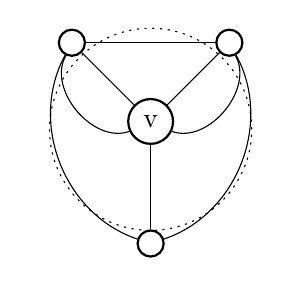
\begin{tikzpicture}[every node/.style={circle, draw=black, thick, fill=white}, every path/.style={draw=black}]
			\node[dotted, thin, scale = 7.75, fill=none] (void) at (0,-0.1){};
			\node (a) at (0,0){v};
			\node (b) at (1,1){};
			\node (d) at (0,-1.55){};
			\node (f) at (-1,1){};
			
			\path (a) edge (b);
			\path (a) edge[bend right = 70] (b);
			\path (a) edge (d);
			\path (a) edge[bend left = 70] (f);
			\path (a) edge (f);
			\path (f) edge[bend right = 50] (d);
			\path (b) edge (f);
			\path (b) edge[bend left = 50] (d);
			\end{tikzpicture}
		\end{center}
		
		\begin{note}
			Между какими-то двумя вершинами точно нет ребра, в другом случае граф будет стягивающимся к $K_5$, то есть он не был бы планарным.
		\end{note}
		\begin{problem}
			Во сколько цветов на самом деле можно раскрасить планарный граф?
			\begin{conjecture}[Проблема 4-ех красок]
				Любой планарный граф можно раскрасить в 4 цвета.
			\end{conjecture}
		\end{problem}
	\end{proof}
	
	\section{Хроматические многочлены}
	\begin{definition}
		Пусть $\chi (G, k)$ --- это функция, которая возвращает количество способов раскраски графа $G$ по $k$ цветам.
	\end{definition}
	\begin{proposition}
		Рассмотрим некоторые функции:
		\begin{enumerate}
			\item Граф без ребер: $\chi (\emptyset_n, k) = k^n$
			\item Полный граф: $\chi (K_n, k) = k(k-1)(k-2)\dots(k-n+1) = {k! \over (k-n)!} = k^{\underline{n}}$
			\item Дерево: $\chi (T_n, k) = k(k-1)^{n-1}$ (по методу подвешивания вершины)
			\item Граф $\overline{G} = (\mathbb{V}, \mathbb{E})$ с каким-то ребром $e = (u,v)$. Граф $G = \overline{G} \backslash e$. Граф $G = G^{\circ}$ --- стянутый в одну вершину.
			Можно заметить, что количество способов раскрасить $G$ в $k$ цветов. Вершины $u$ и $v$ имеют либо одинаковый цвет, либо разный цвет. Если имеют разный цвет, то таких способов столько же, сколько раскрасить $\overline{G}$. Если цвет одинаковый, то столько же, сколько и $G^{\circ}$. То есть:
			$$\chi(G,k) = \chi (\overline{G}, k) + \chi (G^{\circ}, k)$$
			\begin{center}
				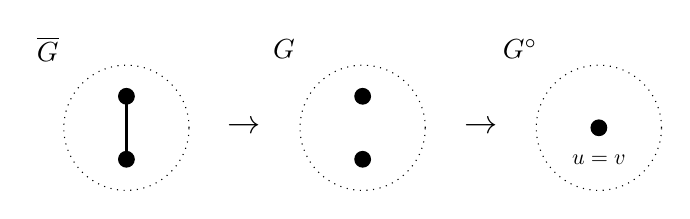
\begin{tikzpicture}[every node/.style={circle, draw=black, fill=black, scale = 0.6}, every edge/.style={draw=black, very thick}]
				\node[dotted, fill=white, scale=8] (field1) at (0,0){};
				\node (a1) at (0,0.4){};
				\node (b1) at (0, -0.4){};
				\node[rectangle, fill=none, draw=none, scale=1.66] (text1) at (-1, 1){$\overline G$};
				
				\path (a1) edge (b1);
				
				\node[rectangle, fill=none, draw=none, scale=2] (arrow1) at (1.5,0){$\rightarrow$};
				
				\node[dotted, fill=white, scale=8] (field2) at (3,0){};
				\node (a2) at (3,0.4){};
				\node (b2) at (3, -0.4){};
				\node[rectangle, fill=none, draw=none, scale=1.66] (text2) at (2, 1){$G$};
				
				\node[rectangle, fill=none, draw=none, scale=2] (arrow2) at (4.5,0){$\rightarrow$};
				
				\node[dotted, fill=white, scale=8] (field3) at (6,0){};
				\node (a3) at (6,0){};
				\node[rectangle, fill=none, draw=none, scale=1.66] (text3) at (5, 1){$G^\circ$};
				\node[rectangle, fill=none, draw=none, scale=1.33] (text31) at (6, -0.4){$u=v$};
				\end{tikzpicture}
			\end{center}
			\begin{corollary}[к пункту 4]
				Обратное условие:
				$$\chi (\overline{G}, k) = \chi(G,k) - \chi (G^{\circ}, k)$$
				\begin{center}
					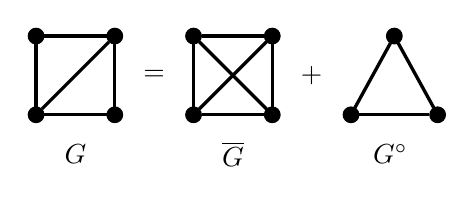
\begin{tikzpicture}[every node/.style={circle, draw=black, fill=black, scale = 0.6}, every edge/.style={draw=black, very thick}]
					\node (a1) at (0,0){};
					\node (a2) at (0,1){};
					\node (a3) at (1,1){};
					\node (a4) at (1,0){};
					
					\path (a1) edge (a2);
					\path (a2) edge (a3);
					\path (a3) edge (a4);
					\path (a4) edge (a1);
					\path (a1) edge (a3);
					
					\node[rectangle, draw=none, fill=none, scale=1.66] (equal) at (1.5,0.5){$=$};
					
					\node (b1) at (2,0){};
					\node (b2) at (2,1){};
					\node (b3) at (3,1){};
					\node (b4) at (3,0){};
					
					\path (b1) edge (b2);
					\path (b2) edge (b3);
					\path (b3) edge (b4);
					\path (b4) edge (b1);
					\path (b1) edge (b3);
					\path (b2) edge (b4);
					
					\node[rectangle, draw=none, fill=none, scale=1.66] (plus) at (3.5,0.5){$+$};
					
					\node (c1) at (4,0){};
					\node (c2) at (4.55,1){};
					\node (c3) at (5.1,0){};
					
					\path (c1) edge (c2);
					\path (c2) edge (c3);
					\path (c3) edge (c1);
					
					\node[rectangle, draw=none, fill=none, scale=1.66] (text1) at (0.5,-0.5){$G$};
					\node[rectangle, draw=none, fill=none, scale=1.66] (text2) at (2.5,-0.5){$\overline{G}$};
					\node[rectangle, draw=none, fill=none, scale=1.66] (text3) at (4.5,-0.5){$G^\circ$};
					\end{tikzpicture}
					$\chi(\overline{G},k)= k(k-1)(k-2)(k-3) + k(k-1)(k-2) = k(k-1)(k-2)^2$
				\end{center}
			\end{corollary}
			\item Цикл: $\chi (C_n, k) = \chi (T_n, k) - \chi (C_{n-1}, k) = \chi (T_n, k) - \chi (T_{n-1}, k) + \chi (C_{n-2}, k) = \dots$ --- останавливаемся на цикле длиной три, иначе не получим цикл. В финале получим сумму, являющуюся геометрической прогрессией с шагом $1-k$ и первым членом $(-1)^n \cdot k(k-1)$:
			$$\chi (C_n, k) = k(k-1)^{n-1} - k(k-1)^{n-2} + \cdots \pm k(k-1) \pm k = (k-1)^n - (-1)^n$$
		\end{enumerate}
	\end{proposition}
	
	\begin{proposition}
		Пусть есть граф $G$ и он имеет висячую вершину $v$, и $G' = G \backslash v$. Тогда:
		$$\chi (G, k) = \chi (G', k) \cdot (k-1)$$
	\end{proposition}
	\begin{center}
		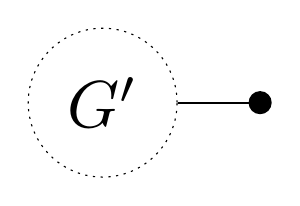
\begin{tikzpicture}[every node/.style={circle, draw=black, fill=black, thick, scale=0.8}, every edge/.style={draw=black, thick}]
		\node[fill=none, dotted, thin, scale=3] (a) at (0,0){$G'$};
		\node (b) at (2,0){};
		
		\path (a) edge (b);
		\end{tikzpicture}
	\end{center}
	
	\begin{proposition}
		Если в графе $G$ есть вершина $v$, образующая треугольник с двумя случайными вершинами, то:
		$$\chi (G, k) = \chi(G', k)\cdot(k-2)$$
	\end{proposition}
	\begin{center}
		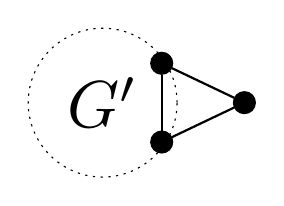
\begin{tikzpicture}[every node/.style={circle, draw=black, fill=black, thick, scale=0.8}, every path/.style={draw=black, thick}]
		\node[fill=none, dotted, thin, scale=3] (G) at (0,0){$G'$};
		\node (a) at (0.75,0.5){};
		\node (b) at (1.8,0){};
		\node (c) at (0.75,-0.5){};
		
		\path (a) edge (b);
		\path (c) edge (b);
		\path (a) edge (c);
		\end{tikzpicture}
	\end{center}
	
	\begin{proposition}
		Пусть $G = G'_1 \cup G'_2$, при этом отсутствуют ребра между $G'_1$ и $G'_2$. Тогда:
		$$\chi (G, k) = \chi (G'_1, k)\cdot \chi (G'_2, k)$$
	\end{proposition}
	\begin{center}
		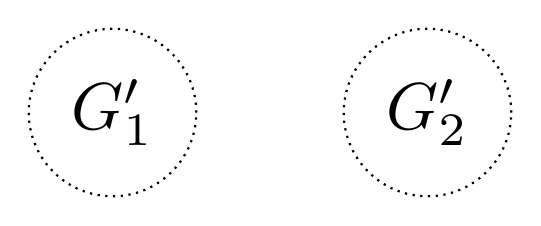
\begin{tikzpicture}[every node/.style={circle, draw=black, dotted, scale=2.4}, every path/.style={draw=black, thick}]
		\node (G1) at (0,0){$G'_1$};
		\node (G2) at (4,0){$G'_2$};
		\end{tikzpicture}
	\end{center}
	
	\begin{example}
		Рассмотрим преобразование графа $G$. Красные вершины удаляются:
		\begin{center}
			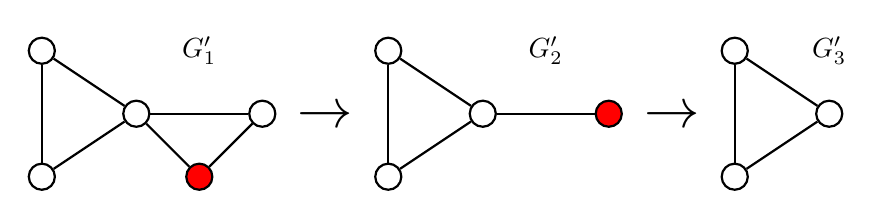
\begin{tikzpicture}[every node/.style={circle, draw=black, thick}, every edge/.style={draw=black, thick}]
			\node (a1) at (0,0){};
			\node (b1) at (0,-1.6){};
			\node (c1) at (1.2,-0.8){};
			\node (d1) at (2.8,-0.8){};
			\node (e1)[fill=red] at (2,-1.6){};
			\node[rectangle, draw=none] (text1) at (2,0){$G'_1$};
			
			\node[rectangle, draw=none, scale=2] (arrow1) at (3.6,-0.85){$\rightarrow$};
			
			\path (a1) edge (b1);
			\path (c1) edge (b1);
			\path (c1) edge (a1);
			\path (c1) edge (d1);
			\path (c1) edge (e1);
			\path (e1) edge (d1);
			
			\node (a2) at (4.4,0){};
			\node (b2) at (4.4,-1.6){};
			\node (c2) at (5.6,-0.8){};
			\node (d2)[fill=red] at (7.2,-0.8){};
			\node[rectangle, draw=none] (text2) at (6.4,0){$G'_2$};
			
			\node[rectangle, draw=none, scale=2] (arrow2) at (8,-0.85){$\rightarrow$};
			
			\path (a2) edge (b2);
			\path (c2) edge (b2);
			\path (c2) edge (a2);
			\path (c2) edge (d2);
			
			\node (a3) at (8.8,0){};
			\node (b3) at (8.8,-1.6){};
			\node (c3) at (10,-0.8){};
			\node[rectangle, draw=none] (text) at (10,0){$G'_3$};
			
			\path (a3) edge (b3);
			\path (c3) edge (b3);
			\path (c3) edge (a3);
			\end{tikzpicture}
			$$\chi(G'_1, k) = \chi(G'_2, k)(k-2) = \chi(G'_3, k)(k-1)(k-2) = k(k-1)^2(k-2)^2$$
		\end{center}
	\end{example}
	
	\begin{proposition}
		$\chi (G, k)$ --- хроматический многочлен, обладающий данными свойствами:
		\begin{enumerate}
			\item Старший коэффициент всегда равен 1;
			\item Степень многочлена = $n$ (количество вершин = $n$);
			\item Знаки многочлена всегда чередуются;
			\item Младший коэффициент всегда равен 0;
			\item Количество ребер графа $G$ равно абсолютному значению коэффициента при $k^{n-1}$.
		\end{enumerate}
	\end{proposition}
	
	\begin{proof}
		Индукция по количеству вершин.\\
		\textbf{База.} Рассматриваем пустой граф из $n$ вершин: $\chi (\emptyset, k) = k^n$ --- это действительно многочлен, удовлетворяющий всем свойствам.\\
		\textbf{Переход.} Пусть есть граф с $m$ ребер. Рассмотрим следующий пример:
		\begin{center}
			\begin{tikzpicture}[every node/.style={circle, draw=black, fill=black, scale=0.5}, every edge/.style={draw=black, thick}]
			\node[scale=6.4, dotted, fill=none] (field1) at (0,0){};
			\node (a1) at (-0.25,0){};
			\node (b1) at (0.2,0.2){};
			\node (c1) at (0.2,-0.2){};
			
			\path (a1) edge (b1);
			
			\node[scale=6.4, dotted, fill=none] (field1) at (-4.05,0){};
			\node (a2) at (-4.3,0){};
			\node (b2) at (-3.85,0.2){};
			\node (c2) at (-3.85,-0.2){};
			
			\path (a2) edge (b2);
			\path (b2) edge (c2);
			
			\node[scale=6.4, dotted, fill=none] (field1) at (3.95,0){};
			\node (a1) at (3.95,0){};
			
			\node[rectangle, scale=3.6, fill=none, draw=none] (math) at (0.12,0){$\chi(~~~~~, k) = \chi(~~~~~, k) - \chi(~~~~~, k)$};
			\end{tikzpicture}
		\end{center}
		Ребер стало меньше. Рассмотрим свойства:
		\begin{enumerate}
			\item Коэффициент остался: $1 \cdot k^n - k^{n-1} + \cdots$;
			\item Степень осталась $n$ --- следует из предыдущего;
			\item Знаки чередуются: $k^n - (k^{n-1} - k^{n-2} - \cdots) + \cdots = k^n - k^{n-1} + k^{n-2} + \cdots$;
			\item Младший коэффициент: $0 - 0 = 0$;
			\item Количество ребер: $-\text{ребра} \cdot k^{n-1} - k^{n-1} = -k^{n-1}\cdot(\text{ребра}+1)$.
		\end{enumerate}
	\end{proof}
	
	\begin{proposition}
		Хроматическое число многочлена $\chi (G)$ равно первому значению корня многочлена, при котором не получается ноль.
	\end{proposition}
	
	\section{Эйлеровы графы}
	\begin{problem}
		Нарисовать данный граф, не проводя по одному ребру дважды:
		\begin{center}
			\begin{tikzpicture}[every node/.style={circle, draw=black, thick}, every edge/.style={draw=black, thick}]
			\node (a) at (0,0){};
			\node (b) at (-1,-1.5){};
			\node (c) at (1,-1.5){};
			\node (d) at (-1,-3.5){};
			\node (e) at (1,-3.5){};
			
			\path (a) edge (b);
			\path (b) edge (c);
			\path (a) edge (c);
			\path (c) edge (e);
			\path (c) edge (d);
			\path (b) edge (e);
			\path (b) edge (d);
			\path (e) edge (d);
			\end{tikzpicture}
		\end{center}
	\end{problem}
	
	\begin{definition}
		\textit{Эйлеров путь} --- простой путь, содержащий все ребра.
	\end{definition}
	
	\begin{definition}
		\textit{Эйлеров цикл} --- цикл, содержащий все ребра.
	\end{definition}
	
	\begin{proposition}
		Пусть $G$ содержит эйлеров цикл, тогда $G$ связен, и $\deg v$ --- четная $\forall v \in \mathbb{V}$. 
	\end{proposition}
	
	\begin{center}
		\begin{tikzpicture}[every node/.style={circle, draw=black, thick}, every edge/.style={draw=black, thick}]
		\node (a1) at (0,-0.55){2};
		\node (b1) at (-1,-2){4};
		\node (c1) at (1,-2){4};
		\node (d1) at (-1,-4){3};
		\node (e1) at (1,-4){3};
		
		\path (a1) edge (b1);
		\path (b1) edge (c1);
		\path (a1) edge (c1);
		\path (c1) edge (e1);
		\path (c1) edge (d1);
		\path (b1) edge (e1);
		\path (b1) edge (d1);
		\path (e1) edge (d1);
		
		\node (a2) at (5,0){2};
		\node (b2) at (4,-1.5){4};
		\node (c2) at (6,-1.5){4};
		\node (d2) at (4,-3.5){4};
		\node (e2) at (6,-3.5){4};
		\node (f2) at (5,-5){2};
		
		\path (a2) edge (b2);
		\path (b2) edge (c2);
		\path (a2) edge (c2);
		\path (c2) edge (e2);
		\path (c2) edge (d2);
		\path (b2) edge (e2);
		\path (b2) edge (d2);
		\path (e2) edge (d2);
		\path (e2) edge (f2);
		\path (f2) edge (d2);
		
		\node[rectangle, draw=none] (text1) at (0,0.2){нет циклов};
		\node[rectangle, draw=none] (text2) at (5,0.7){есть цикл};
		\end{tikzpicture}
	\end{center}
	
	\begin{proof}[Прямое доказательство]
		Если граф $G$ связен, то до каждой вершины можно дойти. Мы в нее вошли и вышли одинаковое количество раз, соответственно в любом случае степень такой вершины будет четной.
	\end{proof}
	\begin{proof}[Обратное доказательство]
		Начнем строить цикл. Идем из любой вершины, выбираем ребро, которое еще не использовалось. Вершину мы могли посещать до этого, то есть мы пришли в нее, и вышли одинаковое количество раз. Пусть мы в нее пришли еще раз, получим нечетную степень. Следовательно должно быть еще одно ребро, а если мы застряли, то мы из этой вершины начали (ведь вышли из нее только один раз). Итого, каждая степень четная.
	\end{proof}
	\begin{center}
		\begin{tikzpicture}[every node/.style={circle, thick}, every edge/.style={draw=black, thick}, every path/.style={->}]
		\node[draw=black, scale=1.5] (center) at (0,0){};
		\node (a) at (-1.5,1.2){};
		\node (b) at (-2,0){};
		\node (c) at (-1.5,-1.2){};
		\node (d) at (1.5,1.2){};
		\node (e) at (2,0){};
		\node (f) at (1.5,-1.2){};
		
		\path (center) edge (d);
		\path (center) edge (e);
		\path (center) edge[draw=red] (f);
		\path (a) edge[draw=green] (center);
		\path (b) edge (center);
		\path (c) edge (center);
		\end{tikzpicture}
	\end{center}
	
	\begin{remark}
		Если есть два цикла в одной вершине, то их можно объединить:
		\begin{center}
			\begin{tikzpicture}[every node/.style={circle, draw=black, fill=black, scale=0.5}, every edge/.style={draw=black, thick}]
			\node[fill=none, scale=2, very thick] (v) at (0,0){};
			\node (a) at (1, -2){};
			\node (b) at (-2,-1.2){};
			\node (c) at (-1, 0.7){};
			
			\node (d) at (1, 1){};
			\node (e) at (2,-0.8){};
			\node (f) at (-0.1, -0.8){};
			
			\path[->] (v) edge[bend left=50] node[rectangle, right, fill=none, draw=none, scale = 1.5]{4} (a);
			\path[->] (a) edge[bend left=50] (b);
			\path[->] (b) edge[bend left=60] (c);
			\path[->] (c) edge[bend left=30] node[rectangle, right, fill=none, draw=none, scale = 1.5]{1} (v);
			
			\path[->] (v) edge[bend left=30] node[rectangle, left, fill=none, draw=none, scale = 1.5]{2} (d);
			\path[->] (d) edge[bend left=60] (e);
			\path[->] (e) edge[bend left=40] (f);
			\path[->] (f) edge[bend left=45] node[rectangle, left, fill=none, draw=none, scale = 1.5]{3} (v);
			\end{tikzpicture}
		\end{center}
	\end{remark}
	
	\begin{theorem}
		Граф $G$ содержит эйлеров путь, если он связен, а также если степени всех вершин четные, или степени любых двух из них нечетные, а все остальные четные.
	\end{theorem}
	
	\begin{note}
		Необходимо начать эйлеров путь из одной из нечетных вершины, при этом концом должна быть вторая вершина.
	\end{note}
	
	\begin{definition}
		\textit{Гамильтонов путь/цикл} --- простая цепь/цикл по всем вершинам, не повторяясь.
	\end{definition}
	
	\begin{example}
		Примеры гамильтоновых пути и цикла:
		\begin{center}
			\begin{tikzpicture}[every node/.style={circle, draw=black, scale=0.75, very thick}, every edge/.style={draw=black, dashed}]
			\node (a) at (0,0){a};
			\node (b) at (0.2,1){b};
			\node (c) at (1.2,0.3){c};
			\node (d) at (2.4,0.6){d};
			\node (e) at (2.2,-0.4){e};
			
			\path[->] (a) edge[very thick, solid] (b);
			\path (a) edge (c);
			\path[->] (b) edge[very thick, solid] (c);
			\path[->] (d) edge[very thick, solid] (e);
			\path (c) edge (e);
			\path[->] (c) edge[very thick, solid] (d);
			
			\node[rectangle, draw=none, scale=1.25] (text) at (1.2, -1){$abcde$ --- гамильтонов путь};
			\end{tikzpicture}
			~~~~~~~~~~~
			\begin{tikzpicture}[every node/.style={circle, draw=black, scale=0.75, very thick}, every edge/.style={draw=black, very thick}]
			\node (a) at (0.8,-0.2){a};
			\node (b) at (-0.8,-0.75){b};
			\node (c) at (-2,0.2){c};
			\node (d) at (-3.5,0.7){d};
			\node (e) at (-3.9,-0.9){e};
			\node (f) at (-2.4,-1.2){f};
			\node (g) at (0.4,-1.5){g};
			\node[rectangle, draw=none, scale=1.25] (text) at (-1.4, -2.1){$abcdefga$ --- гамильтонов цикл};
			
			\path[->] (a) edge (b);
			\path[->] (b) edge (c);
			\path[->] (c) edge (d);
			\path[->] (d) edge (e);
			\path[->] (e) edge (f);
			\path[->] (f) edge (g);
			\path[->] (g) edge (a);
			\path (a) edge[thin, dashed, bend right=40] (d);
			\path (d) edge[thin, dashed] (f);
			\path (f) edge[thin, dashed] (b);
			\path (b) edge[thin, dashed] (g);
			\path (c) edge[thin, dashed] (f);
			\end{tikzpicture}
		\end{center}
	\end{example}

	\section{Длина, диаметр, радиус}
	\begin{definition}
		\textit{Длина пути} в графе $G$ --- это количество ребер в пути.
	\end{definition}
	\begin{example}
		Рассмотрим следующий пример:
		\begin{center}
			\begin{tikzpicture}[every node/.style={circle, draw=black, thick}, every edge/.style={draw=black, thick}]
			\node (a) at (0,0){a};
			\node (b) at (1.2,0.5){b};
			\node (c) at (1.2,-0.5){c};
			\node (d) at (2.4,0){d};
			\node (e) at (2.4,-1){e};
			\node (f) at (3.6,0-0.5){f};
			
			\path (a) edge (b);
			\path (a) edge (c);
			\path (c) edge (b);
			\path (c) edge (d);
			\path (d) edge (e);
			\path (d) edge (f);
			\path (c) edge (e);
			
			\node[rectangle, draw = none] (text1) at (7,0.7){путь от $a$ до $f$:};
			\node[rectangle, draw = none] (text2) at (7,0.2){$abcdf$ --- длина 4};
			\node[rectangle, draw = none] (text3) at (7,-0.3){$acrdf$ --- длина 4};
			\node[rectangle, draw = none] (text4) at (7,-0.8){$acdf$ --- длина 3};
			\node[rectangle, draw = none] (text5) at (7,-1.3){$abcedf$ --- длина 5};
			\end{tikzpicture}
		\end{center}
	\end{example}
	
	\begin{definition}
		\textit{Расстоянием между вершинами} $d(u,v)$ называется минимальная длина пути между вершинами $u$ и $v$. Частный случай, длина равна $+\infty$, если пути между этими вершинами не существует.
	\end{definition}
	\begin{example}
		Из предыдущего примера: $d(a,f) = 3$.
	\end{example}
	
	\begin{definition}
		\textit{Диаметром графа} называется максимальное расстояние между вершинами графа.
	\end{definition}
	\begin{example}
		В примере выше: расстояние $d(a,f)$ является максимальным, следовательно диаметр графа $G$ = 3.\\
		Еще один пример:
		\begin{center}
			\begin{tikzpicture}[every node/.style={circle, draw=black, thick}, every edge/.style={draw=black, very thick, dashed}]
			\node (a) at (0,0){};
			\node (b) at (0,1.5){};
			\node[fill = blue] (c) at (0,3){};
			\node (d) at (1.5,0){};
			\node (e) at (1.5,1.5){};
			\node (f) at (1.5,3){};
			\node[fill = blue] (g) at (3,0){};
			\node (h) at (3,1.5){};
			\node (i) at (3,3){};
			
			\path (a) edge (b);
			\path (b) edge (c);
			\path (d) edge (e);
			\path (e) edge[draw = blue, solid] (f);
			\path (g) edge[draw = blue, solid] (h);
			\path (h) edge (i);
			\path (a) edge (d);
			\path (d) edge (g);
			\path (b) edge (e);
			\path (e) edge[draw = blue, solid] (h);
			\path (c) edge[draw = blue, solid] (f);
			\path (f) edge (i);
			
			\node[rectangle, draw=none] (text) at (5.5,1.5){--- диаметр 4};
			\end{tikzpicture}
		\end{center}
		Заметим, что остальные расстояния (\textbf{важно --- НЕ пути}) $\leq 4$.
	\end{example}
	
	\begin{definition}
		Для каждой вершины графа $G=(\mathbb{V}, \mathbb{E})$ можно посчитать максимальное расстояние до других вершин. Обозначим это \textit{радиусом вершины}:
		$$r(v) = \max{\{d(u,v)~|~u \in \mathbb{V}\}}$$
		Тогда, \textit{радиусом графа} является минимальное значений $r(v)$:
		$$r(G) = \min{\{r(v)~|~v \in \mathbb{V}\}}$$
	\end{definition}
	\begin{definition}
		Вершины с минимальным радиусом называют \textit{центрами графа}.
	\end{definition}
	\begin{example}
		Из прошлого примера:
		\begin{center}
			\begin{tikzpicture}[every node/.style={circle, draw=black, thick}, every edge/.style={draw=black, thick}]
			\node (a) at (0,0){4};
			\node (b) at (0,2){3};
			\node (c) at (0,4){4};
			\node (d) at (2,0){3};
			\node[fill=black, text=white] (e) at (2,2){2};
			\node (f) at (2,4){3};
			\node (g) at (4,0){4};
			\node (h) at (4,2){3};
			\node (i) at (4,4){4};
			
			\path (a) edge (b);
			\path (b) edge (c);
			\path (d) edge (e);
			\path (e) edge (f);
			\path (g) edge (h);
			\path (h) edge (i);
			\path (a) edge (d);
			\path (d) edge (g);
			\path (b) edge (e);
			\path (e) edge (h);
			\path (c) edge (f);
			\path (f) edge (i);
			\end{tikzpicture}
		\end{center}
		Таким образом, радиус графа $r(G) = \min{\{4,3,4,3,2,3,4,3,4\}} = 2$. Центр помечен черным цветом.
	\end{example}
	
	\begin{note}
		Центров графа может быть несколько.
		\begin{center}
			\begin{tikzpicture}[every node/.style={circle, draw=black, thick, scale=0.8}, every edge/.style={draw=black, thick}]
			\node (a) at (0,0){3};
			\node[fill=black, text = white] (b) at (2,0){2};
			\node[fill=black, text = white] (c) at (4,0){2};
			\node (d) at (6,0.2){3};
			\node (e) at (5.6, -0.85){3};
			
			\node[rectangle, draw=none, scale=1.25] (text) at (2.75, -1.2){$r(G) \geq 2$, 2 центра};
			
			\path (a) edge (b);
			\path (b) edge (c);
			\path (c) edge (d);
			\path (c) edge (e);
			\end{tikzpicture}
		\end{center}
	\end{note}
	
	\begin{proposition}
		В любом графе $G = (\mathbb{V}, \mathbb{E})$ $d(G) \leq 2r(G)$.
	\end{proposition}
	\begin{proof}
		Пусть $c$ --- центр графа, $c,u,v \in \mathbb{V}$.
		\begin{center}
			\begin{tikzpicture}[every node/.style={circle, draw=black, thick}, every edge/.style={draw=black, thick, dashed}]
			\node (a) at (0,0){$u$};
			\node (b) at (2,0){$c$};
			\node (c) at (4,0){$v$};
			
			\path (a) edge[bend left=25] node[below, draw =none, rectangle, scale=0.75] {$\leq r$}(b);
			\path (b) edge[bend right=25] node[above, draw=none, rectangle, scale = 0.75]{$\leq r$} (c);
			\end{tikzpicture}
		\end{center}
		Заметим, что $d(c,u) \leq r(G),~d(c,v) \leq r(G)$, следовательно по транзитивности $d(u,v) = d(c,u)+d(c,v) \leq 2r(G)$. При этом максимум среди двух вершин $d(u,v)$ также $\leq 2r(G)$.
	\end{proof}
	
	\begin{proposition}
		В дереве может быть не более двух центров.
	\end{proposition}
	\begin{proof}[Доказательство от обратного]
		Пусть центров в дереве 3 : $\{c_1, c_2, c_3\}$. Построим пути между $c_1$ и $c_2$, а затем между $c_2$ и $c_3$ (вспоминая, что в дереве может быть только один путь).
		\begin{center}
			\begin{tikzpicture}[every node/.style={circle, draw=black, thick, scale=0.8}, every edge/.style={draw=black}]
			\node (a) at (0,0){$c_1$};
			\node (b) at (3,0){$c_2$};
			\node (c) at (6,0){$c_3$};
			
			\node[scale=0.33, fill = black] (a1) at (1, 0.5){};
			\node[scale=0.33, fill = black] (b1) at (2, -0.5){};
			
			\node[scale=0.33, fill = blue, draw = blue] (b2) at (4, 0.5){};
			\node[scale=0.33, fill = blue, draw = blue] (c1) at (5, -0.5){};
			
			\path (a) edge[dotted, thick] (b);
			\path (c) edge[dotted, thick] (b);
			\path (a) edge (a1);
			\path (a1) edge (b1);
			\path (b1) edge (b);
			\path (b) edge[draw = blue] (b2);
			\path (b2) edge[draw = blue] (c1);
			\path (c1) edge[draw = blue] (c);
			\end{tikzpicture}
		\end{center}
		Если оба полученных пути проходят через одну вершину \char34развилка\char34 $c_0$, то ее радиус меньше остальных центров.
		$$r(c_0)<r(c_1)=r(c_2)=r(c_3)=r(G)$$
		Следовательно, на самом деле, вершина $c_0$ является центром, а $r(G) = r(c_0)$, что значит, что центров не 3, а уже 1. Пришли к противоречию.
	\end{proof}
	\begin{proof}[Условное доказательство]
		Еще один вариант доказательства: удалим \textit{листья} дерева (висячие вершины) и получим дерево, в котором все оставшиеся расстояния уменьшились на единицу. Соответственно, так как уменьшились все расстояния, то центр (или центры) не изменились. Продолжая удалять снова висячие вершины, мы дойдем до дерева, в котором останется одна или две вершины. Соответственно, эти вершины и будут центрами.
	\end{proof}
	
	\section{Утверждения про ориентированные графы}
	\begin{remark}
		Далее иногда будут использоваться ориентированные графы.
	\end{remark}
	
	\begin{definition}
		В ориентированном графе (\textit{орграфе}) $G = (\mathbb{V}, \mathbb{E})$ множество ребер $\mathbb{E}$ является множеством упорядоченных пар.
	\end{definition}
	\begin{note}
		Ребра в ориентированных графах часто называют дугами.
	\end{note}
	
	\begin{example}
		Ориентированный граф:
		\begin{center}
			\begin{tikzpicture}[every node/.style={circle, draw=black, thick}, every edge/.style={draw=black, thick}, every path/.style = {->}]
			\node (a) at (0,0){};
			\node (b) at (0.7,1.5){};
			\node (c) at (2,1.5){};
			\node (d) at (2,0){};
			
			\path (a) edge (b);
			\path (a) edge (c);
			\path (b) edge (c);
			\path (a) edge[bend right=10] (d);
			\path (d) edge[bend right=10] (a);
			\path (d) edge (c);
			\end{tikzpicture}
		\end{center}
	\end{example}
	
	\begin{remark}
		Существует \textit{взвешенный граф} --- такой граф $G = (\mathbb{V}, \mathbb{E})$, в котором у каждого ребра есть \textit{вес}, то есть функция $f$, которая сопоставляет ребрам $e \in \mathbb{E}$ вещественное число $a \in \mathbb{R}$.
		
		\begin{center}
			\begin{tikzpicture}[every node/.style={circle, draw=black, thick}, every edge/.style={draw=black, thick}]
			\node (a) at (0,0){};
			\node (b) at (2,0){};
			\node (c) at (1,1.5){};
			
			\path (a) edge node[below, rectangle, draw=none, scale=0.75]{$1$} (b);
			\path (a) edge node[left, rectangle, draw=none, scale=0.75]{$2$}(c);
			\path (b) edge node[right, rectangle, draw=none, scale=0.75]{$5$}(c);
			
			\node[rectangle, draw = none] (text) at (3, 0.75){или};
			
			\node (d) at (4,0){};
			\node (e) at (5.8,-0.25){};
			\node (f) at (5.3,1.3){};
			
			\path[->] (f) edge node[right, rectangle, draw=none, scale=0.75]{$2$} (e);
			\path[->] (d) edge[bend left=10] node[above, rectangle, draw=none, scale=0.75]{$3$}(e);
			\path[->] (e) edge[bend left=30] node[below, rectangle, draw=none, scale=0.75]{$4$}(d);
			\path[->] (d) edge node[left, rectangle, draw=none, scale=0.75]{$1$}(f);
			
			\end{tikzpicture}
		\end{center}
	\end{remark}
	
	\begin{definition}
		Расстояние на графе с весами считается как минимальная сумма весов по всем путям.
		$$d = \min{\sum_{i}^{|\mathbb{E}|} a_i}$$
		
		\begin{example}
			Рассмотрим следующий ориентированный граф и найдем расстояние от $a$ до $b$:
			\begin{center}
				\begin{tikzpicture}[every node/.style={circle, draw=black, thick}, every edge/.style={draw=black, thick}]
				\node (a) at (0,0){a};
				\node (c) at (1.5,1){c};
				\node (e) at (1.5,-1){e};
				\node (d) at (3.5,1){d};
				\node (f) at (3.5,-1){f};
				\node (b) at (5,0){b};
				
				\path (a) edge node[rectangle, draw=none, scale=0.75, above]{1} (c);
				\path (a) edge node[rectangle, draw=none, scale=0.75, below]{2} (e);
				\path (c) edge node[rectangle, draw=none, scale=0.75, above]{4} (d);
				\path (e) edge node[rectangle, draw=none, scale=0.75, below]{1} (f);
				\path (e) edge node[rectangle, draw=none, scale=0.75, above left]{3} (d);
				\path (d) edge node[rectangle, draw=none, scale=0.75, above]{2} (b);
				\path (f) edge node[rectangle, draw=none, scale=0.75, below]{5} (b);
				\end{tikzpicture}
				~~~~~
				\begin{tikzpicture}
				\node (a) at (0,0){$d(acdb) = 1 + 4 + 2 = 7$};
				\node (b) at (0,-0.5){$d(acdefb) = 1 + 4 + 3 + 1 + 5 = 14$};
				\node (c) at (0,-1){$d(aefb) = 2 + 1 + 5 = 8$};
				\node (d) at (0,-1.5){$d(aedb) = 2 + 3 + 2 = 7$};
				
				\node (d) at (0,-2.25){$d(a,b) = 7$};
				\end{tikzpicture}
			\end{center}
			\textbf{Ответ:} $d(a,b) = 7$.
		\end{example}
	\end{definition}
	
	\begin{remark}
		Расстояние во взвешенном графе не всегда удается посчитать.
		\begin{example}
			Рассмотрим следующий ориентированный граф и найдем расстояние от $a$ до $b$:
			\begin{center}
				\begin{tikzpicture}[every node/.style={circle, draw=black, thick}, every edge/.style={draw=black, thick}, every path/.style = {->}]
				\node (a) at (0,0){a};
				\node (d) at (1.35,-0.25){d};
				\node (e) at (3.15,-0.25){e};
				\node (f) at (1.5,-1.25){f};
				\node (c) at (2.25,0.85){c};
				\node (g) at (3,-1.25){g};
				\node (b) at (4.5,0){b};
				
				\path (a) edge node[rectangle, draw=none, scale=0.75, above]{1} (d);
				\path (a) edge node[rectangle, draw=none, scale=0.75, below left]{3} (f);
				\path (d) edge node[rectangle, draw=none, scale=0.75, left]{-5} (c);
				\path (c) edge node[rectangle, draw=none, scale=0.75, right]{2} (e);
				\path (e) edge node[rectangle, draw=none, scale=0.75, above]{2} (d);
				\path (f) edge node[rectangle, draw=none, scale=0.75, below]{4} (g);
				\path (g) edge node[rectangle, draw=none, scale=0.75, below right]{7} (b);
				\path (e) edge node[rectangle, draw=none, scale=0.75, above]{1} (b);
				\end{tikzpicture}
				~~~~~
				\begin{tikzpicture}
				\node (a) at (0,0){$d(f,g) = 4$};
				\node (b) at (0,-0.5){$d(g,f) = +\infty$};
				\node (c) at (0,-1){$d(a,b) = ?$};
				\node (d) at (0,-1.75){$d(adceb) = 1-5+2+1=-1$};
				\node (e1) at (0,-2.25){$d(adcedceb) = 1-5+2+1+$};
				\node (e2) at (0,-2.75){$+(2-5+2)+1=-2$};
				\end{tikzpicture}
			\end{center}
			Если продолжить так проходить по циклу бесконечное количество раз, то и расстояние будет стремиться к $-\infty$. То есть расстояние не будет найдено. Условно, $d(a,b)$ можно обозначить $-\infty$.
		\end{example}
	\end{remark}
	
	\begin{proposition}
		В графе есть все расстояния в том случае, если в графе нет циклов отрицательной длины.
	\end{proposition}
	\begin{proof}
		Пусть цикл существует. Значит по нему можно пройтись $n$ раз, а при $n \to \infty$ $d \to -\infty$, откуда следует, что любые две вершины данного цикла не имеют расстояния. Другими словами, если не расстояния, то для двух вершин существуют сколь угодно маленькие пути.
	\end{proof}
	
	\section{Представление графа в компьютере}
	\begin{enumerate}
		\item Матрица смежности: таблица $|\mathbb{V}|^2$, где каждая ячейка $a_{i,j} = \begin{cases} 0\\1 \end{cases}$ (содержит 0/1 для описания отсутствия/наличия ребра). Эта матрица всегда симметрична для неориентированного графа.
		\begin{center}
			\begin{tabular}{c}
				\begin{tikzpicture}[every node/.style={circle, draw=black, thick}, every edge/.style={draw=black, thick}]
				\node (a) at (0,0){1};
				\node (b) at (1.4, 0.8){2};
				\node (c) at (2,-0.3){3};
				\node (d) at (0.6, -1){4};
				
				\path (a) edge (b);
				\path (a) edge (c);
				\path (b) edge (c);
				\path (a) edge (d);
				\end{tikzpicture}
			\end{tabular}
			~~~~~~~~
			\begin{tabular}{c|cccc}
				&1&2&3&4\\ \hline
				1&0&1&1&1\\
				2&1&0&1&0\\
				3&1&1&0&0\\
				4&1&0&0&0
			\end{tabular}
		\end{center}
		Для графов с весами ячейка матрицы будет содержать вес ребра, или $+\infty$, если ребра нет.
		\begin{center}
			\begin{tabular}{c}
				\begin{tikzpicture}[every node/.style={circle, draw=black, thick}, every edge/.style={draw=black, thick}, every path/.style={->}]
				\node (a) at (0,0){2};
				\node (b) at (1.8, -0.25){3};
				\node (c) at (1.5,-1.5){4};
				\node (d) at (-1.4, -1.2){1};
				
				\path (a) edge node[rectangle, draw=none, above]{21} (b);
				\path (b) edge node[rectangle, draw=none, right]{14} (c);
				\path (c) edge node[rectangle, draw=none, below left]{42} (a);
				\path (d) edge node[rectangle, draw=none, below right]{15} (a);
				\path (a) edge[bend right=40] node[rectangle, draw=none, above left]{10} (d);
				\end{tikzpicture}
			\end{tabular}
			~~~~~~~~
			\begin{tabular}{c|cccc}
				&1&2&3&4\\ \hline
				1&$+\infty$&15&$+\infty$&$+\infty$\\
				2&10&$+\infty$&21&$+\infty$\\
				3&$+\infty$&$+\infty$&$+\infty$&14\\
				4&$+\infty$&42&$+\infty$&$+\infty$
			\end{tabular}
		\end{center}
		\textbf{Объем памяти}: $|\mathbb{V}|^2$.
		\item Списки смежности: для каждой вершины задается множество смежных с ней вершин.
		\begin{center}
			\begin{tabular}{c}
				\begin{tikzpicture}[every node/.style={circle, draw=black, thick}, every edge/.style={draw=black, thick}]
				\node (a) at (0,0){1};
				\node (b) at (0.5,-1.6){4};
				\node (c) at (2.1, -1.1){3};
				\node (d) at (1.6, 0.5){2};
				
				\path (a) edge (b);
				\path (a) edge (c);
				\path (b) edge (c);
				\path (c) edge (d);
				\path (a) edge (d);
				\end{tikzpicture}
			\end{tabular}
			~~~~
			$\begin{array}{cc}
			1:&2, 3, 4\\
			2:&1, 3\\
			3:&2, 4\\
			4:&1, 3\\
			\end{array}$
		\end{center}
		\textbf{Объем памяти}: $\approx |E|$.
		\item Матрицы и списки инцидентности.
		\item Неявные способы.
		\begin{problem}[Обход шахматной доски конем]
			Пусть есть шахматная доска. Она является графом из $8 \times 8$ вершин, а ребра соединяют вершины, в которые может походить конь.
			\begin{center}
				\begin{tabular}{|p{6px}|p{6px}|p{6px}|p{6px}|c|p{6px}|p{6px}|p{6px}|}
					\hline&&&&&&&\\ \hline
					&&&&&&&\\ \hline
					&&&$\times$&&$\times$&&\\ \hline
					&&$\times$&&&&$\times$&\\ \hline
					&&&&$\circ$&&&\\ \hline
					&&$\times$&&&&$\times$&\\ \hline
					&&&$\times$&&$\times$&&\\ \hline
					&&&&&&&\\ \hline
				\end{tabular}
			\end{center}
			Можно для любой клетки рассчитать, куда можно из нее попасть.\\
			Смысл задачи: поиск гамильтоного цикла в графе.
		\end{problem}
	\end{enumerate}
	
	\section{Алгоритмы теории графов}
	\begin{problem}
		Дано две вершины $u$ и $v$. Найти расстояние $d(u,v)$ и восстановить путь, на котором достигается это расстояние.
	\end{problem}
	\begin{remark}
		Оказывается, что найти путь от $u$ до $v$ --- это задача, аналогичная поиску пути от $u$ до всех остальных вершин.
	\end{remark}
	\subsection{Алгоритм Форд-Беллмена}
	Дан граф $G = (\mathbb{V}, \mathbb{E})$, вершина $u \in \mathbb{V}$ и вес каждого ребра $f_i(e)$. Необходимо найти расстояния $d(u,v)$ для любой вершины $v \in \mathbb{V}$. Будем писать $d(v) = d(u,v)$, так как $u$ --- константная вершина, она не меняется. Будем хранить в массиве $d$ текущие найденные расстояния. Начальные условия:
	$$d(u) = 0,~~~~~d(v) = +\infty,~(v \neq u)$$
	На каждом шаге делается релаксация ребра $e = (v_1, v_2)$. Если $d(v_1)+f(v_1,v_2) < d(v_2)$, тогда меняем $d(v_2)$ на $d(v_1)+f(v_1,v_2)$. Повторяем $n-1$ раз с перебором всех ребер $e$, каждое из которых релаксируется.\\
	\textbf{Время работы алгоритма}: $\approx |\mathbb{V}|\cdot|\mathbb{E}| \leq |\mathbb{V}|^3$
	\begin{remark}
		В неориентированном графе каждое ребро считается и релаксируется как два ребра.
	\end{remark}
	\begin{example}
		Возьмем следующий граф:
		\begin{center}
			\begin{tabular}{c}
				\begin{tikzpicture}[every node/.style={circle, draw=black, thick}, every edge/.style={draw=black, thick}, every path/.style={->}]
				\node (a) at (0,0){a};
				\node (b) at (1.5,1.5){b};
				\node (c) at (3,0){c};
				\node (d) at (1.5,-1.5){d};
				
				\path (a) edge node[rectangle, draw=none, above left]{1} (b);
				\path (a) edge node[rectangle, draw=none, above]{5} (c);
				\path (b) edge node[rectangle, draw=none, above right]{2} (c);
				\path (c) edge node[rectangle, draw=none, below right]{3} (d);
				\path (a) edge node[rectangle, draw=none, below left]{10} (d);
				\end{tikzpicture}
			\end{tabular}
			~~~~~
			\begin{tabular}{c}
				Составим список смежности:\\
				$\begin{array}{cc}
				&\\
				A:&B(1), C(5), D(10)\\
				B:&C(2)\\
				C:&D(3)\\
				D:&\emptyset
				\end{array}$
			\end{tabular}
		\end{center}
		Инициализируем алгоритм:
		\begin{center}
			\begin{tabular}{c|cccc}
				шаг&A&B&C&D\\
				0:&0&$+\infty$&$+\infty$&$+\infty$\\
				$1_{AB}$:&0&1&$+\infty$&$+\infty$\\
				$1_{AC}$:&0&1&5&$+\infty$\\
				$1_{AD}$:&0&1&5&10\\
				$1_{BC}$:&0&1&3&10\\
				$1_{CD}$:&0&1&3&6\\
				2:&*&*&*&*\\
				3:&*&*&*&*\\
			\end{tabular}
		\end{center}
		Ответ: $d(v)$ = 6.
	\end{example}
	\begin{note}
		Если после шага в следующем шаге данные не изменились, то работу алгоритма можно прервать.
	\end{note}

	\subsubsection{Корректность алгоритма Форда-Беллмана}
	\begin{theorem}
		В конце выполнения алгоритма массив $d$ будет содержать расстояния от вершины.
	\end{theorem}
	\begin{proof}
		Оказывается, после каждой итерации цикла релаксации всех ребер, массив $d$ хранит числа $d_i(v) \leq \min$ длин путей, в которых $\leq i$ ребер. Действительно:\\
		\textbf{База.} $i = 0$, $\min$(путь из 0 ребер) --- такой путь только из вершины, саму в себя. $d(A) = 0,~d(u)=+\infty$.\\
		\textbf{Переход.} Пусть есть оптимальный путь из $i+1$ ребра.
		\begin{center}
			\begin{tikzpicture}[every node/.style={circle, draw=black, thick, scale=0.66}, every edge/.style={draw=black, thick}]
			\node (a) at (0,0){};
			\node[rectangle, draw = none, scale=1.5] (a1) at (-0.25,-0.5){$A$};
			\node (ap) at (2,0){};
			\node (c) at (4,0){};
			\node[rectangle, draw = none, scale=1.5] (c1) at (3.75,-0.5){$C$};
			\node (b) at (6,0){};
			\node[rectangle, draw = none, scale=1.5] (c1) at (5.75,-0.5){$B$};
			
			
			\node[rectangle, draw = none, scale=1.5] (text1) at (0,-1.5){$A \to C = i$ ребер};
			\node[rectangle, draw = none, scale=1.5] (text2) at (5.5,-1.5){$A \to B = i + 1$ ребер};
			
			\path (a) edge (ap);
			\path (ap) edge[dotted] (c);
			\path (c) edge (b);
			\end{tikzpicture}
		\end{center}
		По предположению, $d(c) = dist(A,C)$. Длина пути $A \to C \to B$ равна $dist(A,C)$ + вес($CB$). Проверка: $d(C)$ + вес($CB$) $\leq d(k)$. Оптимальный путь окажется меньше или равным взятого пути, что значит, что значение массива $d$ гарантировано обновится до оптимального.
		\begin{center}
			\begin{tikzpicture}[every node/.style={circle, draw=black, thick, scale=0.9}, every edge/.style={draw=black, thick}, every path/.style={->}]
			\node (a) at (0,0){$A$};
			\node (b) at (1,1.5){$B$};
			\node (c) at (2,0){$C$};
			
			\path (a) edge node[below, rectangle, draw=none]{2} (c);
			\path (a) edge node[above left, rectangle, draw=none]{3} (b);
			\path (c) edge[bend right=20] node[right, rectangle, draw=none]{1} (b);
			\end{tikzpicture}
		\end{center}
		\begin{note}
			Почему проходится $n-1$ этапов? Оптимальный путь не содержит циклов.
			\begin{center}
				\begin{tikzpicture}[every node/.style={circle, draw=black, thick, fill = black, scale=0.5}, every edge/.style={draw=black, thick}]
				\node (a) at (0,0){};
				\node (b) at (3,0){};
				\node (c) at (6,0){};
				\node[scale=0.05, draw=none, fill=none] (b1) at (3.5, -0.5){};
				\node[scale=0.05, fill = none, draw=none] (b2) at (2.5, -0.5){};
				
				\node[draw=none, fill=none, scale=2] (a1) at (0,-0.5){$A$};
				
				\node[draw=none, fill=none, scale=2] (c1) at (6,-0.5){$u$};
				
				\path (a) edge[bend left = 10] (b);
				\path (b) edge[bend left = 30] (b1);
				\path (b1) edge[bend left = 100] (b2);
				\path (b2) edge[bend left = 30] (b);
				\path (b) edge[bend left = 10] (c);
				\end{tikzpicture}
			\end{center}
		\end{note}
	\end{proof}
	
	\begin{note}
		Достоинство алгоритма Форда-Беллмана заключается в том, что он работает с любыми весами.
	\end{note}
	
	\begin{remark}
		Мы вычисляем только расстояния, но сам путь при этом неизвестен. Как восстановить путь?
	\end{remark}
	
	\subsubsection{Восстановление пути}
	Для того, чтобы по алгоритму Форда-Беллмана можно было узнать путь, будем хранить информацию об успешных релаксациях. Пусть есть изначально пустой массив вершин $prev$. Если релаксация вершин $u \to v$ успешна, то $prev(v) = u$ --- оптимальный путь в $v$ лежит через $u$.
	\begin{center}
		\begin{tabular}{c}
			\begin{tikzpicture}[every node/.style={circle, draw=black, thick}, every edge/.style={draw=black, thick}, every path/.style={->}]
			\node (a) at (0,0){A};
			\node (b) at (1.5,0.7){B};
			\node (c) at (1.5,-0.7){C};
			
			\path (a) edge node[scale=0.8, above, rectangle, draw=none]{3} (b);
			\path (a) edge node[scale=0.8, below, rectangle, draw=none]{2} (c);
			\path (c) edge[bend right=30] node[scale=0.8, right, rectangle, draw=none]{1} (b);
			\end{tikzpicture}
		\end{tabular}
		~~~~~~~~
		\begin{tabular}{cccc}
			---&$A$&$B$&$C$\\
			$d$&$0$&$+\infty$&$+\infty$\\
			$AB$&$0$&$3/A$&$+\infty$\\
			$AC$&$0$&$3/A$&$1/A$\\
			$CB$&$0$&$2/C$&$1/A$
		\end{tabular}
	\end{center}
	Восстановить путь в $B$:
	$$prev(prev(B)) \to prev(B) \to B = A \to C \to B$$
	В общем случае путь $A \to v$:
	$$A \to prev(\dots) \to \cdots \to prev(prev(v)) \to prev(v) \to v$$
	
	\subsection{Алгоритм Дейкстры}
	\begin{remark}
		В отличие от Алгоритма Форда-Беллмана этот алгоритм требует, чтобы вес каждого ребра был положительным.
	\end{remark}
	
	Дан граф $G = (\mathbb{V}, \mathbb{E})$, $A \in \mathbb{V}$. Найти расстояния до всех вершин $d(u) = dist(A,u)$. В начале мы точно знаем, что $d(A) = 0$, $d(u \neq A) = +\infty$. Будем обходить все вершины. Зададим множество обработанных вершин $p$, которое изначально будет пустым.
	
	Повторяем $n = |\mathbb{V}|$ раз: выбрать из всех вершин, кроме обработанных, где $d(u)$ --- минимально.После этого необходим цикл: для каждого $e = (u,v) \in \mathbb{E}$ релаксируем ребро $e$. После выполнения цикла $p = p_u\{u\}$ --- то есть вершина тоже стала обработанной. Идем к следующей итерации.
	
	\subsubsection{Эффективность алгоритма}
	В алгоритме производится обход каждой вершины. При этом каждое ребро мы проходим только один раз. Минимальные элемент можно найти по алгоритму с логарифмической сложностью. Итого:
	$$|\mathbb{V}| \cdot \log|\mathbb{V}|~~~\Leftrightarrow~~~O(n) = n \log n$$
	
	\subsubsection{Пример вычислений}
	\begin{example}
		Возьмем следующий граф:
		\begin{center}
			\begin{tikzpicture}[every node/.style={circle, draw=black, thick}, every edge/.style={draw=black, thick}, every path/.style={->}]
			\node (a) at (0,0){A};
			\node (b) at (1.5,0.7){B};
			\node (c) at (1.5,-0.7){C};
			\node (d) at (3,0){D};
			\node (e) at (4,1){E};
			
			\path (a) edge node[above, rectangle, draw=none, scale=0.8]{1} (b);
			\path (a) edge node[below, rectangle, draw=none, scale=0.8]{3} (c);
			\path (c) edge node[below, rectangle, draw=none, scale=0.8]{8} (d);
			\path (b) edge node[above, rectangle, draw=none, scale=0.8]{4} (d);
			\path (d) edge node[below right, rectangle, draw=none, scale=0.8]{2} (e);
			\end{tikzpicture}
		\end{center}
		В графе есть пять вершин, значит по алгоритму нужно пройтись по циклу пять раз.
		\begin{center}
			\fontsize{10}{1.2}
			\begin{tabular}{cc}
				Ит. 1:&$\min = A$\\
				&$A_0 \to_1 B_{+\infty}$\\
				&$A_0 \to_3 C_{+\infty}$\\
				Ит. 2:&$\min = B$\\
				&$B_1 \to_8 D_{+\infty}$\\
				Ит. 3:&$\min = C$\\
				&$C_3 \to_4 D_{9}$\\
				Ит. 4:&$\min = D$\\
				&$D_7 \to_2 E_{+\infty}$
			\end{tabular}
			~~~
			\begin{tabular}{cccccc|l}
				&A&B&C&D&E&\\
				d&\fbox{0}&$+\infty$&$+\infty$&$+\infty$&$+\infty$&$p=\emptyset$\\
				&&\fbox{1}&3&$+\infty$&$+\infty$&$p=\{A\}$\\
				&&&\fbox{3}&9&$+\infty$&$p=\{A,B\}$\\
				&&&&\fbox{7}&$+\infty$&$p=\{A,B,C\}$\\
				&&&&&\fbox{9}&$p=\{A,B,C,D\}$\\
				&&&&&&$p=\{A,B,C,D,E\}$
			\end{tabular}
		\end{center}
	\end{example}
	
	\subsubsection{Корректность алгоритма}
	\begin{proof}[\textbf{Идея алгоритма}]
		На каждом шаге $d(u)$ равно минимуму среди путей из $A$ в $u$, в которых используются только обработанные вершины. Докажем по индукции.\\
		\textbf{База.} Шаг нулевой: $d(A) = 0$, $d(u) = +\infty$ --- инициализация соответствует алгоритму.\\
		\textbf{Переход.} Пусть есть какое-то множество обработанных вершин $p$. В нем точно будет $A$. Также есть оставшиеся необработанные вершины за пределами множества $p$. Выбрали минимум $u = \min v \in \mathbb{V} \backslash \{p\}$. Пусть есть следущий оптимальный путь в $u$:
		$$A \to \cdots \to \overline{u} \to \cdots \to u$$
		При этом расстояние до $\overline{u}$ равно $d$ из обработанных вершин, а $dist(\overline{u}) = dist(u) - x$. По индукционному предположению, $dist(\overline{u}) = d(\overline{u})$. Тогда, получили, что $d(u) > d(\overline{u})$, то есть можно было бы выбрать $d(\overline{u})$ --- противоречие с тем, что $d(u) = \min$.
		
		Пути через $p$ уже были рассмотрены на предыдущих шагах, соответственно рассматриваются пути по необработанным вершинам.
		\begin{center}
			\begin{tikzpicture}[every node/.style={circle, draw=black, thick}, every edge/.style={draw=black, thick}, every path/.style={->}]
			\node[scale=2.5] (p) at (0,0){$p$};
			\node (u) at (2,0){$u$};
			\node (v) at (3.5,-1.2){$v$};
			
			\path (p) edge (u);
			\path (u) edge (v);
			\path (p) edge[dotted, bend right = 40] node[below, rectangle, draw=none, scale=0.8]{путь через $p$}(v);
			\end{tikzpicture}
		\end{center}
		Если необработанная вершина --- искомая ($v$), то мы уже нашли нужное расстояние. Осталось рассмотреть другую вершину ($u$):
		$$dist(A,u) + \omega(u,v) = dist(A,v)$$
		Релаксация $u \to v$ успешна, и $d(v)$ получит оптимальное расстояние.
	\end{proof}
	
	\subsubsection{Восстановление пути}
	По аналогии с алгоритмом Форда-Беллмана, нужен массив вершин $prev$. То есть при успешной релаксации $u \to v$ запоминаем $prev(v) = u$.
	
	\begin{example}
		Обращаясь к примеру выше:
		\begin{center}
			\begin{tabular}{c}
				\begin{tikzpicture}[every node/.style={circle, draw=black, thick}, every edge/.style={draw=black, thick}, every path/.style={->}]
				\node (a) at (0,0){A};
				\node (b) at (1.5,0.7){B};
				\node (c) at (1.5,-0.7){C};
				\node (d) at (3,0){D};
				\node (e) at (4,1){E};
				
				\path (a) edge node[above, rectangle, draw=none, scale=0.8]{1} (b);
				\path (a) edge node[below, rectangle, draw=none, scale=0.8]{3} (c);
				\path (c) edge node[below, rectangle, draw=none, scale=0.8]{8} (d);
				\path (b) edge node[above, rectangle, draw=none, scale=0.8]{4} (d);
				\path (d) edge node[below right, rectangle, draw=none, scale=0.8]{2} (e);
				\end{tikzpicture}
			\end{tabular}
			~~~
			\begin{tabular}{ccccc}
				A&B&C&D&E\\
				\fbox{0}&$+\infty$&$+\infty$&$+\infty$&$+\infty$\\
				&\fbox{1/A}&3/A&$+\infty$&$+\infty$\\
				&&\fbox{3/A}&9/B&$+\infty$\\
				&&&\fbox{7/C}&$+\infty$\\
				&&&&\fbox{9/D}\\
			\end{tabular}
			
			Получившийся путь $A \to E$:
			$$prev(C) \to prev(D) \to prev(E) \to E = A \to C \to D \to E$$
		\end{center}
	\end{example}

	\subsection{Алгоритм Флойда}
	Дан граф $G = (\mathbb{V}, \mathbb{E})$. В алгоритме реализуется таблица размером $|\mathbb{V}|\times|\mathbb{V}|$, состоящая из расстояний $d(u,v)$. Таким образом находятся $\underline{\text{все}}$ расстояния от любой вершины $u$ к любой другой вершине $v$.\\[1ex]
	\textbf{Инициализация алгоритма.} Для инициализации берется начальная таблица $d_0$, удовлетворяющая следующим условиям:
	$$
	\left\{\begin{array}{c}
	d(u,u) = 0\\
	d(u,v) = \left[
	\begin{array}{c}
	\infty,~~u \not\to v\\
	\text{вес}(u,v),~~u \to v\\
	\end{array}
	\right.
	\end{array}
	\right.$$
	После инициализации начинается перебор вершин. Для каждой вершины $k \in \mathbb{V}$ перебираем вершины $u \in \mathbb{V}$, а для каждой вершины $v$, соответственно, еще вершину $v$. И для такой вершины начинаем \char34релаксировать\char34 ребра, то есть если $d(u,v) > d(u,k) + d(k, v)$, то $d(u,v)$ меняем на $d(u,k) + d(k, v)$.
	
	По аналогии с программированием получается тройной цикл:
	\begin{center}
		foreach $k$ in $\mathbb{V}$:\\
		\qquad foreach $u$ in $\mathbb{V}$:\\
		\qquad \qquad foreach $v$ in $\mathbb{V}$:\\[1ex]
		\qquad \qquad \qquad if ($d(u,v) > d(u,k) + d(k, v)$)~~~$\Rightarrow~~d(u,v) = d(u,k) + d(k, v)$
	\end{center}
	\begin{example}
		Разберем алгоритм на примере:
		\begin{center}
			\begin{tabulargraph}{circle, thick, draw = black}{thick, draw = black}{->}
				\node (a) at (0,0){A};
				\node (b) at (1.8, -0.5){B};
				\node (c) at (1.5, 1.2){C};
				
				\path (a) edge[bend right = 15] node[below, draw = none, scale = 0.8]{5} (b);
				\path (a) edge node[above left, draw = none, scale = 0.8]{2} (c);
				\path (c) edge node[right, draw = none, scale = 0.8]{1} (b);
				\path (b) edge[bend right = 15] node[above, draw = none, scale = 0.8]{3} (a);
			\end{tabulargraph}
			\begin{tabular}{c|ccc}
				$d_0$&A&B&C\\ \hline
				A&0&5&2\\
				B&3&0&$\infty$\\
				C&$\infty$&1&0
			\end{tabular}
		\end{center}
		Начинаем обход:
		\begin{center}
			\begin{tabular}{c|ccc}
				\multicolumn{4}{c}{1. $k$ = A}\\[2ex]
				&A&B&C\\ \hline
				A&0&5&2\\
				B&3&0&\framebox{5}\\
				C&$\infty$&1&0
			\end{tabular}
			~~~~
			\begin{tabular}{c|ccc}
				\multicolumn{4}{c}{2. $k$ = B}\\[2ex]
				&A&B&C\\ \hline
				A&0&5&2\\
				B&3&0&5\\
				C&\framebox{4}&1&0
			\end{tabular}
			~~~~
			\begin{tabular}{c|ccc}
				\multicolumn{4}{c}{3. $k$ = C}\\[2ex]
				&A&B&C\\ \hline
				A&0&\framebox{3}&2\\
				B&3&0&5\\
				C&4&1&0
			\end{tabular}
		\end{center}
	\end{example}
	
	\subsection{Корректность алгоритма Флойда}
	\begin{proposition}
		После шага $k$ в $d(u,v)$ содержится минимальная длина пути $u \to v$, в котором содержатся только вершины от 1 до $k$.
	\end{proposition}
	\begin{proof}[Доказательство по индукции]
		Индукция по вершинам $k$.\\
		\textbf{База.} Пусть $k = 0$. Если путь $u \to v$ существует, и в нем используются вершина до $k$, при этом $k = 0$ означает, что вершин таких нет, то любое $d(u,v)$ уже является минимальным.\\
		\textbf{Переход.} Необходимо рассмотреть все пути $u \to v$, которые содержат вершины от 1 до $k + 1$. Допустим, что есть оптимальный путь $u \to v$ через $k+1$ вершин. Есть два случая:
		\begin{enumerate}
			\item В таком пути нет вершины $k + 1$, значит этот путь имеет длину $d(u,v)$ (по индукционному предположению).
			\item Этот путь содержит вершину $k + 1$. Тогда путь имеет длину $d(u, k+1) + d(k + 1, v)$.
			\begin{centeredgraph}{circle, thick, draw = black}{thick, draw = black}{}
				\node (a) at (0,0){u};
				\node[dotted, rectangle, scale = 0.8] (a1) at (1.9,0){$k_i \in [1 \to k+1]$};
				\node (k) at (4,0){k+1};
				\node[dotted, rectangle, scale = 0.8] (k1) at (6.1,0){$k_j \in [1 \to k+1]$};
				\node (v) at (8,0){v};
				
				\path (a) edge (a1);
				\path (a1) edge (k);
				\path (k) edge (k1);
				\path (k1) edge (v);
			\end{centeredgraph}
			Получившийся путь и является условием, проверяющимся в алгоритме. Меньший вариант записывается, то есть в этом случае точно будет расстояние $d(u,v)$.
		\end{enumerate}
		Получили, что в конце алгоритма для каждого случая в таблице будет точно определено расстояние $u \to v$.
	\end{proof}
	\begin{remark}
		Путь можно восстановить с помощью определения двумерного массива $through$: при выполнении условия цикла в алгоритме массива заполняется данной обрабатываемой вершиной $k$. Если в массиве не указан путь для двух вершин, значит оптимальным путем является само ребро между ними.
	\end{remark}
	
	\begin{remark}
		Алгоритм Флойда также работает для поиска транзитивного замыкания бинарных отношений.
	\end{remark}
	\begin{proposition}	
		Пусть $R$ --- бинарное отношение на множестве $\mathbb{M}$. $\overline R$ является \textit{транзитивным замыканием} $R$, если оно расширяет отношение $R$, является транзитивным и минимальным.
	\end{proposition}
	\begin{example}
		Рассмотрим не транзитивное отношение $R$ на следующем примере:
		\begin{centeredgraph}{circle, draw=black, thick}{draw = black, thick}{->}
			\node (a) at (0,0){$a$};
			\node (b) at (-0.5,1.5){$b$};
			\node (c) at (1.5,0.5){$c$};
			\node (d) at (1,2){$d$};
			
			\node[draw = none, rectangle] (text1) at (4,1.5){$aRb$, $bRd$, но \sout{$aRd$}};
			\node[draw = none, rectangle] (text2) at (4,1){$aRc$, $cRa$, но \sout{$aRa$}};
			
			\path (a) edge (b);
			\path (b) edge (d);
			\path (a) edge[bend right=10] (c);
			\path (c) edge[bend right=10] (a);
		\end{centeredgraph}
		Чтобы сделать отношение транзитивным, нужно добавить все подобные ребра, удовлетворяющие такому условию:
		
		\begin{centeredgraph}{circle, draw=black, thick}{draw = black, thick}{}
			\node (a) at (0,0){$a$};
			\node (b) at (-0.5,1.5){$b$};
			\node (c) at (1.5,0.5){$c$};
			\node (d) at (1,2){$d$};
			\node[draw=none, scale=0.02] (c1) at (2,0.75){};
			\node[draw=none, scale=0.02] (a1) at (-0.55,-0.33){};
			
			\path (a) edge[bend right = 57] (a1);
			\path[->] (a1) edge[bend right = 57] (a);
			\path[->] (a) edge (b);
			\path[->] (b) edge (d);
			\path[->] (c) edge (d);
			\path[->] (a) edge (d);
			\path[->] (a) edge[bend right=10] (c);
			\path[->] (c) edge[bend right=10] (a);
			\path (c) edge[bend right = 57] (c1);
			\path[->] (c1) edge[bend right = 57] (c);
			\path[->] (c) edge (b);
			
			\node[draw = none, rectangle] (text1) at (6,1.15){--- транзитивное замыкание $R$ = $\overline R$};
		\end{centeredgraph}
	\end{example}
	
	\begin{theorem}
		Пусть есть бинарное отношение $R$ на множестве $\mathbb{M}$, а $G = (\mathbb{M}, \mathbb{R})$ --- граф этого отношения. Тогда транзитивное замыкание $R$ = $\overline R$ --- это такое отношение $x \overline R y$, которое показывает, что существует путь из $x$ в $y$.
	\end{theorem}
	\begin{proof}
		Докажем свойства транзитивного замыкания:
		\begin{enumerate}
			\item $\overline R \supset R$, так как если $xRy$, то есть путь из одного ребра, тогда $x \overline R y$.
			\item $\overline R$ --- транзитивно, так как если $x\overline R y$ и $y \overline R z$, то $x \overline R z$: очевидно, что если существует путь $x \to y$ и $y \to z$, то из $x$ можно попасть в $z$.
			\item Пусть $\overline{\overline R}$  --- транзитивно, и существует путь из $x$ в $y$:
			$$x \to x_1 \to x_2 \to x_3 \to \cdots \to y$$
			Тогда, если $x R x_1$, то $x \overline{\overline R} x_1$. При этом если $x_1 R x_2$, то $x_1 \overline{\overline R} x_2$, а значит $x \overline{\overline R} x_2$. И так далее, по транзитивности; в итоге получится, что $x \overline{\overline R} y$. Таким образом, $\overline{\overline R} \supset \overline R \supset R$.
		\end{enumerate}
	\end{proof}
	
	Применим алгоритм Флойда к графу $G = (\mathbb{M}, \mathbb{R})$. Инициализация алгоритма имеет вид
	\begin{center}
		$\begin{cases}
		d_0(x,y) = 1,$ если $xRy\\
		d_0(x,y) = \infty,$ если \sout{$xRy$}
		$\end{cases}$
	\end{center}
	
	В результате алгоритма будет построена матрица отношений между вершинами, выраженными в количестве переходов. Если значение на пересечении первой и второй вершин (столбца и строки матрицы) будет конечным числом, то путь между данными вершинами существует. Если оно равно $\infty$ --- то не существует. 
	
	\begin{remark}
		На практике не обязательно считать количество переходов, если нас интересует только информация о наличии или отсутствии пути между двумя вершинами. Достаточно один раз зафиксировать наличие одного пути.
	\end{remark}
	
	\section{Потоки в сетях}
	\begin{definition}
		\textit{Сеть} --- это ориентированный граф $G = (\mathbb{V}, \mathbb{E})$, в котором $s,t \in \mathbb{V}$, причем не существует ребер вида $e_s = (u_i, s)$ и $e_t = (t, v_i)$. Другими словами можно сказать, что в вершину $s$ не входят никакие ребра, а из вершины $t$ --- не выходят. Также существует функция $c$, сопоставляющая каждому ребру $e$ натуральные числа $n \in \mathbb{N}$, называющаяся \textit{пропускной способностью ребра}.
	\end{definition}
	\begin{definition}
		\textit{Поток} $f$ в сети $G$ это функция, сопоставляющая ребрам $e$ действительные числа $r \in \mathbb{R}$, причем значение функции не превосходит пропускную способность ребра, а алгебраическая сумма потоков в вершинах $v$, таких что $v \neq s$ и $v \neq t$, должна быть нулем.		
	\end{definition}
	
	\begin{example}
		Рассмотрим следующий пример. Вес ребра является пропускной способностью, а в скобках указан поток:
		\begin{centeredgraph}{}{draw=black, thick}{->}
			\node[circle, draw=black, thick] (s) at (0,0){$s$};
			\node[circle, draw=black, thick] (a) at (2.5,1){$a$};
			\node[circle, draw=black, thick] (b) at (1.5,-1){$b$};
			\node[circle, draw=black, thick] (c) at (3.5,-1){$c$};
			\node[circle, draw=black, thick] (t) at (5,0){$t$};
			
			\path (s) edge node[above]{5 (4)} (a);
			\path (s) edge node[below left]{1 (1)} (b);
			\path (c) edge node[below]{5 (2)} (b);
			\path (b) edge node[left]{7 (3)} (a);
			\path (a) edge node[right]{6 (4)} (c);
			\path (a) edge node[above]{3 (3)} (t);
			\path (c) edge node[below right]{2 (2)} (t);
		\end{centeredgraph}
	\end{example}

	\section{Потоки в сетях}
	\begin{example}
		Рассмотрим следующий пример. Текущий поток будем обозначать в скобках:
		\begin{centeredgraph}{circle, draw=black, thick}{draw=black, thick}{->}
			\node (a) at (0,0){s};
			\node (b) at (4,0){};
			\node (c) at (8,0){t};
			\node (d) at (2,1.25){};
			\node (e) at (6,1.25){};
			\node (f) at (4,2.5){};
			\node (g) at (2,-1.25){};
			\node (h) at (6,-1.25){};
			\node (i) at (4,-2.5){};
			
			\node[rectangle, draw=none] (text1) at (-0.2,-0.7){исток};
			\node[rectangle, draw=none] (text2) at (8.2,-0.7){сток};
			
			\path (a) edge node[above left, draw=none]{3 (1)} (d);
			\path (d) edge node[above left, draw=none]{7 (1)} (f);
			\path (a) edge node[below left, draw=none]{8 (3)} (g);
			\path (g) edge node[below left, draw=none]{6 (0)} (i);
			\path (f) edge node[above right, draw=none]{4 (1)} (e);
			\path (e) edge node[above right, draw=none]{5 (2)} (c);
			\path (i) edge node[below right, draw=none]{3 (0)} (h);
			\path (h) edge node[below right, draw=none]{6 (2)} (c);
			\path (d) edge node[below left, draw=none]{8 (0)} (b);
			\path (g) edge node[below right, draw=none]{5 (3)} (b);
			\path (e) edge[bend left = 15] node[rectangle, below, draw=none]{4 (0)} (b);
			\path (b) edge node[left, draw=none]{2 (0)} (f);
			\path (b) edge node[below left, draw=none]{2 (2)} (h);
			\path (b) edge[bend left = 15] node[rectangle, above, draw=none]{1 (1)} (e);
			\path (h) edge node[right, draw=none]{6 (0)} (e);
		\end{centeredgraph}
		Поток $f = 4$ (из истока вытекает в сумме 4, в сток --- втекает 4).
	\end{example}
	
	\begin{theorem}
		Дана сеть $(G, c)$, поток $f \to G$. Тогда
		$$\sum_{u:~e=(s,u)} f(e) = \sum_{u:~e=(u,t)} f(e)$$
	\end{theorem}
	\begin{proof}
		Рассмотрим сумму всех ребер $\sum_{e \in \mathbb{E}}$. Мы знаем, что алгебраическая сумма потоков в $\forall u \backslash s,t$ равна нулю. Так как мы рассматриваем все вершины, кроме $s$ и $t$, а $s$ --- единственная вершина только с исходящими ребрами, и $t$ --- единственная вершина только с входящими ребрами, то сумма всех таких сумм ребер, соединяющих вершины $\forall u \backslash s,t$, равна 0. Соответственно, вытекающий поток будет равен втекающему.
	\end{proof}
	
	\begin{remark}
		Величина, равная вытекающему из $s$ и втекающему в $t$, называется \textit{величиной потока}.
		$$\sum_{u:~e=(s,u)} f(e) = \sum_{u:~e=(u,t)} f(e) = w(f)$$
	\end{remark}
	
	\begin{definition}
		\textit{Разрез} $\mathbb{C}$ в сети $(G,c)$, где $G$ --- граф $(\mathbb{V}, \mathbb{E})$, --- это деление общей сети на два непересекающихся множества вершин, при этом исток попадает в первое множество, а сток --- во второе.
		$$\mathbb{C} = (\mathbb{V}_1, \mathbb{V}_2)~:~\begin{cases}s \in \mathbb{V}_1\\t \in \mathbb{V}_2\\\mathbb{V}_1 \cup \mathbb{V}_2 = \mathbb{V}\\\mathbb{V}_1 \cap \mathbb{V}_2 = \emptyset \end{cases}$$
	\end{definition}
	\begin{example}
		Разрез:
		\begin{centeredgraph}{circle, draw=darkgray, thick}{draw=darkgray, thick}{->}
			\node (s) at (0,0){};
			\node (a) at (1.25,-1.25){};
			\node (b) at (1.25,1.25){};
			\node (c) at (4.25,1.25){};
			\node (d) at (4.25,-1.25){};
			\node (t) at (5.5,0){};
			
			\node[dashed, ultra thick, scale=3.25, text=red, draw=red] (v1) at (1.25, 0){$\mathbb{V}_1$};
			\node[dashed, ultra thick, scale=3.25, text=green, draw=green] (v2) at (4.25, 0){$\mathbb{V}_2$};
			
			\path (s) edge (a);
			\path (s) edge (b);
			\path (b) edge (c);
			\path (b) edge (d);
			\path (a) edge (c);
			\path (a) edge (d);
			\path (c) edge (t);
			\path (d) edge (t);
		\end{centeredgraph}
	\end{example}
	
	\begin{definition}
		\textit{Ребрами разреза} $\mathbb{E_C}$ называется множество всех ребер, которые соединяют ребра из $\mathbb{V}_1$ и $\mathbb{V}_2$.
		\begin{center}
			$\mathbb{E_C}^+$ --- прямые ребра разреза ($\mathbb{V}_1 \rightarrow \mathbb{V}_2$).
			
			$\mathbb{E_C}^-$ --- обратные ребра разреза ($\mathbb{V}_1 \leftarrow \mathbb{V}_2$).
		\end{center}
	\end{definition}
	
	\begin{example}
		Для удобства множества $\mathbb{V}_1$ и $\mathbb{V}_2$ обозначены синим и желтым цветом, соответственно, прямые ребра --- красным, обратные --- зеленым.
		\begin{centeredgraph}{circle, draw=black, thick}{draw=black, thick}{->}
			\node[fill = blue] (s) at (0,0){};
			\node[fill = yellow] (a) at (1.5,-1){};
			\node[fill = blue] (b) at (1.5,1){};
			\node[fill = blue] (c) at (3.5,1){};
			\node[fill = yellow] (d) at (3.5,-1){};
			\node[fill = yellow] (t) at (5,0){};
			
			\path (s) edge[draw = red, ultra thick] node[below left, draw = none, rectangle, scale=0.7]{$\mathbb{E_C}^+$} (a);
			\path (s) edge (b);
			\path (b) edge (c);
			\path (a) edge[draw = green, ultra thick] node[below right, draw = none, rectangle, scale=0.7]{$\mathbb{E_C}^-$} (c);
			\path (a) edge (d);
			\path (b) edge[draw = red, ultra thick] node[right, draw = none, rectangle, scale=0.7]{$\mathbb{E_C}^+$} (a);
			\path (c) edge[draw = red, ultra thick] node[right, draw = none, rectangle, scale=0.7]{$\mathbb{E_C}^+$} (d);
			\path (c) edge[draw = red, ultra thick] node[above right, draw = none, rectangle, scale=0.7]{$\mathbb{E_C}^+$} (t);
			\path (d) edge (t);
		\end{centeredgraph}
	\end{example}
	
	\begin{definition}
		\textit{Величина разреза} равна сумме всех пропускных способностей прямых ребер.
		$$c(\mathbb{C}) = \sum_{e \in \mathbb{E_C}^+} c(e)$$
	\end{definition}
	
	\begin{example}
		Дана сеть $(G, c)$ и разрез $\mathbb{C}$ --- условная пунктирная линия, отделяющая два множества вершин $\mathbb{V}_1$ (левая половина) и $\mathbb{V}_2$ (правая половина).
		\begin{centeredgraph}{circle, draw=black, thick}{draw=black, thick}{}
			\node (s) at (0,0){};
			\node (a) at (1.5,-1){};
			\node (b) at (1.5,1){};
			\node (c) at (3.5,1){};
			\node (d) at (3.5,-1){};
			\node (t) at (5,0){};
			
			\node[rectangle, draw=none, scale=0.1] (cg1) at (2.5, 1.5){};
			\node[rectangle, draw=none, scale=0.1] (cg2) at (2.5, -1.5){};
			
			\node[draw = none, rectangle] (text) at (2.5, -1.85){$c(\mathbb{C}) = 8 + 3 + 4 = 15$};
			
			\path[dashed, ultra thin] (cg1) edge (cg2);
			
			\path[->] (s) edge node[draw = none, below left, scale = 0.7]{6} (a);
			\path[->] (s) edge node[draw = none, above left, scale = 0.7]{5} (b);
			\path[->] (b) edge[draw = red, ultra thick] node[draw = none, above left, scale = 0.7]{8} (c);
			\path[->] (a) edge[draw = red, ultra thick, bend left = 20] node[draw = none, left, scale = 0.7]{3} (c);
			\path[->] (a) edge[draw = red, ultra thick] node[draw = none, below left, scale = 0.7]{4} (d);
			\path[->] (d) edge[draw = green, ultra thick, bend right = 20] node[draw = none, right, scale = 0.7]{100} (b);
			\path[->] (c) edge node[draw = none, above right, scale = 0.7]{2} (t);
			\path[->] (d) edge node[draw = none, below right, scale = 0.7]{1} (t);
		\end{centeredgraph}
	\end{example}
	
	\begin{proposition}
		Пусть есть сеть $(G, c)$, где $G$ --- граф $(\mathbb{V}m \mathbb{E})$, поток $f$ в сети, разрез $\mathbb{C} = (\mathbb{V}_1, \mathbb{V}_2)$. Тогда
		$$w(\mathbb{C}, f) = \sum_{e \in \mathbb{E_C}^+} f(e) - \sum_{e \in \mathbb{E_C}^-} f(e)$$
	\end{proposition}
	\begin{example}
		Возьмем пример из начала, в котором множество вершин $\mathbb{V}_1$ обозначено синим цветом, а множество вершин $\mathbb{V}_2$ --- желтым. Прямые ребра обозначены красным цветом, обратные --- зеленым.
		\begin{centeredgraph}{circle, draw=black, thick}{draw=black, thick}{->}
			\node[fill = blue, text=white] (a) at (0,0){\textbf{s}};
			\node[fill = yellow] (b) at (4,0){};
			\node[fill = yellow] (c) at (8,0){\textbf{t}};
			\node[fill = yellow] (d) at (2,1.25){};
			\node[fill = yellow] (e) at (6,1.25){};
			\node[fill = yellow] (f) at (4,2.5){};
			\node[fill = blue] (g) at (2,-1.25){};
			\node[fill = blue] (h) at (6,-1.25){};
			\node[fill = blue] (i) at (4,-2.5){};
			
			\node[rectangle, draw=none] (text1) at (-0.2,-0.7){исток};
			\node[rectangle, draw=none] (text2) at (8.2,-0.7){сток};
			
			\path (a) edge[draw = red, ultra thick] node[above left, draw=none]{3 (1)} (d);
			\path (d) edge node[above left, draw=none]{7 (1)} (f);
			\path (a) edge node[below left, draw=none]{8 (3)} (g);
			\path (g) edge node[below left, draw=none]{6 (0)} (i);
			\path (f) edge node[above right, draw=none]{4 (1)} (e);
			\path (e) edge node[above right, draw=none]{5 (2)} (c);
			\path (i) edge node[below right, draw=none]{3 (0)} (h);
			\path (h) edge[draw = red, ultra thick] node[below right, draw=none]{6 (2)} (c);
			\path (d) edge node[below left, draw=none]{8 (0)} (b);
			\path (g) edge[draw = red, ultra thick] node[below right, draw=none]{5 (3)} (b);
			\path (e) edge[bend left = 15] node[rectangle, below, draw=none]{4 (0)} (b);
			\path (b) edge node[left, draw=none]{2 (0)} (f);
			\path (b) edge[draw = green, ultra thick] node[below left, draw=none]{2 (2)} (h);
			\path (b) edge[bend left = 15] node[rectangle, above, draw=none]{1 (1)} (e);
			\path (h) edge[draw = red, ultra thick] node[right, draw=none]{6 (0)} (e);
		\end{centeredgraph}
		$$w(f) = 1 + 3 = 2 + 2 = 4$$
		$$\sum_{e \in \mathbb{E_C}^+} f(e) = 1 + 3 + 0 + 2 = 6,~~~~~\sum_{e \in \mathbb{E_C}^-} f(e) = 2$$
		$$\text{Действительно, } w(\mathbb{C}, f) = \sum_{e \in \mathbb{E_C}^+} f(e) - \sum_{e \in \mathbb{E_C}^-} f(e) = 6 - 2 = 4$$
	\end{example}
	
	\begin{proof}
		Посчитаем сумму
		$$\sum_{v \in \mathbb{V}_1}(\sum_{e:~ e=(u,v)} f(e) - \sum_{e:~ e=(v,u)} f(e))$$
		Рассмотрим два способа:
		\begin{enumerate}
			\item Для $\forall v \in \mathbb{V}_1\backslash\{s\}$ внутренняя сумма равна нулю. Для $v = s$ получается
			$$w(f) = \sum_{e:~ e=(s,u)} f(e)$$
			\item Рассмотрим сумму по дугам ($u \in \mathbb{V}_1$, $v \in \mathbb{V}_2$):
			$$\sum_{e=(u,v)} {(f(e) - f(e))} + \sum_{e \in \mathbb{E_C}^+} f(e) - \sum_{e \in \mathbb{E_C}^-} f(e) = 0 + w(\mathbb{C}, f) = w(\mathbb{C},f)$$
		\end{enumerate}
	\end{proof}
	
	\begin{remark}
		В любом разрезе $w(f) = w(\mathbb{C}, f)$.
	\end{remark}
	
	\begin{problem}
		Решается задача о максимальном потоке в сети, то есть такой поток $f$, что $w(f) \to \max$.
	\end{problem}
	
	\begin{proposition}
		Дана сеть $(G, c)$, разрез $\mathbb{C}$. Тогда величина потока не превосходит величину разреза.
		$$w(f) \leq c(\mathbb{C})$$
	\end{proposition}
	
	\begin{proof}
		По утверждению о величине потока:
		$$w(f) = w(\mathbb{C}, f) = \sum_{e \in \mathbb{E_C}^+} f(e) - \sum_{e \in \mathbb{E_C}^-} f(e) \leq \sum_{e \in \mathbb{E_C}^+} f(e) \leq \sum_{e \in \mathbb{E_C}^+} c(e)$$
		\begin{centeredgraph}{circle, draw=black, dotted, thick}{ultra thick}{->}
			\node[scale=2] (v1) at (0,0){$\mathbb{V}_1$};
			\node[scale=2] (v2) at (5,0){$\mathbb{V}_2$};
			
			\path (v1) edge[draw=red, bend right = 45] (v2);
			\path (v1) edge[draw=red] (v2);
			\path (v1) edge[draw=red, bend left = 45] (v2);
			\path (v2) edge[draw=green, bend left = 22.5] (v1);
			\path (v2) edge[draw=green, bend right = 22.5] (v1);
		\end{centeredgraph}
		Зная, что $\mathbb{E_C}^+ c(e) = c(\mathbb{C})$, получили, что
		$$w(f) \leq c(\mathbb{C})$$
	\end{proof}
	
	\begin{corollary}
		В сети $(G,c)$ $w(f_{\max}) \leq c(\mathbb{C}_{\min}) \Leftrightarrow \max w(f) \leq \min c(\mathbb{C})$.
	\end{corollary}
	
	\begin{theorem}[Форда-Фалкерсона]
		На самом деле, в сети $(G,c)$, где $G$ --- граф $(\mathbb{V},\mathbb{E})$, $c(e) \in \mathbb{N}$ (для простоты считаем, что пропускные способности положительные целые):
		$$w(f_{\max}) = c(\mathbb{C}_{\min})$$
	\end{theorem}
	
	\begin{definition}
		\textit{Дополнительный граф} $\overline G$ для потока --- это взвешенный граф, который имеет вершины $\overline {\mathbb{V}} = \mathbb{V}$, а ребра $\overline {\mathbb{E}}$, такие что если $f(e) < c(e)$, где $e = (u,v) \in \mathbb{E}$, то существует ребро $e' = (u', v')$, для которого вес $g(e') = c(e) - f(e)$. Если $f(e) > 0$ для $e=(u,v)$, то нужно добавить обратное ребро $e'' = (v', u')$, а его вес $g(e'') = f(e)$.
	\end{definition}
	\begin{example}
		Изначальный граф:
		\begin{centeredgraph}{circle, thick, draw=black, scale=0.75}{draw=black, thick}{->}
			\node[scale=1.4] (a) at (0,0){};
			\node[scale=1.4] (b) at (1.5,-1){};
			\node[scale=1.4] (c) at (1.5,1){};
			\node[scale=1.4] (d) at (3.5,1){};
			\node[scale=1.4] (e) at (3.5,-1){};
			\node[scale=1.4] (f) at (5,0){};
			
			\path (a) edge node[below left, draw=none]{4 (4)} (b);
			\path (a) edge node[above left, draw=none]{5 (3)} (c);
			\path (c) edge node[above, draw=none]{6 (3)} (d);
			\path (d) edge[bend left = 15] node[left, draw=none]{7 (1)} (b);
			\path (c) edge[bend left = 15] node[above, draw=none]{3 (0)} (e);
			\path (b) edge node[below, draw=none]{5 (5)} (e);
			\path (e) edge node[right, draw=none]{2 (1)} (d);
			\path (e) edge node[below right, draw=none]{4 (4)} (f);
			\path (d) edge node[above right, draw=none]{8 (3)} (f);
		\end{centeredgraph}
		
		Дополнительный граф:
		\begin{centeredgraph}{circle, thick, draw=black, scale=0.75}{draw=black, thick}{->}
			\node[scale=1.4] (a) at (0,0){};
			\node[scale=1.4] (b) at (1.5,-1){};
			\node[scale=1.4] (c) at (1.5,1){};
			\node[scale=1.4] (d) at (3.5,1){};
			\node[scale=1.4] (e) at (3.5,-1){};
			\node[scale=1.4] (f) at (5,0){};
			
			\path (b) edge[draw=green, text=green] node[below left, draw=none]{4} (a);
			\path (e) edge[draw=green, text=green] node[below, draw=none]{5} (b);
			\path (c) edge[draw=green, text=green, bend right = 10] node[above left, draw=none]{3} (a);
			\path (a) edge[bend right = 10] node[below right, draw=none]{2} (c);
			\path (c) edge[bend right = 10] node[draw=none]{3} (d);
			\path (d) edge[bend right = 10, draw=green, text=green] node[above, draw=none]{3} (c);
			\path (d) edge[bend left = 15] node[below, draw=none]{6} (b);
			\path (b) edge[draw=green, text=green] node[left, draw=none]{1} (d);
			\path (c) edge[bend left = 15] node[above, draw=none]{3} (e);
			\path (e) edge[bend right = 10] node[right, draw=none]{1} (d);
			\path (d) edge[draw = green, text = green, bend right = 10] node[left, draw=none]{1} (e);
			\path (f) edge[text = green, draw=green] node[below right, draw=none]{4} (e);
			\path (f) edge[bend right=10, draw=green, text=green] node[above right, draw=none]{5} (d);
			\path (d) edge[bend right = 10] node[below, draw=none]{5} (f);
		\end{centeredgraph}
	\end{example}
	
	\begin{proof}
		Начнем с нулевого поток и будем его постепенно увеличивать. Построим дополнительный граф $\overline G$, найдем в нем путь из $s$ в $t$ и минимальный вес $g(e) = x$ в нем.
		\begin{centeredgraph}{circle, draw=black, thick}{draw=black, thick}{->}
			\node (s) at (0,0){s};
			\node (s1) at (1.5,0){};
			\node (t1) at (3,0){};
			\node (t) at (4.5,0){t};
			
			\path (s) edge (s1);
			\path (s1) edge[dotted, thin] (t1);
			\path (t1) edge (t);
		\end{centeredgraph}
		Вычтем в дополнительном графе $x$ на каждом ребре.
		\begin{centeredgraph}{circle, draw=black, thick}{draw=black, thick}{->}
			\node (s) at (0,0){};
			\node (s1) at (1.5,0){};
			\node (t1) at (3,0){};
			\node (t) at (4.5,0){};
			
			\path (s) edge (s1);
			\path (s1) edge node[below, rectangle, draw=none, scale=0.8]{$g_1(e)$} (t1);
			\path (t1) edge (t);
			
			\node[draw=none] (text) at (2.25, -1.15) {или};
			
			\node (s) at (0,-2){};
			\node (s1) at (1.5,-2){};
			\node (t1) at (3,-2){};
			\node (t) at (4.5,-2){};
			
			\path (s) edge (s1);
			\path (s1) edge[draw=green, text=green] node[below, rectangle, draw=none, scale=0.8]{$g_2(e)$} (t1);
			\path (t1) edge (t);
		\end{centeredgraph}
		$$g_1(e) = c(e) - f(e) - x,~~~g_2(e) = f(e) - x$$
		
		Поймем, что новый поток $f'$ остался потоком и величина нового потока увеличилась на $x$. Проверяем, что это поток $0 \leq f'(e) \leq c(e)$. Если уменьшаем по обратному, то он остался положительным, если увеличиваем по прямому, то он не может превысить $c(e)$.
		
		Сумма входящих потоков в вершину должна быть равна сумме выходящих, так как изменение затрагивает весь путь через такую вершину, следовательно величина потока какого-то входящего ребра увеличилось на $x$, ровно как величина какого-то выходящего.
		
		Значит $f'$ --- поток.
	\end{proof}

	\begin{example}
		Рассмотрим граф из предыдущей лекции:
		\begin{centeredgraph}{circle, thick, draw=black, scale=0.75}{draw=black, thick}{->}
			\node[scale=1.4] (a) at (0,0){s};
			\node[scale=1.4] (b) at (1.5,-1){c};
			\node[scale=1.4] (c) at (1.5,1){a};
			\node[scale=1.4] (d) at (3.5,1){b};
			\node[scale=1.4] (e) at (3.5,-1){d};
			\node[scale=1.4] (f) at (5,0){t};
			
			\path (a) edge node[below left, draw=none]{4} (b);
			\path (a) edge node[above left, draw=none]{5} (c);
			\path (c) edge node[above, draw=none]{6} (d);
			\path (d) edge[bend left = 15] node[left, draw=none]{7} (b);
			\path (c) edge[bend left = 15] node[above, draw=none]{3} (e);
			\path (b) edge node[below, draw=none]{5} (e);
			\path (e) edge node[right, draw=none]{2} (d);
			\path (e) edge node[below right, draw=none]{4} (f);
			\path (d) edge node[above right, draw=none]{8} (f);
		\end{centeredgraph}
		
		Найдем для него максимальный поток. Будем строить дополнительные графы:
		\begin{center}
			\begin{tabulargraph}{circle, thick, draw=black, scale=0.75}{draw=black, thick}{->}
				\node[scale=1.4] (a) at (0,0){};
				\node[scale=1.4] (b) at (1.5,-1){};
				\node[scale=1.4] (c) at (1.5,1){};
				\node[scale=1.4] (d) at (3.5,1){};
				\node[scale=1.4] (e) at (3.5,-1){};
				\node[scale=1.4] (f) at (5,0){};
				
				\path (a) edge node[below left, draw=none]{4 } (b);
				\path (a) edge node[above left, draw=none]{5} (c);
				\path (c) edge node[above, draw=none]{6} (d);
				\path (d) edge[bend left = 15] node[left, draw=none]{7} (b);
				\path (c) edge[bend left = 15] node[above, draw=none]{3} (e);
				\path (b) edge node[below, draw=none]{5} (e);
				\path (e) edge node[right, draw=none]{2} (d);
				\path (e) edge node[below right, draw=none]{4} (f);
				\path (d) edge node[above right, draw=none]{8} (f);
			\end{tabulargraph}
			\begin{tabular}{c}
				Ищем путь из $s$ в $t$:\\
				$\left.1\right)~s \to a \to d \to b \to t$\\
				$\quad f_1 = 2 (\min = d \to b)$\\
				$\forall e \in \left.1\right) f(e) + 2$
			\end{tabular}
		\end{center}
		
		Таким образом общий поток стал выглядеть как
		\begin{centeredgraph}{circle, thick, draw=black, scale=0.75}{draw=black, thick}{->}
			\node[scale=1.4] (a) at (0,0){s};
			\node[scale=1.4] (b) at (1.5,-1){c};
			\node[scale=1.4] (c) at (1.5,1){a};
			\node[scale=1.4] (d) at (3.5,1){b};
			\node[scale=1.4] (e) at (3.5,-1){d};
			\node[scale=1.4] (f) at (5,0){t};
			
			\path (a) edge node[below left, draw=none]{0} (b);
			\path (a) edge node[above left, draw=none]{2} (c);
			\path (c) edge node[above, draw=none]{0} (d);
			\path (d) edge[bend left = 15] node[left, draw=none]{0} (b);
			\path (c) edge[bend left = 15] node[above, draw=none]{2} (e);
			\path (b) edge node[below, draw=none]{0} (e);
			\path (e) edge node[right, draw=none]{2} (d);
			\path (e) edge node[below right, draw=none]{0} (f);
			\path (d) edge node[above right, draw=none]{2} (f);
		\end{centeredgraph}
		а дополнительный граф --- это
		\begin{centeredgraph}{circle, thick, draw=black, scale=0.75}{draw=black, thick}{->}
			\node[scale=1.4] (a) at (0,0){s};
			\node[scale=1.4] (b) at (1.5,-1){c};
			\node[scale=1.4] (c) at (1.5,1){a};
			\node[scale=1.4] (d) at (3.5,1){b};
			\node[scale=1.4] (e) at (3.5,-1){d};
			\node[scale=1.4] (f) at (5,0){t};
			
			\path (a) edge node[below left, draw=none]{4} (b);
			\path (b) edge node[below, draw=none]{5} (e);
			\path (c) edge[draw=green, text=green, bend right = 10] node[above left, draw=none]{2} (a);
			\path (d) edge[draw=green, text=green] node[left, draw=none]{2} (e);
			\path (a) edge[bend right = 10] node[below right, draw=none]{3} (c);
			\path (e) edge[bend right = 4, text=green, draw=green] node[below, draw=none]{2} (c);
			\path (c) edge node[above, draw=none]{6} (d);
			\path (d) edge node[left, draw=none]{7} (b);
			\path (c) edge[bend left = 20] node[above, draw=none]{1} (e);
			\path (e) edge node[below right, draw=none]{4} (f);
			\path (f) edge[bend right=10, draw=green, text=green] node[above right, draw=none]{6} (d);
			\path (d) edge[bend right = 10] node[below, draw=none]{2} (f);
		\end{centeredgraph}
		Теперь продолжаем искать пути в дополнительном графе.\\[1ex]
		Финальный поток будет иметь вид:
		\begin{centeredgraph}{circle, thick, draw=black, scale=0.75}{draw=black, thick}{->}
			\node[scale=1.4] (a) at (0,0){s};
			\node[scale=1.4] (b) at (1.5,-1){c};
			\node[scale=1.4] (c) at (1.5,1){a};
			\node[scale=1.4] (d) at (3.5,1){b};
			\node[scale=1.4] (e) at (3.5,-1){d};
			\node[scale=1.4] (f) at (5,0){t};
			
			\node[rectangle, draw=none, scale=1.66] (text) at (2.5, -2){$f = 9$};
			
			\path (a) edge node[below left, draw=none]{4} (b);
			\path (a) edge node[above left, draw=none]{5} (c);
			\path (c) edge node[above, draw=none]{3} (d);
			\path (d) edge[bend left = 15] node[left, draw=none]{0} (b);
			\path (c) edge[bend left = 15] node[above, draw=none]{2} (e);
			\path (b) edge node[below, draw=none]{4} (e);
			\path (e) edge node[right, draw=none]{2} (d);
			\path (e) edge node[below right, draw=none]{4} (f);
			\path (d) edge node[above right, draw=none]{5} (f);
		\end{centeredgraph}
		Если нарисовать дополнительный граф, то можно будет понять, что мы не можем увеличить поток, так как путей из $s$ не будет. Это следует из того, что дуги $s \to a$ и $s \to c$ имеют поток, равный их пропускной способности, следовательно пропустить больший поток не получится.
	\end{example}
	
	\begin{proof}[Продолжение доказательства теоремы Форда-Фалкерсона]
		Почему, если нет путей, то поток является максимальным?\\[1ex]
		Пусть множество $\mathbb{V}_1$ --- вершины, достижимые из $s$ по ребрам дополнительного графа $\mathbb{V}_2 = \mathbb{V} \backslash \mathbb{V}_2$. Если путей в $t$ из $s$ нет, то $t \in \mathbb{V}_2$, а $\mathbb{V}_1 \cap \mathbb{V}_2 = \emptyset$, что означает, что получен разрез $\mathbb{C}$. Прямые ребра $\mathbb{E_C}^+$ в конечном дополнительном графе отсутствуют, так как путей из $\mathbb{V}_1$ в $\mathbb{V}_2$ не существует. Определим размер разреза:
		$$c(\mathbb{C}) = \sum_{e \in \mathbb{E_C}^+} c(e) = \sum_{e \in \mathbb{E_C}^+} f(e) - \sum_{e \in \mathbb{E_C}^-} f(e) = c(f)$$
		Для любого разреза $\mathbb{C}$ его величина всегда больше или равна величине любого потока $f$.
		$$c(\mathbb{C}) \geq c(f)$$
		Значит поток можно только уменьшить, так как $c(\mathbb{C})$ --- минимальный разрез, а $c(f)$~---~это максимальный поток, следовательно $f$ является максимальным потоком.
	\end{proof}
	
	\begin{corollary}
		Метод Флойда-Фалкерсона строит минимальный разрез и максимальный поток.
	\end{corollary}
	
	\begin{example}
		Минимальный разрез и максимальный поток:
		\begin{centeredgraph}{circle, thick, draw=black, scale=0.75}{draw=black, thick}{}
			\node[scale=1.4] (s) at (0,0){s};
			\node[scale=1.4] (a) at (1.5,1.25){a};
			\node[scale=1.4] (b) at (1.5,-1.25){b};
			\node[scale=1.4] (t) at (3,0){t};
			
			\node[draw = none, scale=0.02] (v1) at (-0.25, 1.5){};
			\node[draw = none, scale=0.02] (v2) at (3.25, -1.5){};
			
			\node[rectangle, draw=none, scale=1.4] (text) at (5.5, 0){$c(\mathbb{C}) = c(f) = 5$};
			
			\path[->] (s) edge node[draw=none, above left]{3} (a);
			\path[->] (s) edge node[draw=none, below left]{15} (b);
			\path[->] (a) edge node[draw=none, above right]{10} (t);
			\path[->] (b) edge node[draw=none, below right]{2} (t);
			
			\path (v1) edge[dotted, thin] (v2);
		\end{centeredgraph}
	\end{example}
	
	\begin{proposition*}
		Если каждый раз искать путь с минимальным количеством ребер, то время поиска максимального потока пропорционально $\mathbb{V}^2\mathbb{E}$.
	\end{proposition*}
	\begin{proposition*}
		Эффективный алгоритм для плоской (планарной) сети, то есть без пересечения ребер: поиск самого верхнего пути.
	\end{proposition*}
	
	\subsection{Паросочетания}
	\begin{definition}
		\textit{Паросочетанием} называется подмножество ребер $\mathbb{P} \subset \mathbb{E}$, такое что ребра из $\mathbb{P}$ не имеют общих вершин.
	\end{definition}
	
	\begin{definition}
		\textit{Максимальное паросочетание} --- это подмножество ребер $\mathbb{P} \in \mathbb{E}$, такое что количество паросочетаний $|\mathbb{P}| \to \max$ из возможных.
	\end{definition}
	
	\begin{problem}[о паросочетаниях]
		Дан двудольный граф $G = (\mathbb{U}, \mathbb{V}, \mathbb{E})$.
		\begin{centeredgraph}{circle, draw=black, fill=black, scale=0.5}{draw=black}{}
			\node (a1) at (0,0){};
			\node (a2) at (0,-1){};
			\node (a3) at (0,-2){};
			\node (a4) at (0,-3){};
			\node (a5) at (0,-4){};
			\node (b1) at (2.5,0){};
			\node (b2) at (2.5,-1){};
			\node (b3) at (2.5,-2){};
			\node (b4) at (2.5,-3){};
			\node (b5) at (2.5,-4){};
			
			\node[draw=none, fill=none, scale=3] (text1) at (0,-4.66){$\mathbb{U}$};
			\node[draw=none, fill=none, scale=3] (text2) at (2.5,-4.66){$\mathbb{V}$};
			
			\path (a1) edge[ultra thick] (b1);
			\path (a2) edge[ultra thick] (b3);
			\path (a3) edge (b1);
			\path (a3) edge (b5);
			\path (a4) edge[ultra thick] (b2);
			\path (a4) edge (b5);
			\path (a5) edge (b4);
		\end{centeredgraph}
	\end{problem}
	
	\begin{example}
		Разберем пример:
		\begin{centeredgraph}{circle, draw=black, fill=black, scale=0.5}{draw=black}{}
			\node (a1) at (0,0){};
			\node (a2) at (0,-1){};
			\node (a3) at (0,-2){};
			\node (a4) at (0,-3){};
			\node (b1) at (2.5,0){};
			\node (b2) at (2.5,-1){};
			\node (b3) at (2.5,-2){};
			\node (b4) at (2.5,-3){};
			
			\path (a1) edge[ultra thick] (b1);
			\path (a1) edge (b2);
			\path (a1) edge (b3);
			\path (a1) edge (b4);
			\path (a2) edge[ultra thick] (b2);
			\path (a3) edge (b2);
			\path (a4) edge (b2);
			\path (a4) edge[ultra thick] (b3);
		\end{centeredgraph}
		
		В этом примере нельзя получить 4 паросочетания, так как две вершины второго множества --- висячие --- соединены с одной вершиной первого множества. Следовательно можно получить максимум 3 (помечены толстыми линиями).
	\end{example}
	
	\begin{problem}[о паросочетаниях, через потоки]
		Оказывается, что задачу о нахождении максимального паросочетания можно привести к виду задачи о нахождении потока. Для этого задаем вершину $s$, дуги \textbf{из которой} соединяют все вершины $u \in \mathbb{U}$, и вершину $t$ дуги \textbf{в которую} соединяют все вершины $v \in \mathbb{V}$. Ребра данного двудольного графа приводим к виду ориентированных в направлении из множества $\mathbb{U}$ в множество $\mathbb{V}$.
		
		\begin{centeredgraph}{circle, draw=black, fill=black, scale=0.5}{draw=black, thick}{->}
			\node[fill = none, scale = 2] (s) at (-2.5,-2){$s$};
			\node (a1) at (0,0){};
			\node (a2) at (0,-1){};
			\node (a3) at (0,-2){};
			\node (a4) at (0,-3){};
			\node (a5) at (0,-4){};
			\node (b1) at (2.5,0){};
			\node (b2) at (2.5,-1){};
			\node (b3) at (2.5,-2){};
			\node (b4) at (2.5,-3){};
			\node (b5) at (2.5,-4){};
			\node[fill = none, scale = 2] (t) at (5,-2){$t$};
			
			\node[draw=none, fill=none, scale=3, rectangle] (text1) at (0,-4.66){$\mathbb{U}$};
			\node[draw=none, fill=none, scale=3, rectangle] (text2) at (2.5,-4.66){$\mathbb{V}$};
			
			\path (s) edge (a1);
			\path (s) edge (a2);
			\path (s) edge (a3);
			\path (s) edge (a4);
			\path (s) edge (a5);
			\path (a1) edge (b1);
			\path (a2) edge (b3);
			\path (a3) edge (b1);
			\path (a3) edge (b5);
			\path (a4) edge (b2);
			\path (a4) edge (b5);
			\path (a5) edge (b4);
			\path (b1) edge (t);
			\path (b2) edge (t);
			\path (b3) edge (t);
			\path (b4) edge (t);
			\path (b5) edge (t);
		\end{centeredgraph}
	\end{problem}
	\begin{proposition}
		Каждому потоку из $\{0,1\}$ соответствует паросочетание.
	\end{proposition}
	\begin{proof}
		Ребра с $f(e) = 1$ это ребра паросочетания, так как входящий поток равен выходящему, а выходить в таком случае может максимум $f(e) = 1$ для каждой вершины. Значит, вершины пересекаться не будут, что и требуется от задачи.
	\end{proof}
	\begin{corollary}
		Максимальный поток в такой задаче определяет размер максимального паросочетания.
	\end{corollary}
	
	\begin{example}
		Рассмотрим пример. Строим паросочетание по методу Флойда-Фалкерсона:
		\begin{centeredgraph}{circle, draw=black, thick}{draw=black}{->}
			\node (s) at (-2,-1.5){$s$};
			\node (a) at (0,0){$a$};
			\node (b) at (0,-1.5){$b$};
			\node (c) at (0,-3){$c$};
			\node (A) at (2.5,0){$A$};
			\node (B) at (2.5,-1.5){$B$};
			\node (C) at (2.5,-3){$C$};
			\node (t) at (4.5,-1.5){$t$};
			
			\path (s) edge (a);
			\path (s) edge (b);
			\path (s) edge (c);
			\path (a) edge[ultra thick] (A);
			\path (a) edge (C);
			\path (b) edge (A);
			\path (c) edge[ultra thick] (B);
			\path (A) edge (t);
			\path (B) edge (t);
			\path (C) edge (t);
		\end{centeredgraph}
		\begin{enumerate}
			\item Сначала берем путь $s \to a \to A \to t$, тогда находим одно паросочетение $(a,A)$. После этого дуги этого пути разворачиваем.
			\item Пути $s \to b \to A \to t$ и $s \to a \to C \to t$ невозможны, так как теперь прийти в $t$ не получится: содержащиеся дуги развернуты --- $s \leftarrow a$ и $A \leftarrow t$.
			\item Берем путь $s \to c \to B \to t$, получая еще одно паросочетание $(c, B)$.
		\end{enumerate}
		Больше прийти в $t$ нельзя ни по какому пути. Алгоритм завершается. Значит, размер максимального паросочетания равен 2. При этом $\mathbb{P} = \{(a,A);~(c,B)\}$.
	\end{example}

	\section{Контролирующее множество}
	\begin{definition}
		Пусть есть граф $G = (\mathbb{V}, \mathbb{E})$, тогда $\mathbb{W} \in \mathbb{V}$ называется \textit{контролирующим множеством}, если $\forall e =(u, v) \in \mathbb{E}$ устроено так, что $u \in \mathbb{W}$ или $v \in \mathbb{V}$.
	\end{definition}
	\begin{example}
		Контролирующим множеством $\mathbb{W}$ будут являться вершины $u$ и $v$.
		\begin{centeredgraph}{circle, draw=black, thick}{draw=black, thick}{}
			\node (a) at (0,0){};
			\node (b) at (1.2,0.8){};
			\node (c) at (0.2, -1){};
			\node (d) at (1.4, -1.3){};
			\node (u) at (1.2, -0.3){u};
			\node (v) at (2.4, -0.6){v};
			\node[rectangle, draw=none, scale=1.25] (text) at (4.75, -0.3){$\mathbb{W} = \{u,v\}$};
			
			\path (a) edge (u);
			\path (b) edge (u);
			\path (c) edge (u);
			\path (v) edge (u);
			\path (v) edge (d);
		\end{centeredgraph}
	\end{example}
	\begin{remark}
		$\mathbb{W} = \mathbb{V}$ --- всегда контролирующее множество.
	\end{remark}
	\begin{problem}[о минимальном контролирующем множестве]
		Будем решать эту задачу для двудольного графа.
		\begin{example}
			Рассмотрим пример:
			\begin{centeredgraph}{circle, draw=black, thick}{draw=black, thick}{}
				\node (a1) at (0,0){};
				\node (a2) at (0,-1.5){};
				\node[fill = red] (a3) at (0,-3){};
				\node[fill = red] (a4) at (0,-4.5){};
				\node[fill = red] (b1) at (3,0){};
				\node (b2) at (3,-1.5){};
				\node (b3) at (3,-3){};
				\node (b4) at (3,-4.5){};
				
				\path (a1) edge (b1);
				\path (a2) edge (b1);
				\path (a3) edge (b2);
				\path (a3) edge (b3);
				\path (a4) edge (b3);
				\path (a4) edge (b4);
			\end{centeredgraph}
			Здесь минимальным контролирующем множеством являются вершины, окрашенные в красный цвет.
		\end{example}
	\end{problem}
	
	\begin{proposition}
		В любом двудольном графе $G = (\mathbb{U} \cup \mathbb{V}, \mathbb{E})$ размер контролирующего множества не может быть меньше максимального количества паросочетаний.
		$$|\mathbb{W}| \geq |\mathbb{P}|$$
	\end{proposition}
	
	\begin{proof}
		Пусть есть случайный двудольный граф, у в котором вершины имеют только единичную степень. Тогда контролирующим множеством можно выбрать ровно в два раза меньше таких вершин. При этом, по определению максимального паросочетания, эти оставшиеся вершины будут соединены с соответствующими только единожды, то есть у каждого ребра из множества паросочетаний точно есть вершина из контролирующего множества.
	\end{proof}
	
	\begin{proposition}
		На самом деле, размер контролирующего множества равен максимальному количеству 
		паросочетаний.
		$$|\mathbb{W}| = |\mathbb{P}|$$
	\end{proposition}
	
	\begin{proof}
		Построим на графе максимальное паросочетание с помощью задачи о потоках (по алгоритму Форда-Фалкерсона). Рассмотрим получившийся разрез $\mathbb{C}$.
		
		Пусть $u$ --- ребра из $s$, $v$ --- ребра до $t$. Ребро из $(v \cap \mathbb{V}_1)$ в $(u \cap \mathbb{V}_2)$ не может идти, так как $\mathbb{V}_1 \cap \mathbb{V}_2 = \emptyset$ по определению разреза. Если ребро идет в обратную сторону, то до него дошли ранее через $v$ и множество $\mathbb{V}_1$ должно было измениться. Пришли к противоречию. Следовательно, в минимальном разрезе нет ребер между $(v \cap \mathbb{V}_1)$ и $(u \cap \mathbb{V}_2)$, и минимальным контролирующим множеством является
		$$\mathbb{W} = (u \cap \mathbb{V}_2) \cup (v \cap \mathbb{V}_1)$$
	\end{proof}
	Сделаем некоторые выводы:\\
	\textbf{Вывод 1.} Из построения максимального паросочетания следует построение минимальное контролирующее множество.\\
	\textbf{Вывод 2.} Размер разреза определим с вводом переменных:
	\begin{itemize}
		\item $|u| = x$
		\item $|u \cap \mathbb{V}_2| = a$
		\item $|v \cap \mathbb{V}_1| = b$
	\end{itemize}
	
	Тогда:
	$$|\mathbb{C}| = \sum_{e = (u,v)} 1 = x - a + b,$$
	если $u \in \mathbb{V}_1$ и $v \in \mathbb{V}_2$.
	
	\section{Обход графа}
	Под \textit{обходом графа} имеется в виду \textbf{поиск в глубину} и \textbf{поиск в ширину}, а также связанные с этим алгоритмы.	
	\subsection{Общие положения}
	\textbf{Определимся с тем, как устроен обход графа.} В первую очередь необходима линейная структура данных $D$: \textit{стек} или \textit{очередь}. Для них есть операции: положить вершину $v$ в $D$ ($v \rightarrow D$), посмотреть вершину ($\prec D$) и достать ее оттуда ($D \rightarrow$).
	\begin{itemize}
		\item Под \textit{стеком} подразумевается структура \char34первый вошел --- последний вышел\char34.
		\item Под \textit{очередью} подразумевается структура \char34первый вошел --- первый вышел\char34.
	\end{itemize}
	\begin{example}
		Рассмотрим такие примеры:
		\begin{center}
			\begin{tabular}{c|r}
				\multicolumn{2}{c}{Стек}\\
				\hline
				$a \rightarrow D$&$a$\\
				$b \rightarrow D$&$ba$\\
				$c \rightarrow D$&$cba$\\
				\multicolumn{2}{c}{$\prec D = c$}\\
				$D \rightarrow$&$ba$\\
				\multicolumn{2}{c}{$\prec D = b$}\\
			\end{tabular}
			~~~~~~~~~~~~
			\begin{tabular}{c|l}
				\multicolumn{2}{c}{Очередь}\\
				\hline
				$a \rightarrow D$&$a$\\
				$b \rightarrow D$&$ab$\\
				$c \rightarrow D$&$abc$\\
				\multicolumn{2}{c}{$\prec D = a$}\\
				$D \rightarrow$&$bc$\\
				\multicolumn{2}{c}{$\prec D = b$}\\
			\end{tabular}
		\end{center}
	\end{example}
	
	\subsection{Алгоритм}
	Для поиска в глубину используется $D$ = стек, а для поиска в ширину --- $D$ = очередь. Рассмотрим алгоритм:
	\begin{enumerate}
		\item Поиск всегда начинается с определенной вершины. Добавляем в структуру $D$ начальную вершину $v_0$: $v_0 \rightarrow D$;
		\item Пока $D$ не пуст, рассматриваем вершину в ней: $\prec D$.
		\subitem Если есть ребро $e = (u,v)$, такое что мы не были в $v$ (нет пометки), то кладем вершину в структуру $D$ (и ставим пометку): $v \rightarrow D$;
		\subitem Иначе нужно достать вершину из $D$: $D \rightarrow$.
	\end{enumerate}
	
	\begin{example}
		Рассмотрим обход на примере графа $G$:
		\begin{center}
			\begin{tabulargraph}{circle, draw=black, thick, scale=0.8}{draw=black, thick}{}
				\node (a) at (0,0){a};
				\node (b) at (-1,-1){b};
				\node (c) at (1,-1){c};
				\node (d) at (-2,-2.25){d};
				\node (e) at (-0.66,-2.25){e};
				\node (f) at (2,-2.25){f};
				\node (g) at (0.66,-2.25){g};
				
				\path (a) edge (b);
				\path (a) edge (c);
				\path (b) edge (d);
				\path (b) edge (e);
				\path (e) edge (d);
				\path (c) edge (f);
				\path (c) edge (g);
			\end{tabulargraph}
			~~~
			\begin{tabular}{c}
				В глубину\\
				\hline
				$a$\\
				$ba$\\
				$dba$\\
				$edba$\\
				$dba$\\
				$ba$\\
				$a$\\
				$ca$\\
				$fca$\\
				$ca$\\
				$gca$\\
				$ca$\\
				$a$\\
				$\emptyset$
			\end{tabular}
			~~~
			\begin{tabular}{c}
				В ширину\\
				\hline
				$a$\\
				$ab$\\
				$abc$\\
				$bc$\\
				$bcd$\\
				$bcde$\\
				$cde$\\
				$cdef$\\
				$cdefg$\\
				$defg$\\
				$efg$\\
				$fg$\\
				$g$\\
				$\emptyset$
			\end{tabular}
		\end{center}
	\end{example}

	\section{Алгоритмы, основанные на обходе графов}
	\begin{proposition}
		Поиск в глубину перебирает вершины в таком же порядке, что и Алгоритм Дейкстры (все ребер берутся за единицу).
	\end{proposition}
	\begin{proof}
		Действительно, добавление вершины в $D$ (стек) является аналогом релаксации ребра $(u,v)$, а удаление вершины из $D$ --- убирание вершины с минимальным расстоянием.
		\begin{centeredgraph}{circle, draw = black, thick, scale=0.8}{draw=black, thick}{->}
			\node (h) at (0,0){$h$};
			\node (g) at (-1,-1.25){$g$};
			\node (e) at (1, -1){$e$};
			\node (i) at (-1.25, -3){$i$};
			\node (b) at (1.25, -2.25){$b$};
			\node (a) at (0.25, -3.2){$a$};
			\node (c) at (2.25, -3.2){$c$};
			\node (d) at (0, -4.4){$d$};
			\node (f) at (2.5, -4.4){$f$};
			
			\path (h) edge node[rectangle, draw=none, above left]{1} (g);
			\path (h) edge node[rectangle, draw=none, above right]{1} (e);
			\path (g) edge node[rectangle, draw=none, left]{2} (i);
			\path (e) edge node[rectangle, draw=none, right]{2} (b);
			\path (b) edge node[rectangle, draw=none, above left]{3} (a);
			\path (b) edge node[rectangle, draw=none, above right]{3} (c);
			\path (a) edge node[rectangle, draw=none, left]{4} (d);
			\path (c) edge node[rectangle, draw=none, right]{4} (f);
		\end{centeredgraph}
	\end{proof}
	
	\begin{problem}[пример]
		Найти путь в лабиринте от начальной точки до конечной (стены помечены квадратом, начальная точка кружком, конечная -- крестом):
		\begin{center}
			\begin{tabular}{||c|c|c|c|c|c|c||}
				\hline\hline &&&&&&$\circ$\\\hline
				&$\square$&$\square$&$\square$&$\square$&$\square$&\\\hline
				&&&&&$\square$&\\\hline
				$\square$&$\square$&$\square$&$\square$&&$\square$&\\\hline
				&&&&&&\\\hline
				&$\square$&$\square$&$\square$&$\square$&$\square$&\\\hline
				&&&&$\times$&$\square$&\\
				\hline \hline
			\end{tabular}
			\begin{tabular}{c}
				$\Rightarrow$\\
			\end{tabular}
			\begin{tabular}{||c|c|c|c|c|c|c||}
				\hline\hline 6&5&4&3&2&1&$\circ$\\\hline
				7&$\square$&$\square$&$\square$&$\square$&$\square$&1\\\hline
				8&9&10&9&8&$\square$&2\\\hline
				$\square$&$\square$&$\square$&$\square$&7&$\square$&3\\\hline
				10&9&8&7&6&5&4\\\hline
				11&$\square$&$\square$&$\square$&$\square$&$\square$&5\\\hline
				12&13&14&15&$\times$&$\square$&6\\
				\hline \hline
			\end{tabular}
		\end{center}
		Результат (путь помечен стрелочками):
		\begin{center}
			\begin{tabular}{||c|c|c|c|c|c|c||}
				\hline\hline &&&&&&$\circ$\\\hline
				&$\square$&$\square$&$\square$&$\square$&$\square$&$\downarrow$\\\hline
				&&&&&$\square$&$\downarrow$\\\hline
				$\square$&$\square$&$\square$&$\square$&&$\square$&$\downarrow$\\\hline
				$\downarrow$&$\leftarrow$&$\leftarrow$&$\leftarrow$&$\leftarrow$&$\leftarrow$&$\leftarrow$\\\hline
				$\downarrow$&$\square$&$\square$&$\square$&$\square$&$\square$&\\\hline
				$\rightarrow$&$\rightarrow$&$\rightarrow$&$\rightarrow$&$\times$&$\square$&\\
				\hline \hline
			\end{tabular}
		\end{center}
	\end{problem}
	
	\subsection{Полный поиск в глубину}
	Алгоритм заключается в том, что пока есть непосещенная вершина $u$, нужно выполнять поиск в глубину от этой вершины (актуально для несвязных графов и ориентированных графов).
	\begin{note}
		Будем использовать сокращения:
		\begin{itemize}
			\item Поиск в глубину --- DFS (depth-first search)
			\item Поиск в ширину -- BFS (breadth-first search)
		\end{itemize}
	\end{note}
	
	\begin{proposition}
		Пусть $G = (\mathbb{V}, \mathbb{E})$ --- ориентированный граф без циклов, в котором есть путь $u \to v$ (но нет пути $v \to u$). Тогда после полного $DFS$
		$$b(u) > b(v),$$
		где $b$ --- обратный номер вершины.
	\end{proposition}
	
	\begin{proof}
		Делаем DFS, тогда возникает вопрос --- в какую вершину мы попали раньше?
		\begin{enumerate}
			\item Сначала попали в вершину $u$
			\begin{centeredgraph}{circle, draw = black, fill=black, scale=0.5, thick}{draw=black, thick}{->}
				\node[scale = 2, fill = white] (u) at (0,0){\textbf{$u$}};
				\node (u1) at (1.5,0){};
				\node (uv) at (3,0){};
				\node (v1) at (4.5,0){};
				\node[scale = 2, fill = white] (v) at (6,0){\textbf{$v$}};
				
				\path (u) edge (u1);
				\path (u1) edge[dotted] (uv);
				\path (uv) edge[dotted] (v1);
				\path (v1) edge (v);
			\end{centeredgraph}
			В стеке будет путь $u \to \cdots \to v$, значит сначала из стека уйдет $v$, а потом $u$.
			\item Сначала попали в вершину $v$\\
			Циклы в графе отсутствуют, следовательно мы закончим поиск из $v$, так и не попав в $u$. Соответственно, номер вершине $v$ мы присвоим раньше, и из стека она уйдет раньше.
		\end{enumerate}
		Получили, что в обоих случаях вершина $v$ будет иметь меньший обратный номер, чем вершина $u$.
	\end{proof}
	
	\begin{corollary}
		С помощью этого утверждения выполняется эффективный \textnormal{алгоритм топологической сортировки}.
	\end{corollary}
	
	\begin{example}[топологическая сортировка]
		Отсортируем следующий граф:
		\begin{centeredgraph}{circle, draw=black, thick}{draw=black, thick}{->}
			\node (b) at (0,0){b};
			\node (a) at (-0.75,-1.5){a};
			\node (d) at (-1.5,-3){d};
			\node (e) at (0,-3){e};
			\node (c) at (0.75,-1.5){c};
			\node (f) at (2.25,-3){f};
			\node (g) at (2.25,-1.5){g};
			\node (h) at (3.75,-1.5){h};
			
			\path (b) edge (a);
			\path (b) edge (c);
			\path (a) edge (d);
			\path (a) edge (e);
			\path (c) edge (g);
			\path (c) edge (f);
			\path (g) edge (h);
			\path (f) edge (h);
		\end{centeredgraph}
		\textbf{Ответ.} Топологическая сортировка имеет вид:
		\begin{center}
			\begin{tabular}{|c|c|c|c|c|c|c|c|}
				\hline d&e&a&h&g&f&c&b\\ \hline 1&2&3&4&5&6&7&8\\ \hline
			\end{tabular}
		\end{center}
		
		\begin{remark}
			Можно заметить, что все имеющиеся ребра графа в табличной записи идут справа налево.
		\end{remark}
	\end{example}
	
	\section{Компоненты сильный связности}
	\begin{definition}
		Если есть граф $G = (\mathbb{V}, \mathbb{E})$, то на нем можно ввести отношение взаимной достижимости:
		$$u \leftrightarrow v, \text{ если есть пути } u \to v, v \to u$$
		\textit{Компонентами сильной связности} называются подграфы основного графа $G$, среди которых найдутся такие, что из одного подграфа нельзя попасть в другой (что называется \textit{сильной связью}).
	\end{definition}
	\begin{note}
		Компоненты сильной связности можно представить в виде \textit{графа конденсации} --- то есть тем графом, в котором одна компонента сильной связности представляется одной вершиной.
	\end{note}
	\begin{remark}
		Граф конденсации не имеет циклов.
	\end{remark}
	
	\begin{proposition}
		Пусть граф $G = (\mathbb{V}, \mathbb{E})$ --- ориентированный, и имеет $G^\circ$ --- граф конденсации $G$. Проведем полный DFS для графа $G$. Тогда, если в $G^\circ$ есть путь из $u^\circ \to v^\circ$, то $\forall u \in u^\circ, v \in v^\circ$
		$$\max_{u \in u^\circ} {b(u)} > \max_{v \in v^\circ}{b(v)}$$
	\end{proposition}
	
	\begin{proof}
		Аналогично прошлому утверждению.
	\end{proof}
	
	\begin{corollary}[Поиск компонент связности]
		Алгоритм состоит из двух шагов:
		\begin{enumerate}
			\item Производится полный DFS.
			\item Находим $b(u) \to \max$. Делаем DFS по обратным ребрам.
		\end{enumerate}
	\end{corollary}
	
\end{document}
